\documentclass[a4paper,12pt]{article}

% ---------------------------------------------------------
% PACOTES BÁSICOS
% ---------------------------------------------------------
\usepackage[utf8]{inputenc}
\usepackage[T1]{fontenc}
\usepackage[brazil]{babel}
\usepackage{indentfirst}       % Recuo na primeira linha
\usepackage{setspace}          % Espaçamento
\usepackage{geometry}          % Margens
\usepackage{hyperref}          % Links no PDF
\usepackage{titlesec}          % Controle de títulos
\usepackage{mathptmx}          % Fonte Times New Roman
\usepackage[alf]{abntex2cite}       % Citação estilo ABNT
\usepackage[table]{xcolor}     % Cores em tabelas
\usepackage{longtable}         % Tabelas longas
\usepackage{array}
\usepackage{multirow}
\usepackage{listings}
\usepackage{matlab-prettifier}
\usepackage{makecell}
\usepackage{lastpage}         % Para referenciar a última página
\usepackage{fancyhdr}         % Para personalizar cabeçalhos/rodapés
\usepackage{etoolbox}         % Para hooks (muito útil!)
% ---------------------------------------------------------
% MARGENS E PARÁGRAFOS (ABNT)
% ---------------------------------------------------------
\geometry{top=3cm, bottom=2cm, left=3cm, right=2cm}
\onehalfspacing                    % Espaçamento 1.5 entre linhas
\setlength{\parindent}{1.25cm}     % Recuo de parágrafo
\setlength{\parskip}{0pt}          % Sem espaço extra entre parágrafos

% ---------------------------------------------------------
% CONFIGURAÇÃO DE TÍTULOS (ABNT NBR 6024:2012)
% ---------------------------------------------------------
\titleformat{\section}
  {\normalfont\bfseries\fontsize{14}{16}\selectfont}
  {\thesection}{0.5em}{\MakeUppercase}   % Títulos em maiúsculas

\titlespacing*{\section}{0pt}{18pt}{12pt}

\titleformat{\subsection}
  {\normalfont\bfseries\fontsize{12}{14}\selectfont}
  {\thesubsection}{0.5em}{}
\titlespacing*{\subsection}{0pt}{12pt}{6pt}

\titleformat{\subsubsection}
  {\normalfont\bfseries\fontsize{12}{14}\selectfont}
  {\thesubsubsection}{0.5em}{}
\titlespacing*{\subsubsection}{0pt}{12pt}{6pt}

% ---------------------------------------------------------
% CONFIGURAÇÃO DE PÁGINAS ABNT - CORRIGIDA (SEM NUMERAÇÃO PRELIMINAR)
% ---------------------------------------------------------
\fancypagestyle{plain}{%
  \fancyhf{} % Limpa cabeçalho e rodapé
  \renewcommand{\headrulewidth}{0pt}% Remove linha do cabeçalho
  \renewcommand{\footrulewidth}{0pt}% Remove linha do rodapé
}

\fancypagestyle{standard}{%
  \fancyhf{}%
  \renewcommand{\headrulewidth}{0pt}%
  \fancyfoot[C]{\thepage} % Número centralizado
  \renewcommand{\footrulewidth}{0pt}%
}

% Define o estilo da página como 'plain' (sem número) para todo o documento inicialmente
\pagestyle{plain}

% Comando para ativar a numeração a partir de um certo ponto
\newcommand{\startpagenumbering}{%
  \clearpage%
  \pagenumbering{arabic}% Muda para numeração arábica
  \setcounter{page}{1}% Reinicia o contador em 1
  \pagestyle{standard}% Aplica o estilo com numeração
}

% ---------------------------------------------------------
% PACOTES PARA FIGURAS E TABELAS
% ---------------------------------------------------------
\usepackage{graphicx}
\usepackage{float}
\usepackage{subcaption}
\usepackage{multirow}
\usepackage{array}
\usepackage{longtable}

% ---------------------------------------------------------
% PACOTES MATEMÁTICOS E TÉCNICOS
% ---------------------------------------------------------
\usepackage{amsmath, amssymb}
\usepackage{siunitx}
\usepackage{circuitikz}
\usepackage{tikz}
\usetikzlibrary{arrows}

% ---------------------------------------------------------
% OUTROS PACOTES ÚTEIS
% ---------------------------------------------------------
\usepackage{ragged2e}
\usepackage[shortlabels]{enumitem}

% ---------------------------------------------------------
% INFORMAÇÕES DO DOCUMENTO
% ---------------------------------------------------------
\title{Relatório Final de Estágio Supervisionado}
\author{Saulo Nome Completo}
\date{\today}

\begin{document}

	%  CAPA
	
\begin{titlepage}
    \begin{center}
        
        % Logo da UFCG mantida
        
\includegraphics[width=3cm]{Figuras/UFCG.png}\\[1cm]
        
        % Instituição (ABNT: Caixa alta e centralizado)
        \MakeUppercase{Universidade Federal de Campina Grande}\\
        \MakeUppercase{Centro de Engenharia Elétrica e Informática}\\
        \MakeUppercase{Programa de Pós-Graduação em Engenharia Elétrica}\\
        
        \vspace{2.5cm} % Espaço entre instituição e autor
        
        % Autor (ABNT: Centralizado e caixa alta)
        \MakeUppercase{Saulo José Almeida Silva}\\
        
        \vfill % "Mola" que empurra o título para o centro da página
        
        % Título (ABNT: Centralizado, caixa alta e negrito)
        % Correção: ESTENDIDO (com S)
        \textbf{\MakeUppercase{Análise da Modelagem de Espaço de Estados na Estimação de Sinais Senoidais via Filtros de Kalman Linear e Estendido}}\\
        
        \vfill % "Mola" que empurra cidade e ano para o rodapé
        
        % Local e Ano (ABNT: Base da página)
        Campina Grande - PB\\
        2026
        
    \end{center}
\end{titlepage}
	
	%  FOLHA DE ROSTO 
	
	\begin{titlepage}
		\begin{center}
			
			\large{SAULO JOSÉ ALMEIDA SILVA}\\ 
			
			\vspace{100pt}
			
			\textbf{\MakeUppercase{Análise da Modelagem de Espaço de Estados na Estimação de Sinais Senoidais via Filtros de Kalman Linear e Estendido}}\\
			%	\title{\large{Título}}
			
		\end{center}
		
		\vspace{1,5cm}
		
		\begin{flushright}
			
			\begin{list}{}{
					\setlength{\leftmargin}{6.5cm}
					\setlength{\rightmargin}{0cm}
					\setlength{\labelwidth}{0pt}
					\setlength{\labelsep}{\leftmargin}}
				
				\item Relatório apresentado ao Programa de Pós-Graduação em Engenharia Elétrica (PPgEE) pela Universidade Federal de Campina Grande (UFCG), como requisito parcial para avaliação na disciplina de Sistemas Inteligentes \\
				\vspace{10pt}
				Professor: Dr. Antônio Marcus Nogueira Lima


			\end{list}
		\end{flushright}
		\vspace{1cm}
		\begin{center}
			\vspace{\fill}
			Campina Grande - PB\\
			2026
		\end{center}
	\end{titlepage}
	
	\newpage

    \newpage
    \tableofcontents
    \newpage
    \listoffigures         % Gera a lista de figuras
    \newpage
    \listoftables          % Gera a lista de tabelas
    


    \newpage
	\startpagenumbering % <<< ESTE COMANDO ATIVA A NUMERAÇÃO

\section{INTRODUÇÃO}

A modelagem de sistemas físicos reais é inerentemente acompanhada por incertezas paramétricas e ruídos de medição, o que torna a representação puramente determinística insuficiente e exige a adoção de abordagens estocásticas, conforme discutido historicamente por \citeonline{gauss1857} e \citeonline{sorenson1970}. Nesse contexto, o Filtro de Kalman (KF) \cite{kalman1960} consolidou-se como o estimador recursivo ótimo para sistemas lineares, enquanto o Filtro de Kalman Estendido (EKF) atua como a ferramenta padrão para contornar dinâmicas não lineares através de linearizações locais \cite{gelb1974, simon2006}. Este trabalho foi desenvolvido no escopo da disciplina de Sensores Inteligentes, com o intuito de aprofundar o estudo matemático e a aplicação prática dessas técnicas de filtragem na extração confiável de informações a partir de sensores ruidosos.

A motivação central deste estudo baseia-se no clássico problema de rastreio de sinais senoidais, introduzido de forma prática por \citeonline{zarchan2015}. A estimação dos parâmetros de uma senoide torna-se particularmente desafiadora quando a sua frequência é desconhecida, cenário que converte um modelo linear simples em um problema estritamente não linear, exigindo o uso do EKF. Contudo, a eficácia do EKF não é garantida apenas pela escolha arbitrária dos estados, estando sujeita a severas falhas de observabilidade e ambiguidades matemáticas, especialmente quando o filtro é inicializado com estimativas muito distantes da realidade física do sinal.

Para investigar esses fenômenos, o presente relatório expande a base experimental de \citeonline{zarchan2015}, conferindo maior rigor analítico às deduções das matrizes de transição e observação. O comportamento do filtro é avaliado por meio da implementação de cinco modelos matemáticos de complexidade progressiva no ambiente GNU Octave. A análise parte de um oscilador harmônico linear (utilizado como limite ótimo de desempenho) e avança por diferentes topologias não lineares, submetendo os algoritmos a testes de estresse e simulações de Monte Carlo para determinar a modelagem mais robusta contra erros de inicialização.

O presente relatório está estruturado da seguinte forma: a Seção 2 estabelece a fundamentação teórica, abrangendo a modelagem no espaço de estados, a discretização de sistemas e as equações do KF e do EKF; a Seção 3 define os objetivos principais e específicos do estudo; a Seção 4 detalha a metodologia de testes e a formulação matemática completa dos cinco modelos propostos; a Seção 5 apresenta os resultados gráficos e quantitativos obtidos nas simulações, acompanhados de suas respectivas discussões; por fim, a Seção 6 consolida as conclusões do trabalho.


\section{FUNDAMENTAÇÃO TEÓRICA}
\subsection{Modelos Dinâmicos de Sistemas com Modelagem dos Erros}
\label{subsec:ModelosDinamicos}
De acordo com \citeonline{ogata2010}, a representação de um sistema dinâmico no espaço de estados permite descrever o comportamento interno do sistema por meio de $n$ equações diferenciais de primeira ordem. Considere um sistema com $n$ variáveis de estado $x_1(t), x_2(t), \dots, x_n(t)$, $r$ variáveis de entrada $u_1(t), u_2(t), \dots, u_r(t)$ e $m$ variáveis de saída $y_1(t), y_2(t), \dots, y_m(t)$. A dinâmica desse sistema pode ser escrita de forma explícita como:

\begin{equation}
    \begin{cases}
        \dot{x}_1(t) = f_1(x_1, x_2, \dots, x_n; u_1, u_2, \dots, u_r; t) \\
        \dot{x}_2(t) = f_2(x_1, x_2, \dots, x_n; u_1, u_2, \dots, u_r; t) \\
        \vdots \\
        \dot{x}_n(t) = f_n(x_1, x_2, \dots, x_n; u_1, u_2, \dots, u_r; t)
    \end{cases}
    \label{eq:sistema_extenso_estados}
\end{equation}

As saídas do sistema, que representam as variáveis passíveis de observação direta, podem ser expressas como:

\begin{equation}
    \begin{cases}
        y_1(t) = g_1(x_1, x_2, \dots, x_n; u_1, u_2, \dots, u_r; t) \\
        y_2(t) = g_2(x_1, x_2, \dots, x_n; u_1, u_2, \dots, u_r; t) \\
        \vdots \\
        y_m(t) = g_m(x_1, x_2, \dots, x_n; u_1, u_2, \dots, u_r; t)
    \end{cases}
    \label{eq:sistema_extenso_saidas}
\end{equation}

Para simplificação e manipulação matemática, estas variáveis são agrupadas em vetores de coluna, definidos como:

\begin{equation}
    \mathbf{x}(t) = \begin{bmatrix} x_1(t) \\ x_2(t) \\ \vdots \\ x_n(t) \end{bmatrix}, \quad
    \mathbf{u}(t) = \begin{bmatrix} u_1(t) \\ u_2(t) \\ \vdots \\ u_r(t) \end{bmatrix}, \quad
    \mathbf{y}(t) = \begin{bmatrix} y_1(t) \\ y_2(t) \\ \vdots \\ y_m(t) \end{bmatrix}
\end{equation}

Dessa forma, o sistema dinâmico assume a forma vetorial compacta apresentada na Equação \ref{eq:EqEstados_geral}:

\begin{equation}
    \begin{cases} 
        \dot{\mathbf{x}}(t) = \mathbf{f}(\mathbf{x}, \mathbf{u}, t) \\
        \mathbf{y}(t) = \mathbf{g}(\mathbf{x}, \mathbf{u}, t)
    \end{cases}
    \label{eq:EqEstados_geral}
\end{equation}

Contudo, conforme observado por \citeonline{gauss1857} e reiterado por \citeonline{sorenson1970}, a modelagem de um sistema físico real nunca é perfeita, estando sujeita a incertezas paramétricas e perturbações externas. Sob a ótica de \citeonline{kalman1960}, a formulação determinística apresentada na Equação \eqref{eq:EqEstados_geral} é insuficiente para descrever sistemas em ambientes reais, exigindo a inclusão de termos estocásticos para representar as incertezas de processo e de medição. 

Dessa forma, definem-se os vetores de ruído branco $\mathbf{w}(t) \in \mathbb{R}^n$ (processo) e $\mathbf{v}(t) \in \mathbb{R}^m$ (medição), cujas propriedades estatísticas modelam as imprecisões do modelo dinâmico e dos sensores, respectivamente. A representação evolui, então, para sua forma estocástica:

\begin{equation}
    \begin{cases} 
            \dot{\mathbf{x}}(t) = \mathbf{f}(\mathbf{x}(t), \mathbf{u}(t),t) +\mathbf{w}(t)\\
            \mathbf{y}(t) = \mathbf{g}(\mathbf{x}(t),\mathbf{u}(t),t)+\mathbf{v}(t)
    \end{cases}
    \label{eq:EqEstados_estocastico}
\end{equation}

%% Colocar o diagrama de blocos para essa configuração

Em muitos casos, conforme cita \citeonline{ogata2010}, a Equação \eqref{eq:EqEstados_estocastico} pode ser linearizada em torno de um ponto de operação nominal. Ao considerar pequenas variações em relação a esse ponto, o sistema é aproximado por um modelo linear em espaço de estados:

\begin{equation}
    \begin{cases}
        \dot{\mathbf{x}}(t) = \mathbf{A}(t) \mathbf{x}(t) + \mathbf{B}(t)\mathbf{u}(t) + \mathbf{w}(t) \\
        \mathbf{y}(t) = \mathbf{C}(t)\mathbf{x}(t) + \mathbf{D}(t)\mathbf{u}(t) + \mathbf{v}(t)
    \end{cases}
    \label{eq:espaco_estados_linear}
\end{equation}

Nesta configuração, a dinâmica e a observação são regidas pelas matrizes de estado $\mathbf{A} \in \mathbb{R}^{n \times n}$, de entrada $\mathbf{B} \in \mathbb{R}^{n \times r}$, de saída $\mathbf{C} \in \mathbb{R}^{m \times n}$ e de transmissão direta $\mathbf{D} \in \mathbb{R}^{m \times r}$, mantendo-se as definições dos vetores de estado, entrada e saída estabelecidas anteriormente.

Caso as funções $\mathbf{f}$ e $\mathbf{g}$ não envolvam explicitamente o tempo $t$, então o sistema é dito invariante no tempo \cite{ogata2010}, reduzindo-se a:

\begin{equation}
    \begin{cases}
        \dot{\mathbf{x}}(t) = \mathbf{A}\mathbf{x}(t) + \mathbf{B}\mathbf{u}(t) + \mathbf{w}(t) \\
        \mathbf{y}(t) = \mathbf{C}\mathbf{x}(t) + \mathbf{D}\mathbf{u}(t) + \mathbf{v}(t)
    \end{cases}
    \label{eq:espaco_estados_linear_invariante}
\end{equation}

% Colocar o diagrama de blocos para esse caso aqui.
\subsection{Discretização de Sistemas Contínuos}
\label{subsec:Discretizacao}

A discretização é o processo de converter funções, sinais ou modelos definidos no domínio do tempo contínuo em sequências de valores correspondentes no domínio do tempo discreto. Segundo \citeonline{ogata2010}, essa etapa é essencial para que modelos dinâmicos baseados em equações diferenciais possam ser processados por computadores digitais, que operam em intervalos de tempo discretos. 

O processo de amostragem consiste em observar o estado do sistema a cada intervalo de tempo constante $T$, denominado período de amostragem. Assim, a variável de tempo contínuo $t$ é substituída por $kT$, onde $k = 0, 1, 2, \dots$ representa o passo de simulação. 

Para demonstrar o processo de discretização do modelo de estados linear e invariante no tempo, considera-se a equação diferencial completa do sistema, englobando as parcelas determinísticas e as incertezas de modelagem (ruído de processo):

\begin{equation}
    \dot{\mathbf{x}}(t) = \mathbf{A}\mathbf{x}(t) + \mathbf{B}\mathbf{u}(t) + \mathbf{w}(t)
    \label{eq:dx_dt_completa}
\end{equation}

A solução geral desta equação diferencial linear, conforme demonstrado passo a passo no Anexo \ref{anm:solucao_edo_erro}, para um instante de tempo $t > t_0$, é obtida através da superposição das integrais de convolução:

\begin{equation}
    \mathbf{x}(t) = e^{\mathbf{A}(t-t_0)}\mathbf{x}(t_0) + \int_{t_0}^{t} e^{\mathbf{A}(t-\tau)} \mathbf{B}\mathbf{u}(\tau) d\tau + \int_{t_0}^{t} e^{\mathbf{A}(t-\tau)} \mathbf{w}(\tau) d\tau
\end{equation}

Para transpor essa solução contínua para o formato recursivo de tempo discreto, define-se $t_0 = kT$ e $t = (k+1)T$. Assume-se ainda a premissa do Segurador de Ordem Zero (\textit{Zero-Order Hold} - ZOH) para o sinal de controle, onde a entrada $\mathbf{u}(t)$ é mantida constante entre os instantes de amostragem, ou seja, $\mathbf{u}(t) = \mathbf{u}(kT)$ para $kT \le t < (k+1)T$. Aplicando estas condições, a evolução do estado em um passo de integração resulta em:

\begin{equation}
    \begin{split}
        \mathbf{x}((k+1)T) &= e^{\mathbf{A}T}\mathbf{x}(kT) + \left( \int_{kT}^{(k+1)T} e^{\mathbf{A}((k+1)T-\tau)} d\tau \right) \mathbf{B}\mathbf{u}(kT) \\
        &\quad + \int_{kT}^{(k+1)T} e^{\mathbf{A}((k+1)T-\tau)} \mathbf{w}(\tau) d\tau
    \end{split}
\end{equation}

Realizando uma mudança de variável $\lambda = (k+1)T - \tau$ nas integrais, a expressão assume a forma compacta de uma equação de diferenças estocástica:

\begin{equation}
    \mathbf{x}_{k+1} = \mathbf{F}\mathbf{x}_k + \mathbf{G}\mathbf{u}_k + \mathbf{w}_k
    \label{eq:modelo_discreto_final}
\end{equation}

Onde a matriz discreta de transição de estados ($\mathbf{F}$), a matriz discreta de entrada ($\mathbf{G}$) e o vetor de ruído de processo discreto ($\mathbf{w}_k$) são definidos, respectivamente, por:

\begin{equation}
    \mathbf{F} = e^{\mathbf{A}T}, \quad \mathbf{G} = \left( \int_{0}^{T} e^{\mathbf{A}\lambda} d\lambda \right) \mathbf{B}, \quad \mathbf{w}_k = \int_{0}^{T} e^{\mathbf{A}\lambda} \mathbf{w}((k+1)T - \lambda) d\lambda
\end{equation}

Nesta formulação final, $\mathbf{F}$ descreve como o estado evolui naturalmente no intervalo $T$, $\mathbf{G}$ quantifica o efeito do controle constante $\mathbf{u}_k$ sobre o estado, e $\mathbf{w}_k$ representa o efeito acumulado das perturbações contínuas durante o mesmo período de amostragem.

\subsection{Filtro de Kalman Linear (LKF)}
\label{subsec:FiltroLKF}

O Filtro de Kalman, introduzido originalmente por \citeonline{kalman1960}, é um algoritmo ótimo de processamento de dados recursivo. Ele resolve o problema de estimativa de estado para sistemas dinâmicos lineares de tempo discreto, minimizando a variância do erro de estimação, desde que os ruídos do sistema atendam a critérios estatísticos específicos. A sua formulação matemática apoia-se fortemente na teoria de controle moderno que, conforme estabelecido por \citeonline{ogata2010}, baseia-se na representação de sistemas no espaço de estados, viabilizando o tratamento de problemas complexos através de operações matriciais no domínio do tempo

Para a formulação do filtro linear padrão (LKF), toma-se como base o modelo discreto deduzido na Seção \ref{subsec:Discretizacao}. A dinâmica do sistema e a equação de observação (medição) no instante de tempo $k$ são expressas como:
\begin{equation}
    \begin{cases}
        \mathbf{x}_k = \mathbf{F}\mathbf{x}_{k-1} + \mathbf{G}\mathbf{u}_{k-1} + \mathbf{w}_{k-1} \\
        \mathbf{y}_k = \mathbf{H}\mathbf{x}_k + \mathbf{v}_k
    \end{cases}
    \label{eq:modelo_discreto_kf}
\end{equation}

Onde $\mathbf{F}$ é a matriz de transição de estados, $\mathbf{G}$ é a matriz de entrada, e $\mathbf{H}$ é a matriz de observação (análoga à matriz $\mathbf{C}$ da formulação contínua da Equação \ref{eq:espaco_estados_linear_invariante}). Assume-se que a matriz de transmissão direta $\mathbf{D}$ é nula, cenário comum na maioria dos sistemas físicos onde não há acoplamento instantâneo entre entrada e medição.

Uma premissa fundamental do LKF é que o ruído de processo $\mathbf{w}_k$ e o ruído de medição $\mathbf{v}_k$ são modelados como processos estocásticos de ruído branco, mutuamente independentes, com distribuição Gaussiana normal e média zero. Suas matrizes de covariância são definidas por:
\begin{equation}
    E[\mathbf{w}_k \mathbf{w}_j^T] = \mathbf{Q}\mathbf{\delta}_{ij} = \begin{cases} \mathbf{Q}, & k = j \\ \mathbf{0}, & k \neq j \end{cases}, \quad
    E[\mathbf{v}_k \mathbf{v}_j^T] = \mathbf{R}\mathbf{\delta}_{ij} =\begin{cases} \mathbf{R}, & k = j \\ \mathbf{0}, & k \neq j \end{cases}
\end{equation}
Onde $\mathbf{Q}$ é a matriz de covariância do ruído de processo e $\mathbf{R}$ é a matriz de covariância do ruído de medição.

A lógica de funcionamento do algoritmo divide-se recursivamente em duas etapas principais: a \textbf{Predição} (atualização no tempo) e a \textbf{Correção} (atualização de medição).

\subsubsection*{Etapa 1: Predição (Time Update)}
Nesta fase, o filtro utiliza o modelo matemático dinâmico para projetar o estado atual e a covariância do erro um passo à frente no tempo, antes que a nova medição $\mathbf{y}_k$ seja processada. Denotando $\hat{\mathbf{x}}_{k|k-1}$ como a estimativa a priori, tem-se:
\begin{equation}
    \hat{\mathbf{x}}_{k|k-1} = \mathbf{F}\hat{\mathbf{x}}_{k-1|k-1} + \mathbf{G}\mathbf{u}_{k-1}
    \label{eq:kf_pred_estado}
\end{equation}
A incerteza dessa estimativa, representada pela matriz de covariância do erro a priori $\mathbf{P}_{k|k-1}$, evolui de acordo com a dinâmica do sistema e sofre o acréscimo da incerteza do modelo ($\mathbf{Q}$):
\begin{equation}
    \mathbf{P}_{k|k-1} = \mathbf{F}\mathbf{P}_{k-1|k-1}\mathbf{F}^T + \mathbf{Q}
    \label{eq:kf_pred_covariancia}
\end{equation}

\subsubsection*{Etapa 2: Correção (Measurement Update)}
Ao receber a nova medição $\mathbf{y}_k$, o filtro incorpora essa informação para corrigir a estimativa projetada. Primeiramente, calcula-se o resíduo da medição, também chamado de inovação ($\tilde{\mathbf{y}}_k$), que quantifica a discrepância entre o valor medido e o valor previsto:
\begin{equation}
    \tilde{\mathbf{y}}_k = \mathbf{y}_k - \mathbf{H}\hat{\mathbf{x}}_{k|k-1}
\end{equation}
A covariância dessa inovação, denotada por $\mathbf{S}_k$, engloba tanto a incerteza da predição quanto a incerteza do próprio sensor ($\mathbf{R}$):
\begin{equation}
    \mathbf{S}_k = \mathbf{H}\mathbf{P}_{k|k-1}\mathbf{H}^T + \mathbf{R}
\end{equation}
Com isso, calcula-se o Ganho de Kalman ($\mathbf{K}_k$), que atua como um fator de ponderação ótimo, decidindo se o filtro deve confiar mais no modelo matemático ou na medição real:
\begin{equation}
    \mathbf{K}_k = \mathbf{P}_{k|k-1}\mathbf{H}^T \mathbf{S}_k^{-1}
\end{equation}
Finalmente, o estado estimado a posteriori ($\hat{\mathbf{x}}_{k|k}$) e a sua respectiva matriz de covariância do erro ($\mathbf{P}_{k|k}$) são atualizados de forma ótima:
\begin{equation}
    \hat{\mathbf{x}}_{k|k} = \hat{\mathbf{x}}_{k|k-1} + \mathbf{K}_k \tilde{\mathbf{y}}_k
    \label{eq:kf_corr_estado}
\end{equation}
\begin{equation}
    \mathbf{P}_{k|k} = (\mathbf{I} - \mathbf{K}_k\mathbf{H})\mathbf{P}_{k|k-1}
    \label{eq:kf_corr_covariancia}
\end{equation}
Onde $\mathbf{I}$ representa a matriz identidade. Este ciclo de predição e correção repete-se a cada novo passo de tempo, tornando o Filtro de Kalman um algoritmo computacionalmente leve e ideal para processamento de sinais em tempo real.

\subsection{Filtro de Kalman Estendido (EKF)}
\label{subsec:FiltroEKF}

O Filtro de Kalman Estendido (EKF) é a ferramenta padrão na literatura para a estimativa de estados em sistemas que apresentam dinâmicas ou processos de observação não lineares. Diferente do LKF, que é um estimador ótimo para sistemas lineares Gaussianos, o EKF é um estimador subótimo que se baseia na linearização das equações do sistema em torno da estimativa atual através de uma expansão em série de Taylor de primeira ordem \cite{gelb1974, simon2006}.

Considere o modelo de estados em tempo discreto com ruídos aditivos:
\begin{equation}
    \mathbf{x}_k = \mathbf{f}(\mathbf{x}_{k-1}, \mathbf{u}_{k-1}) + \mathbf{w}_{k-1}, \quad \mathbf{y}_k = \mathbf{h}(\mathbf{x}_k) + \mathbf{v}_k
\end{equation}
onde as funções vetoriais $\mathbf{f}(\cdot)$ e $\mathbf{h}(\cdot)$ representam, respectivamente, a transição de estados e o modelo de observação, ambas assumidas como diferenciáveis.

A propagação das estatísticas de segunda ordem (covariâncias) exige a computação das matrizes Jacobianas, que representam as melhores aproximações lineares locais das funções não lineares. Define-se $\mathbf{F}_{k-1}$ como o Jacobiano da dinâmica e $\mathbf{H}_k$ como o Jacobiano da medição:
\begin{equation}
    \mathbf{F}_{k-1} = \left. \frac{\partial \mathbf{f}}{\partial \mathbf{x}} \right|_{\hat{\mathbf{x}}_{k-1|k-1}}, \quad \mathbf{H}_k = \left. \frac{\partial \mathbf{h}}{\partial \mathbf{x}} \right|_{\hat{\mathbf{x}}_{k|k-1}}
\end{equation}

O algoritmo segue a estrutura recursiva de predição e correção. Na predição, a estimativa do estado evolui pela função não linear original, enquanto a covariância utiliza a aproximação linear:
\begin{align}
    \hat{\mathbf{x}}_{k|k-1} &= \mathbf{f}(\hat{\mathbf{x}}_{k-1|k-1}, \mathbf{u}_{k-1}) \label{eq:ekf_pred_x} \\
    \mathbf{P}_{k|k-1} &= \mathbf{F}_{k-1} \mathbf{P}_{k-1|k-1} \mathbf{F}_{k-1}^T + \mathbf{Q}
\end{align}

Na etapa de correção, a atualização do estado é realizada ponderando a inovação --- calculada via função não linear $\mathbf{h}(\cdot)$ --- pelo Ganho de Kalman ($\mathbf{K}_k$), obtido a partir da Jacobiana $\mathbf{H}_k$:
\begin{align}
    \mathbf{K}_k &= \mathbf{P}_{k|k-1} \mathbf{H}_k^T (\mathbf{H}_k \mathbf{P}_{k|k-1} \mathbf{H}_k^T + \mathbf{R})^{-1} \\
    \hat{\mathbf{x}}_{k|k} &= \hat{\mathbf{x}}_{k|k-1} + \mathbf{K}_k [ \mathbf{y}_k - \mathbf{h}(\hat{\mathbf{x}}_{k|k-1}) ] \\
    \mathbf{P}_{k|k} &= (\mathbf{I} - \mathbf{K}_k \mathbf{H}_k) \mathbf{P}_{k|k-1}
\end{align}

De acordo com \citeonline{brown2012}, a eficácia do EKF está condicionada à validade da aproximação linear no intervalo de tempo considerado. Caso as não linearidades sejam severas ou o período de amostragem seja excessivo, o truncamento da série de Taylor pode levar a instabilidades ou divergência do filtro, uma vez que o EKF não considera termos de ordem superior (Hessianos) na propagação da incerteza.

\subsection{Discretização da Covariância do Ruído de Processo}
\label{subsec:DiscretizacaoQ}

Para que o filtro de Kalman reflita com precisão a incerteza de um sistema físico, é necessário transpor a densidade espectral do ruído contínuo para uma matriz de covariância discreta. Conforme demonstrado na dedução do Anexo \ref{anm:solucao_edo_erro}, o vetor de ruído de processo discreto $\mathbf{w}_{k}$ não é uma amostra pontual, mas o valor acumulado da perturbação contínua $\mathbf{w}(t)$ ponderada pela dinâmica do sistema ao longo do intervalo $T$:
\begin{equation}
    \mathbf{w}_{k} = \int_{t_{k-1}}^{t_{k}} \mathbf{\phi}(t_{k}, \tau) \mathbf{w}(\tau) d\tau
\end{equation}
Onde $\mathbf{\phi}(t_{k}, \tau) = e^{\mathbf{A}(t_k - \tau)}$ representa a matriz de transição de estados para o tempo residual da integração. 

A matriz de covariância discreta $\mathbf{Q}_k$ é definida pelo valor esperado do produto externo do ruído acumulado, ou seja, $\mathbf{Q}_k = E[\mathbf{w}_{k} \mathbf{w}_{k}^T]$. Substituindo a definição integral, tem-se:
\begin{equation}
    \mathbf{Q}_k = E \left[ \left( \int_{t_{k-1}}^{t_{k}} \mathbf{\phi}(t_{k}, \tau) \mathbf{w}(\tau) d\tau \right) \left( \int_{t_{k-1}}^{t_{k}} \mathbf{\phi}(t_{k}, \alpha) \mathbf{w}(\alpha) d\alpha \right)^T \right]
\end{equation}

Aplicando a propriedade da transposta para o produto matricial no segundo integrando e agrupando os termos (visto que as variáveis de integração $\tau$ e $\alpha$ são independentes), a equação pode ser desenvolvida passo a passo:
\begin{align}
    \mathbf{Q}_k &= E \left[ \int_{t_{k-1}}^{t_{k}} \mathbf{\phi}(t_{k}, \tau) \mathbf{w}(\tau) d\tau \int_{t_{k-1}}^{t_{k}} \mathbf{w}^T(\alpha) \mathbf{\phi}^T(t_{k}, \alpha) d\alpha \right] \nonumber \\
    &= E \left[ \int_{t_{k-1}}^{t_{k}} \int_{t_{k-1}}^{t_{k}} \mathbf{\phi}(t_{k}, \tau) \mathbf{w}(\tau) \mathbf{w}^T(\alpha) \mathbf{\phi}^T(t_{k}, \alpha) d\tau d\alpha \right]
\end{align}

Pela propriedade da linearidade do operador esperança, é válido permutá-lo com a integral dupla. Como as matrizes de transição de estados $\mathbf{\phi}$ são estritamente determinísticas, o operador atua exclusivamente sobre os termos estocásticos:
\begin{equation}
    \mathbf{Q}_k = \int_{t_{k-1}}^{t_{k}} \int_{t_{k-1}}^{t_{k}} \mathbf{\phi}(t_{k}, \tau) E\left[\mathbf{w}(\tau) \mathbf{w}^T(\alpha)\right] \mathbf{\phi}^T(t_{k}, \alpha) d\tau d\alpha
\end{equation}

Assumindo que o ruído de processo contínuo é branco, estacionário, com média nula e matriz de densidade espectral de potência $\mathbf{Q}_c$, sua função de autocorrelação é dada por $E[\mathbf{w}(\tau)\mathbf{w}^T(\alpha)] = \mathbf{Q}_c \delta(\tau - \alpha)$, onde $\delta$ é a função impulso de Dirac. Substituindo esta relação:
\begin{equation}
    \mathbf{Q}_k = \int_{t_{k-1}}^{t_{k}} \int_{t_{k-1}}^{t_{k}} \mathbf{\phi}(t_{k}, \tau) \left[\mathbf{Q}_c \delta(\tau-\alpha)\right] \mathbf{\phi}^T(t_{k}, \alpha) d\tau d\alpha
\end{equation}

Devido à propriedade de filtragem (peneira) da função impulso de Dirac, a integração em relação a $\alpha$ colapsa, avaliando a expressão do integrando apenas no instante em que $\alpha = \tau$. Com isso, a integral dupla simplifica-se para uma integral simples \cite{brown2012}:
\begin{equation}
    \mathbf{Q}_k = \int_{t_{k-1}}^{t_{k}} \mathbf{\phi}(t_{k}, \tau) \mathbf{Q}_c \mathbf{\phi}^T(t_{k}, \tau) d\tau
\end{equation}

Por fim, realizando a mudança de variável $\zeta = t_k - \tau$ para expressar a integral em termos do passo de amostragem $\Delta T$ (sendo o sinal negativo absorvido pela inversão dos limites de integração), obtém-se a expressão final para a covariância discretizada:
\begin{equation}
    \mathbf{Q}_k = \int_{0}^{\Delta T} \mathbf{\phi}(\zeta) \mathbf{Q}_c \mathbf{\phi}^T(\zeta) d\zeta
    \label{eq:Qk_integral_final}
\end{equation}

Esta formulação explicita que a incerteza $\mathbf{Q}_k$ depende diretamente de como a matriz $\mathbf{\phi}$ propaga o erro ao longo do intervalo de amostragem. De acordo com \citeonline{simon2006}, a omissão desta integração — frequentemente substituída pela aproximação ingênua $\mathbf{Q}_k \approx \mathbf{Q}_c \Delta T$ — pode resultar em uma subestimação severa da covariância em sistemas com dinâmicas rápidas (autovalores de $\mathbf{A}$ elevados), levando à divergência do filtro ou a estimativas excessivamente otimistas.

\section{OBJETIVOS}
\label{sec:objetivos}

O objetivo principal deste estudo é avaliar a robustez e a convergência dos Filtros de Kalman Linear e Estendido na estimação de sinais senoidais. Para isso, busca-se modelar o problema de rastreio em cenários de frequência conhecida e desconhecida, testando a estabilidade e a observabilidade dos algoritmos sob condições iniciais adversas e erros de estimativa. Adicionalmente, pretende-se realizar uma análise quantitativa do desempenho dos modelos através do Erro Quadrático Médio (MSE) e da evolução temporal dos estados estimados.

\section{METODOLOGIA E FORMULAÇÃO DOS MODELOS}
\label{sec:metodologia_e_modelos}

\subsection{Metodologia de Avaliação e Cenários de Teste}
\label{subsec:metodologia_testes}

A metodologia de testes baseia-se nos experimentos de \citeonline{zarchan2015} apresentados no capítulo \textit{"Tracking a Sine Wave"}, com implementações desenvolvidas no ambiente GNU Octave. 

O estudo divide-se em duas etapas: a primeira utiliza um Filtro de Kalman Linear (LKF), assumindo a frequência do sinal como conhecida; a segunda emprega o Filtro de Kalman Estendido (EKF) para lidar com a frequência desconhecida. Como o desempenho do EKF é sensível às condições iniciais, os algoritmos serão avaliados variando a estimativa inicial da frequência ($\hat{\omega}_0$) em relação à frequência real ($\omega_{real}$). Os testes dividem-se nas seguintes categorias:

\begin{itemize}
    \item \textbf{Linha de Base (LKF):} Avaliação com a frequência exata (limite ótimo) e com frequência incorreta, evidenciando a necessidade de estimação conjunta via modelos não lineares.
    \item \textbf{Cenários Nominais (EKF):} Inicialização com o mesmo sinal algébrico da dinâmica real (ex: $\omega_{real} > 0$ e $\hat{\omega}_0 > 0$), para testar a convergência básica.
    \item \textbf{Cenários de Incompatibilidade (EKF):} Inicialização com sinais opostos (ex: frequência real negativa e estimativa inicial positiva). Serve para expor falhas de observabilidade e a ambiguidade matemática da função seno.
    \item \textbf{Simulações de Monte Carlo:} Execução de 10 rodadas com ruídos aleatórios para validar estatisticamente os modelos que superarem os cenários anteriores.
\end{itemize}

O desempenho dos modelos será comparado com base em três métricas gráficas:
\begin{enumerate}[(a)]
    \item \textbf{Rastreio do Sinal:} Comparação entre o sinal real, a medição ruidosa e a estimativa do filtro no tempo.
    \item \textbf{Convergência dos Estados:} Evolução das estimativas internas em direção aos valores nominais verdadeiros.
    \item \textbf{Erro Quadrático Médio (MSE):} Avaliação da precisão e da velocidade de convergência do filtro.
\end{enumerate}

A formulação matemática e as matrizes dos cinco modelos avaliados são detalhadas na Subseção \ref{subsec:formulacao_modelos}.

\subsection{Formulação Matemática dos Modelos}
\label{subsec:formulacao_modelos}

Todos os modelos desenvolvidos neste trabalho têm como objetivo final a estimação dos estados associados a um sinal senoidal unidimensional, cuja forma de onda no tempo contínuo pode ser genericamente expressa por:
\begin{equation}
    y(t) = A\sin(\omega t + \phi)
    \label{eq:sinBase}
\end{equation}
onde $A$ é a amplitude, $\omega$ é a frequência angular e $\phi$ é a fase do sinal.

Para a aplicação das técnicas de filtragem, assume-se que não há variáveis de controle aplicadas ao sistema ($\mathbf{u} = \mathbf{0}$). O sistema é sujeito apenas a ruídos brancos Gaussianos no modelo dinâmico ($\mathbf{w}(t) \sim \mathcal{N}(\mathbf{0}, \mathbf{Q}_c)$) e na medição do sensor ($\mathbf{v}(t) \sim \mathcal{N}(\mathbf{0}, \mathbf{R}_c)$). A representação geral em espaço de estados no tempo contínuo é dada por:
\begin{equation}
    \begin{cases}
        \dot{\mathbf{x}}(t) = \mathbf{f}(\mathbf{x}(t)) + \mathbf{w}(t) \\
        \mathbf{y}(t) = \mathbf{h}(\mathbf{x}(t)) + \mathbf{v}(t)
    \end{cases}
    \label{eq:sistema_continuo_geral}
\end{equation}

Como os algoritmos operam em ambiente computacional digital, o sistema \eqref{eq:sistema_continuo_geral} é discretizado com um período de amostragem $T_s$. A formulação discreta geral que servirá de base para todos os filtros é:
\begin{equation}
    \begin{cases}
        \mathbf{x}_k = \mathbf{f}_d(\mathbf{x}_{k-1}) + \mathbf{w}_{k-1} \\
        \mathbf{y}_k = \mathbf{h}_d(\mathbf{x}_k) + \mathbf{v}_k
    \end{cases}
    \label{eq:sistema_discreto_geral}
\end{equation}

A complexidade das funções $\mathbf{f}_d$ e $\mathbf{h}_d$ depende do conhecimento prévio da frequência $\omega$. Quando $\omega$ é conhecida, o sistema reduz-se a um modelo matricial linear resolvido pelo LKF. Quando $\omega$ é desconhecida, a dinâmica torna-se não linear, exigindo o uso do EKF, no qual as matrizes de transição ($\mathbf{F}$) e de observação ($\mathbf{H}$) passam a ser derivadas como matrizes Jacobianas. A seguir, apresenta-se a dedução específica para chegar às matrizes de cada um dos cinco modelos propostos.

\subsubsection{Modelo 1: Oscilador Harmônico Linear (LKF Padrão)}
\label{subsubsec:modelo1}

Nesta primeira abordagem, assume-se que a frequência angular $\omega$ é constante e perfeitamente conhecida e a fase inicial é nula. Sob esta premissa, o sinal é a solução analítica da equação diferencial de um oscilador harmônico não amortecido:
\begin{equation}
    \ddot{y}(t) = -\omega^2 y(t)
    \label{eq:mod1_edo}
\end{equation}

Definindo o vetor de estados contínuo como o próprio sinal e a sua primeira derivada temporal, $\mathbf{x} = [x_1, x_2]^T = [y, \dot{y}]^T$, o modelo contínuo torna-se estritamente linear. Conforme a forma geral estabelecida na Equação \eqref{eq:espaco_estados_linear_invariante}, a dinâmica é expressa pelas matrizes de estado $\mathbf{A}$ e de observação $\mathbf{C}$:
\begin{equation}
    \dot{\mathbf{x}}(t) = \begin{bmatrix} 0 & 1 \\ -\omega^2 & 0 \end{bmatrix} \begin{bmatrix} x_1(t) \\ x_2(t) \end{bmatrix} + \mathbf{w}(t)
    \label{eq:mod1_cont_dinamica}
\end{equation}
\begin{equation}
    y(t) = \begin{bmatrix} 1 & 0 \end{bmatrix} \begin{bmatrix} x_1(t) \\ x_2(t) \end{bmatrix} + v(t)
    \label{eq:mod1_cont_obs}
\end{equation}

Considerando o ângulo inicial $\phi$, e a Amplitude (A), podemos utilizar a equação para encontrar o estado inicial do sistema:

\begin{equation}
    \mathbf{x}_0 = \begin{bmatrix}
        A\sin(\phi) \\
        A \omega cos(\phi)
    \end{bmatrix}
\end{equation}

Para a implementação discreta exigida pelo LKF (Equação \eqref{eq:modelo_discreto_kf}), aplica-se o método detalhado na Seção \ref{subsec:Discretizacao}. A matriz de transição de estados discreta é definida por $\mathbf{F} = e^{\mathbf{A}T_s}$, a qual pode ser aproximada computacionalmente por uma expansão em série de Taylor de primeira ordem ($\mathbf{F} \approx \mathbf{I} + \mathbf{A}T_s$). A matriz de observação permanece invariante no processo de discretização ($\mathbf{H} = \mathbf{C}$, conforme deduzido na Subseção \ref{subsec:Discretizacao}), resultando nas matrizes:
\begin{equation}
    \mathbf{F} = \begin{bmatrix} 1 & T_s \\ -\omega^2 T_s & 1 \end{bmatrix}, \quad \mathbf{H} = \begin{bmatrix} 1 & 0 \end{bmatrix}
    \label{eq:mod1_matrizes_finais}
\end{equation}

Para a modelagem estocástica do sistema, assume-se que o sensor mede diretamente apenas o primeiro estado $x_1(t)$ (o valor do sinal). Portanto, a covariância do ruído de medição é um valor escalar $R = \sigma_v^2 \in \mathbb{R}$. 

Para o ruído de processo $\mathbf{w}(t)$, adota-se uma matriz de covariância contínua $\mathbf{Q}_c \in \mathbb{R}^{2 \times 2}$ na forma diagonal, assumindo que as perturbações no sinal e na sua derivada são independentes:
\begin{equation}
    \mathbf{Q}_c = \begin{bmatrix} \sigma_{w1}^2 & 0 \\ 0 & \sigma_{w2}^2 \end{bmatrix}
\end{equation}
onde $\sigma_{w1}^2$ e $\sigma_{w2}^2$ são as variâncias contínuas associadas a cada estado.

Conforme discutido na Subseção \ref{subsec:DiscretizacaoQ}, devido à discretização, a matriz de covariância discreta $\mathbf{Q}_k$ é obtida através da Equação \eqref{eq:Qk_integral_final}. Utilizando a matriz de transição aproximada $\mathbf{\phi}(\zeta) \approx \mathbf{I} + \mathbf{A}\zeta$, a integral é resolvida no intervalo $[0, T_s]$:
\begin{equation}
    \mathbf{Q}_k = \int_{0}^{T_s} \begin{bmatrix} 1 & \zeta \\ -\omega^2 \zeta & 1 \end{bmatrix} \begin{bmatrix} \sigma_{w1}^2 & 0 \\ 0 & \sigma_{w2}^2 \end{bmatrix} \begin{bmatrix} 1 & -\omega^2 \zeta \\ \zeta & 1 \end{bmatrix} d\zeta
\end{equation}

Executando o produto matricial e integrando termo a termo em relação a $\zeta$, resulta-se na matriz de covariância do ruído de processo discretizada exata para o modelo:
\begin{equation}
    \mathbf{Q}_k = \begin{bmatrix} 
        \sigma_{w1}^2 T_s + \sigma_{w2}^2 \frac{T_s^3}{3} & (\sigma_{w2}^2 - \sigma_{w1}^2 \omega^2) \frac{T_s^2}{2} \\ 
        (\sigma_{w2}^2 - \sigma_{w1}^2 \omega^2) \frac{T_s^2}{2} & \sigma_{w2}^2 T_s + \sigma_{w1}^2 \omega^4 \frac{T_s^3}{3} 
    \end{bmatrix}
    \label{eq:mod1_Qk_final}
\end{equation}

Por fim, o modelo de estados discreto linearizado, reunindo as matrizes da dinâmica e a modelagem do erro, fica completamente definido pelo sistema:

\begin{equation}
    \begin{cases}
        \begin{bmatrix} x_{1, k} \\ x_{2, k} \end{bmatrix} = \begin{bmatrix} 1 & T_s \\ -\omega^2 T_s & 1 \end{bmatrix} \begin{bmatrix} x_{1, k-1} \\ x_{2, k-1} \end{bmatrix} + \mathbf{w}_{k-1}, & \mathbf{w}_{k-1} \sim \mathcal{N}(\mathbf{0}, \mathbf{Q}_k) \\ \\
        y_k = \begin{bmatrix} 1 & 0 \end{bmatrix} \begin{bmatrix} x_{1, k} \\ x_{2, k} \end{bmatrix} + v_k, & v_k \sim \mathcal{N}(0, R) \\
        \mathbf{x}_0 = \begin{bmatrix}
            A\sin{\phi} &A\omega\cos{\phi}
        \end{bmatrix}^T
    \end{cases}
    \label{eq:mod1_sistema_discreto_completo}
\end{equation}

O código de Implementação do algorítmo desse primeiro filtro de Kalman está presente no repositório do Github de \citeonline{Saulo2026}.



\subsubsection{Modelo 2: Estimação Não Linear de Parâmetros via EKF}
\label{subsubsec:modelo2}

Nesta segunda abordagem, fundamentada na formulação proposta por \citeonline{zarchan2015}, a fase instantânea $\phi$, a frequência angular $\omega$ e a amplitude $A$ são integradas diretamente ao vetor de estados, definido como $\mathbf{x} = [x_1, x_2, x_3]^T = [\phi, \omega, A]^T$. Sob a premissa de que a frequência e a amplitude do sinal permanecem constantes durante o intervalo de amostragem, a dinâmica contínua do sistema é descrita por:

\begin{equation}
    \dot{\mathbf{x}}(t) = \begin{bmatrix} \dot{\phi}(t)  \\ \dot{\omega}(t) \\ \dot{A}(t) \end{bmatrix}  = \begin{bmatrix}  0 & 1 & 0  \\ 0  & 0 & 0\\ 0 & 0 & 0\end{bmatrix} \begin{bmatrix} \phi(t)  \\ \omega(t)  \\ A(t)  \end{bmatrix} + \mathbf{w}(t)
    \label{eq:mod2_cont_dinamica}
\end{equation}

Diferente da abordagem anterior, a função de observação $h(\mathbf{x})$ apresenta uma natureza não linear, definida por $y(t) = A\sin(\phi) + v(t)$. Para viabilizar a aplicação do Filtro de Kalman Estendido (EKF), o modelo de observação deve ser linearizado em cada passo de tempo através da matriz Jacobiana $\mathbf{H}_k$, calculada em torno da predição do estado $\hat{\mathbf{x}}_{k|k-1}$:

\begin{equation}
    \mathbf{H}_k = \left. \frac{\partial h}{\partial \mathbf{x}} \right|_{\hat{\mathbf{x}}_{k|k-1}} = \begin{bmatrix} \hat{A}_{k|k-1} \cos(\hat{\phi}_{k|k-1}) & 0 & \sin(\hat{\phi}_{k|k-1}) \end{bmatrix}
    \label{eq:mod2_H_jacobiana}
\end{equation}

Para a implementação no domínio discreto com período de amostragem $T_s$, a matriz de transição de estados $\mathbf{F}$ é obtida pela exponencial da matriz de dinâmica $\mathbf{A}$. Dado que $\mathbf{A}$ é uma matriz nilpotente de ordem 2 ($\mathbf{A}^2 = \mathbf{0}$), a expansão em série de Taylor resulta em uma discretização exata:
\begin{equation}
    \mathbf{F} = e^{\mathbf{A}T_s} = \mathbf{I} + \mathbf{A}T_s = \begin{bmatrix} 1 & T_s & 0 \\ 0 & 1 & 0 \\ 0 & 0 & 1 \end{bmatrix}
    \label{eq:mod2_F_discreta}
\end{equation}

A modelagem estocástica do processo assume que as incertezas agem sobre a taxa de variação da frequência e da amplitude, com uma matriz de covariância contínua $\mathbf{Q}_c = \text{diag}(0, \sigma_{\omega}^2, \sigma_{A}^2)$. A matriz de covariância discreta $\mathbf{Q}_k$, calculada conforme a metodologia da Seção \ref{subsec:DiscretizacaoQ}, é obtida pela integração da matriz de transição fundamental no intervalo $[0, T_s]$:

\begin{equation}
    \mathbf{Q}_k = \int_{0}^{T_s} \begin{bmatrix} 1 & \zeta & 0 \\ 0 & 1 & 0 \\ 0 & 0 & 1 \end{bmatrix} \begin{bmatrix} 0 & 0 & 0 \\ 0 & \sigma_{\omega}^2 & 0 \\ 0 & 0 & \sigma_{A}^2 \end{bmatrix} \begin{bmatrix} 1 & 0 & 0 \\ \zeta & 1 & 0 \\ 0 & 0 & 1 \end{bmatrix} d\zeta
\end{equation}

A resolução analítica da integral resulta na matriz de ruído de processo para o modelo EKF:
\begin{equation}
    \mathbf{Q}_k = \begin{bmatrix} 
        \sigma_{\omega}^2 \frac{T_s^3}{3} & \sigma_{\omega}^2 \frac{T_s^2}{2} & 0 \\ 
        \sigma_{\omega}^2 \frac{T_s^2}{2} & \sigma_{\omega}^2 T_s & 0 \\ 
        0 & 0 & \sigma_{A}^2 T_s 
    \end{bmatrix}
    \label{eq:mod2_Qk_final}
\end{equation}

Desta forma, o sistema discreto linearizado que compõe o algoritmo de predição e correção do EKF fica completamente definido por:

\begin{equation}
    \begin{cases}
        \begin{bmatrix} \phi_{k} \\ \omega_{k} \\ A_{k} \end{bmatrix} = \begin{bmatrix} 1 & T_s & 0 \\ 0 & 1 & 0 \\ 0 & 0 & 1 \end{bmatrix} \begin{bmatrix} \phi_{k-1} \\ \omega_{k-1} \\ A_{k-1} \end{bmatrix} + \mathbf{w}_{k-1}, & \mathbf{w}_{k-1} \sim \mathcal{N}(\mathbf{0}, \mathbf{Q}_k) \\ \\
        y_k = \hat{A}_{k|k-1} \sin(\hat{\phi}_{k|k-1}) + v_k, & v_k \sim \mathcal{N}(0, R)
    \end{cases}
    \label{eq:mod2_sistema_discreto_completo}
\end{equation}

A implementação completa deste estimador não linear, incluindo as etapas de atualização do Jacobiano, está disponível no repositório de \citeonline{Saulo2026}.

\subsubsection{Modelo 3: EKF de 2 Estados (Amplitude Conhecida)}
\label{subsubsec:modelo3}

Nesta terceira configuração, fundamentada na formulação proposta por \citeonline{zarchan2015}, assume-se que a amplitude $A$ do sinal é um parâmetro perfeitamente conhecido e invariante, permitindo uma redução na ordem do sistema em comparação ao Modelo 2. O vetor de estados passa a ser definido apenas pela fase instantânea e pela frequência angular, $\mathbf{x} = [x_1, x_2]^T = [\phi, \omega]^T$. A dinâmica contínua, sob a premissa de frequência constante ($\dot{\omega} = 0$), é expressa por:

\begin{equation}
    \dot{\mathbf{x}}(t) = \begin{bmatrix} \dot{\phi}(t) \\ \dot{\omega}(t) \end{bmatrix} = \begin{bmatrix} 0 & 1 \\ 0 & 0 \end{bmatrix} \begin{bmatrix} \phi(t) \\ \omega(t) \end{bmatrix} + \mathbf{w}(t)
    \label{eq:mod3_cont_dinamica}
\end{equation}

A função de observação permanece não linear, porém simplificada pela natureza escalar e conhecida da amplitude: $y(t) = A\sin(\phi) + v(t)$. Para a linearização exigida pelo EKF, a matriz Jacobiana de observação $\mathbf{H}_k$ é reduzida para uma dimensão $1 \times 2$, sendo avaliada no ponto de operação $\hat{\mathbf{x}}_{k|k-1}$:

\begin{equation}
    \mathbf{H}_k = \left. \frac{\partial h}{\partial \mathbf{x}} \right|_{\hat{\mathbf{x}}_{k|k-1}} = \begin{bmatrix} A \cos(\hat{\phi}_{k|k-1}) & 0 \end{bmatrix}
    \label{eq:mod3_H_jacobiana}
\end{equation}

A discretização do sistema segue o método da série de Taylor. Sendo a matriz de dinâmica $\mathbf{A}$ nilpotente ($\mathbf{A}^2 = \mathbf{0}$), a matriz de transição de estados discreta $\mathbf{F}$ para um período de amostragem $T_s$ é obtida de forma exata:
\begin{equation}
    \mathbf{F} = \mathbf{I} + \mathbf{A}T_s = \begin{bmatrix} 1 & T_s \\ 0 & 1 \end{bmatrix}
    \label{eq:mod3_F_discreta}
\end{equation}

Para a modelagem estocástica, considera-se que a incerteza incide primordialmente sobre a derivada da frequência, com densidade espectral de potência $\mathbf{Q}_c = \text{diag}(0, \sigma_{\omega}^2)$. A matriz de covariância discreta $\mathbf{Q}_k$ é derivada através da integração fundamental conforme discutido na Seção \ref{subsec:DiscretizacaoQ}:
\begin{equation}
    \mathbf{Q}_k = \int_{0}^{T_s} \begin{bmatrix} 1 & \zeta \\ 0 & 1 \end{bmatrix} \begin{bmatrix} 0 & 0 \\ 0 & \sigma_{\omega}^2 \end{bmatrix} \begin{bmatrix} 1 & 0 \\ \zeta & 1 \end{bmatrix} d\zeta = \begin{bmatrix} \sigma_{\omega}^2 \frac{T_s^3}{3} & \sigma_{\omega}^2 \frac{T_s^2}{2} \\ \sigma_{\omega}^2 \frac{T_s^2}{2} & \sigma_{\omega}^2 T_s \end{bmatrix}
    \label{eq:mod3_Qk_final}
\end{equation}

Finalmente, o modelo de estados discreto que rege a operação deste EKF de ordem reduzida é consolidado no seguinte sistema:

\begin{equation}
    \begin{cases}
        \begin{bmatrix} \phi_{k} \\ \omega_{k} \end{bmatrix} = \begin{bmatrix} 1 & T_s \\ 0 & 1 \end{bmatrix} \begin{bmatrix} \phi_{k-1} \\ \omega_{k-1} \end{bmatrix} + \mathbf{w}_{k-1}, & \mathbf{w}_{k-1} \sim \mathcal{N}(\mathbf{0}, \mathbf{Q}_k) \\ \\
        y_k = A \sin(\hat{\phi}_{k|k-1}) + v_k, & v_k \sim \mathcal{N}(0, R)
    \end{cases}
    \label{eq:mod3_sistema_discreto_completo}
\end{equation}

Este modelo é particularmente útil em cenários onde a amplitude foi previamente estimada ou é garantida por hardware, focando a convergência do filtro na fase e frequência. A implementação deste algoritmo pode ser consultada em \citeonline{Saulo2026}.


\subsubsection{Modelo 4: EKF Alternativo de 3 Estados (Sinal, Derivada e Frequência)}
\label{subsubsec:modelo4}

Nesta quarta abordagem,fundamentada na formulação proposta por \citeonline{zarchan2015},  propõe-se uma mudança de paradigma na modelagem ao integrar a frequência angular $\omega$ como uma variável de estado acoplada à dinâmica do oscilador. O vetor de estados é definido como $\mathbf{x} = [x_1, x_2, x_3]^T = [y, \dot{y}, \omega]^T$. Diferente dos modelos anteriores, a não linearidade é deslocada da observação para a equação de transição, baseando-se na relação fundamental $\ddot{y} = -\omega^2 y$. O sistema de equações diferenciais não lineares que rege a dinâmica é dado por:

\begin{equation}
    \dot{\mathbf{x}}(t) = \mathbf{f}(\mathbf{x}) + \mathbf{w}(t) \implies \begin{bmatrix} \dot{x}_1 \\ \dot{x}_2 \\ \dot{x}_3 \end{bmatrix} = \begin{bmatrix} x_2 \\ -x_3^2 x_1 \\ 0 \end{bmatrix} + \mathbf{w}(t)
    \label{eq:mod4_cont_dinamica}
\end{equation}

Para a aplicação do EKF, a matriz de dinâmica contínua deve ser linearizada através da Jacobiana $\mathbf{A}_J$, calculada em relação ao estado estimado $\hat{\mathbf{x}}_{k|k-1}$:

\begin{equation}
    \mathbf{A}_J = \left. \frac{\partial \mathbf{f}}{\partial \mathbf{x}} \right|_{\hat{\mathbf{x}}_{k|k-1}} = \begin{bmatrix} 0 & 1 & 0 \\ -\hat{x}_3^2 & 0 & -2\hat{x}_3 \hat{x}_1 \\ 0 & 0 & 0 \end{bmatrix}
    \label{eq:mod4_Jacobiana_A}
\end{equation}

A matriz de transição de estados discreta $\mathbf{F}_k$ é obtida pela aproximação de primeira ordem da exponencial matricial, $\mathbf{F}_k \approx \mathbf{I} + \mathbf{A}_J T_s$. Em contrapartida, a matriz de observação $\mathbf{H}$ torna-se estritamente linear, uma vez que o sensor mede diretamente o primeiro estado (o sinal $y$):
\begin{equation}
    \mathbf{F}_k = \begin{bmatrix} 1 & T_s & 0 \\ -\hat{\omega}^2 T_s & 1 & -2\hat{\omega} \hat{y} T_s \\ 0 & 0 & 1 \end{bmatrix}, \quad \mathbf{H} = \begin{bmatrix} 1 & 0 & 0 \end{bmatrix}
    \label{eq:mod4_matrizes_finais}
\end{equation}

A modelagem estocástica do ruído de processo assume que a principal incerteza reside na dinâmica da frequência angular, definindo a matriz contínua $\mathbf{Q}_c = \text{diag}(0, 0, \sigma_{\omega}^2)$. A matriz de covariância discreta $\mathbf{Q}_k$ é obtida pela integração da influência desse ruído sobre os demais estados no intervalo $[0, T_s]$:

\begin{equation}
    \mathbf{Q}_k = \int_{0}^{T_s} \begin{bmatrix} 1 & \zeta & 0 \\ -\hat{\omega}^2 \zeta & 1 & -2\hat{\omega}\hat{y}\zeta \\ 0 & 0 & 1 \end{bmatrix} \begin{bmatrix} 0 & 0 & 0 \\ 0 & 0 & 0 \\ 0 & 0 & \sigma_{\omega}^2 \end{bmatrix} \begin{bmatrix} 1 & -\hat{\omega}^2 \zeta & 0 \\ \zeta & 1 & 0 \\ 0 & -2\hat{\omega}\hat{y}\zeta & 1 \end{bmatrix} d\zeta
\end{equation}

Ao resolver a integral, observa-se que a variância da frequência se propaga para a derivada do sinal e, consequentemente, para o sinal, resultando na matriz:

\begin{equation}
    \mathbf{Q}_k = \sigma_{\omega}^2 \begin{bmatrix} 
        0 & 0 & 0 \\ 
        0 & 4\hat{\omega}^2 \hat{y}^2 \frac{T_s^3}{3} & -2\hat{\omega} \hat{y} \frac{T_s^2}{2} \\ 
        0 & -2\hat{\omega} \hat{y} \frac{T_s^2}{2} & T_s 
    \end{bmatrix}
    \label{eq:mod4_Qk_final}
\end{equation}


O sistema discreto linearizado, que define as etapas de predição do EKF para esta configuração, é consolidado abaixo:

\begin{equation}
    \begin{cases}
        \begin{bmatrix} x_{1,k} \\ x_{2,k} \\ x_{3,k}\end{bmatrix} = \begin{bmatrix} x_{2,k-1} \\ -(x_{3,k-1})^2. x_{1,k-1} \\ 0 \end{bmatrix} + \mathbf{w}_{k-1} & w_{k-1} \sim \mathcal{N}(0, \mathbf{Q}_{k-1}) \\ 
        y_k = \begin{bmatrix} 1 & 0 & 0 \end{bmatrix} \mathbf{x}_{k} + v_k, & v_k \sim \mathcal{N}(0, R)
    \end{cases}
    \label{eq:mod4_sistema_discreto_completo}
\end{equation}

Nesta formulação, o filtro deve atualizar a Jacobiana $\mathbf{F}_k$ a cada iteração utilizando os valores preditos de sinal e frequência. A implementação deste algoritmo, que oferece uma alternativa robusta para rastreamento de frequência, está documentada em \citeonline{Saulo2026}.


\subsubsection{Modelo 5: EKF de 3 Estados com Frequência ao Quadrado}
\label{subsubsec:modelo5}

Nesta quinta configuração,fundamentada na formulação proposta por \citeonline{zarchan2015},  propõe-se um refinamento do Modelo 4 visando eliminar a ambiguidade de sinal na estimação da frequência. Uma vez que a equação diferencial do oscilador ($\ddot{y} + \omega^2 y = 0$) é invariante ao sinal de $\omega$, o rastreamento direto da frequência angular pode levar a saltos de fase ou instabilidades se $\omega$ oscilar em torno de zero. Para mitigar esse efeito, define-se o vetor de estados como $\mathbf{x} = [x_1, x_2, x_3]^T = [y, \dot{y}, z]^T$, onde $z = \omega^2$ representa o quadrado da frequência angular. A dinâmica contínua do sistema é reescrita como:

\begin{equation}
    \dot{\mathbf{x}}(t) = \mathbf{f}(\mathbf{x}) + \mathbf{w}(t) \implies \begin{bmatrix} \dot{x}_1 \\ \dot{x}_2 \\ \dot{x}_3 \end{bmatrix} = \begin{bmatrix} x_2 \\ -x_3 x_1 \\ 0 \end{bmatrix} + \mathbf{w}(t)
    \label{eq:mod5_cont_dinamica}
\end{equation}

A linearização da dinâmica para o algoritmo EKF é realizada através da matriz Jacobiana $\mathbf{A}_J$. Note que, ao utilizar $z$ em vez de $\omega$, a derivada parcial em relação ao terceiro estado torna-se linearmente dependente apenas de $x_1$, simplificando a estrutura de sensibilidade do filtro:

\begin{equation}
    \mathbf{A}_J = \left. \frac{\partial \mathbf{f}}{\partial \mathbf{x}} \right|_{\hat{\mathbf{x}}_{k|k-1}} = \begin{bmatrix} 0 & 1 & 0 \\ -\hat{x}_3 & 0 & -\hat{x}_1 \\ 0 & 0 & 0 \end{bmatrix}
    \label{eq:mod5_Jacobiana_A}
\end{equation}

Aplicando a discretização por série de Taylor de primeira ordem ($\mathbf{F}_k \approx \mathbf{I} + \mathbf{A}_J T_s$), e mantendo a observação linear baseada na medição direta do sinal ($y_k = x_1$), as matrizes discretas resultantes são:

\begin{equation}
    \mathbf{F}_k = \begin{bmatrix} 1 & T_s & 0 \\ -\hat{z} T_s & 1 & -\hat{y} T_s \\ 0 & 0 & 1 \end{bmatrix}, \quad \mathbf{H} = \begin{bmatrix} 1 & 0 & 0 \end{bmatrix}
    \label{eq:mod5_matrizes_finais}
\end{equation}

Para a modelagem estocástica, considera-se que o ruído de processo atua exclusivamente sobre a variável $z$, representando a instabilidade na frequência ao quadrado, tal que $\mathbf{Q}_c = \text{diag}(0, 0, \sigma_{z}^2)$. A matriz discreta $\mathbf{Q}_k$ é calculada integrando a propagação desta incertez através da dinâmica linearizada:

\begin{equation}
    \mathbf{Q}_k = \int_{0}^{T_s} \begin{bmatrix} 1 & \zeta & 0 \\ -\hat{z} \zeta & 1 & -\hat{y} \zeta \\ 0 & 0 & 1 \end{bmatrix} \begin{bmatrix} 0 & 0 & 0 \\ 0 & 0 & 0 \\ 0 & 0 & \sigma_{z}^2 \end{bmatrix} \begin{bmatrix} 1 & -\hat{z} \zeta & 0 \\ \zeta & 1 & 0 \\ 0 & -\hat{y} \zeta & 1 \end{bmatrix} d\zeta
\end{equation}

A execução do produto matricial e a integração termo a termo resultam na matriz de covariância discreta simplificada para o Modelo 5:

\begin{equation}
    \mathbf{Q}_k = \sigma_{z}^2 \begin{bmatrix} 
        0 & 0 & 0 \\ 
        0 & \hat{y}^2 \frac{T_s^3}{3} & -\hat{y} \frac{T_s^2}{2} \\ 
        0 & -\hat{y} \frac{T_s^2}{2} & T_s 
    \end{bmatrix}
    \label{eq:mod5_Qk_final}
\end{equation}


O sistema discreto linearizado final é expresso por:

\begin{equation}
    \begin{cases}
        \begin{bmatrix} x_{1,k} \\ x_{2,k} \\ x_{3,k} \end{bmatrix} = \begin{bmatrix} x_{2,k-1} \\ -(x_{3,k-1}) (x_{1,k-1})\\ 0 \end{bmatrix} + \mathbf{w}_{k-1} & w_{k-1} \sim \mathcal{N}(0, \mathbf{Q}_{k-1}) \\ 
        y_k = \begin{bmatrix} 1 & 0 & 0 \end{bmatrix} \mathbf{x}_{k} + v_k, & v_k \sim \mathcal{N}(0, R)
    \end{cases}
    \label{eq:mod5_sistema_discreto_completo}
\end{equation}

Esta formulação garante que a estimativa de $z$ seja sempre interpretada como o termo de rigidez do oscilador, facilitando a convergência em sinais onde a frequência pode ser muito baixa ou ruidosa. A implementação deste modelo, incluindo a extração final da frequência via $\omega = \sqrt{z}$, encontra-se detalhada no repositório de \citeonline{Saulo2026}.



\section{RESULTADOS E DISCUSSÕES}
\label{sec:resultados}

Nesta seção, são apresentados e discutidos os resultados gráficos e quantitativos obtidos nas simulações do GNU Octave. A avaliação segue a progressão metodológica definida na Seção \ref{subsec:metodologia_testes}, analisando o rastreio do sinal, a convergência dos estados e a evolução do Erro Quadrático Médio (MSE) para cada formulação do Filtro de Kalman Estendido (EKF) e Filtro de Kalman Linear (LKF).

\subsection{Análise do Modelo 1: Abordagem Linear (\textit{Baseline})}
\label{subsec:resultados_mod1_linear}

Foram realizadas 10 repetições independentes (Monte Carlo) para cada configuração de teste. As figuras apresentadas nas subseções ilustram a décima execução como exemplo; nos gráficos de Monte Carlo, a curva preta representa a média das 10 execuções e as curvas em tons de cinza representam as execuções individuais, evidenciando a repetibilidade dos resultados.

O Modelo 1 (modelado na Subseção \ref{subsubsec:modelo1}) fundamenta-se em um oscilador harmônico linear com frequência conhecida, atuando como \textit{benchmark} para estabelecer o limite superior de desempenho do sistema. No cenário nominal, o filtro deve apresentar convergência rápida e erro residual mínimo, limitado estatisticamente pela variância do ruído de medição.

Para avaliar a robustez e a sensibilidade do modelo, foram realizados quatro testes, cujas configurações de ruído e condições iniciais estão sintetizadas na Tabela \ref{tab:parametros_m1}.

% Tabela atualizada com o Teste 4
\begin{table}[H]
\centering
\caption{Parâmetros de simulação para os testes do Modelo 1.}
\label{tab:parametros_m1}
\begin{tabular}{l|c|c|c|c}
\hline
\textbf{Parâmetro} & \textbf{Teste 1} & \textbf{Teste 2} & \textbf{Teste 3} & \textbf{Teste 4} \\ \hline
$T_s$ (Amostragem) & \multicolumn{4}{c}{0,01 segundos} \\
Tempo Total & \multicolumn{4}{c}{10 segundos} \\ 
Monte Carlo & \multicolumn{4}{c}{10 repetições} \\ 
Amplitude & \multicolumn{4}{c}{1} \\ 
$\omega$ & \multicolumn{4}{c}{1 rad/s} \\ \hline
$\phi_0$ & 0 rad & 0 rad & \textit{$\phi /4$} rad & 0 rad  \\ \hline
$\sigma^2_{w1}, \sigma^2_{w2}$ & 0,001; 0,01 & 0,001; 0,01 & 1,0; 1,0 & 0,01; 0,1 \\ 
$R$ (Medição) & 0,1 & 0,1 & 1,0 & 0,1 \\ 
$\hat{x}_0$ (Inicial) & $[0; 0]^T$ & $[1; 0]^T$ & $[5; 2]^T$ & $[5; 2]^T$ \\ \hline
\end{tabular}
\end{table}

\subsubsection{Testes 1 e 2: Desempenho em Cenário Nominal}

Os Testes 1 e 2 validam o rastreio em condições controladas, com erro de modelo próximo do ideal, conforme a \ref{tab:parametros_m1}. Observa-se a capacidade do filtro em estimar os estados com precisão, conforme apresentado nas figuras \ref{fig:M1T1G} e \ref{fig:M1T2G}, bem como a minimização do erro de saída, apresentada nas Figuras \ref{fig:M1T1E} e \ref{fig:M1T2E}.

\begin{figure}[H]
    \centering
    \begin{minipage}{0.48\textwidth}
        \centering
        \caption{Rastreio nominal (Teste 1).}
        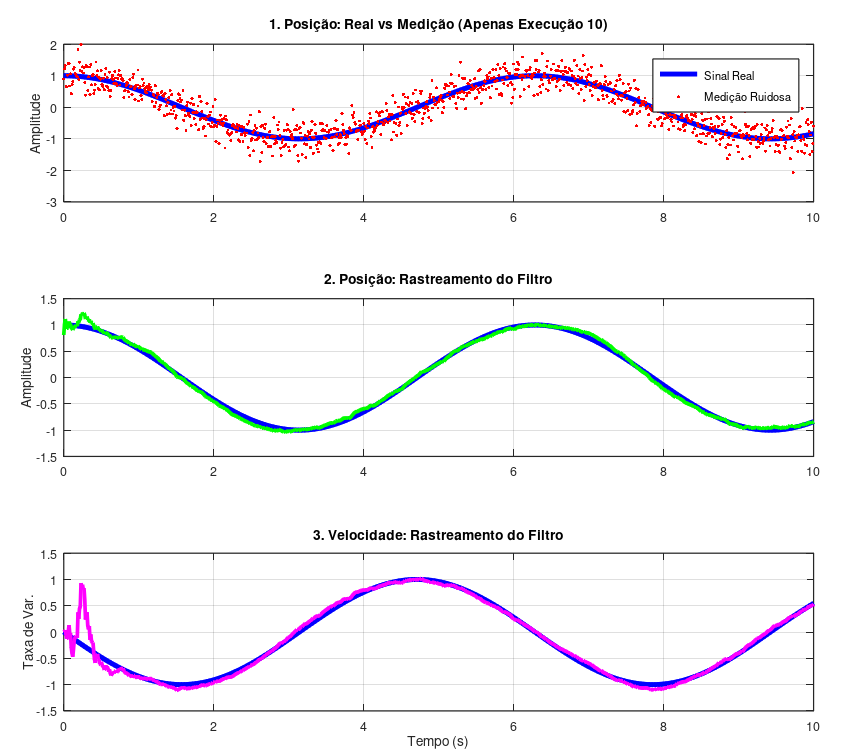
\includegraphics[width=\textwidth]{Figuras/modelo1/M1T1 - Graf.png}
        \label{fig:M1T1G}
    \end{minipage}
    \hfill
    \begin{minipage}{0.40\textwidth}
        \centering
        \caption{Erro de estimação (Teste 1).}

        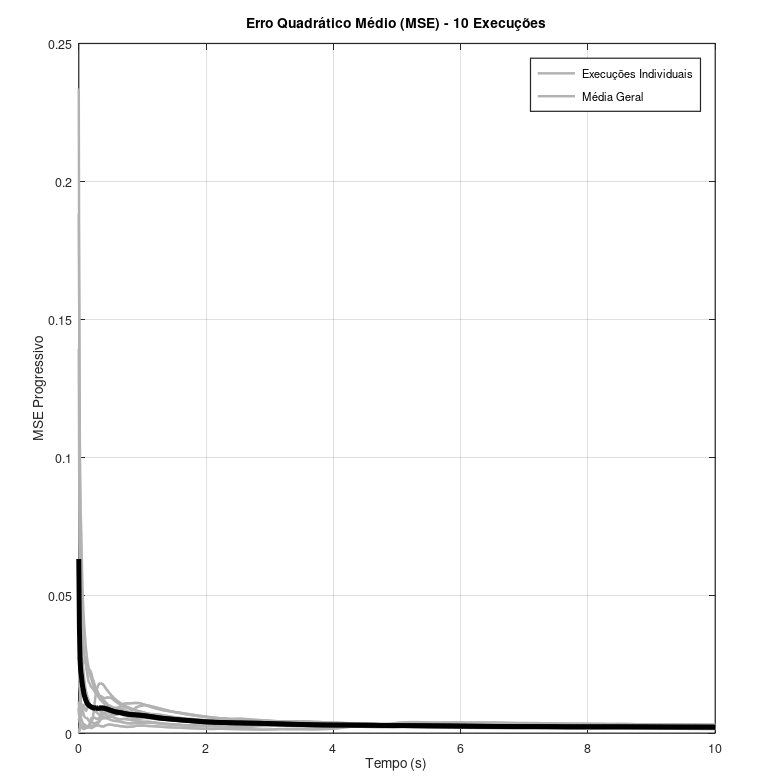
\includegraphics[width=\textwidth]{Figuras/modelo1/M1T1-Erro.png}
        \label{fig:M1T1E}
    \end{minipage}
    \caption*{\footnotesize \textbf{Fonte:} Elaborado pelo Autor (2026).}
\end{figure}

\begin{figure}[H]
    \centering
    \begin{minipage}{0.48\textwidth}
        \centering
        \caption{Rastreio nominal (Teste 2).}
        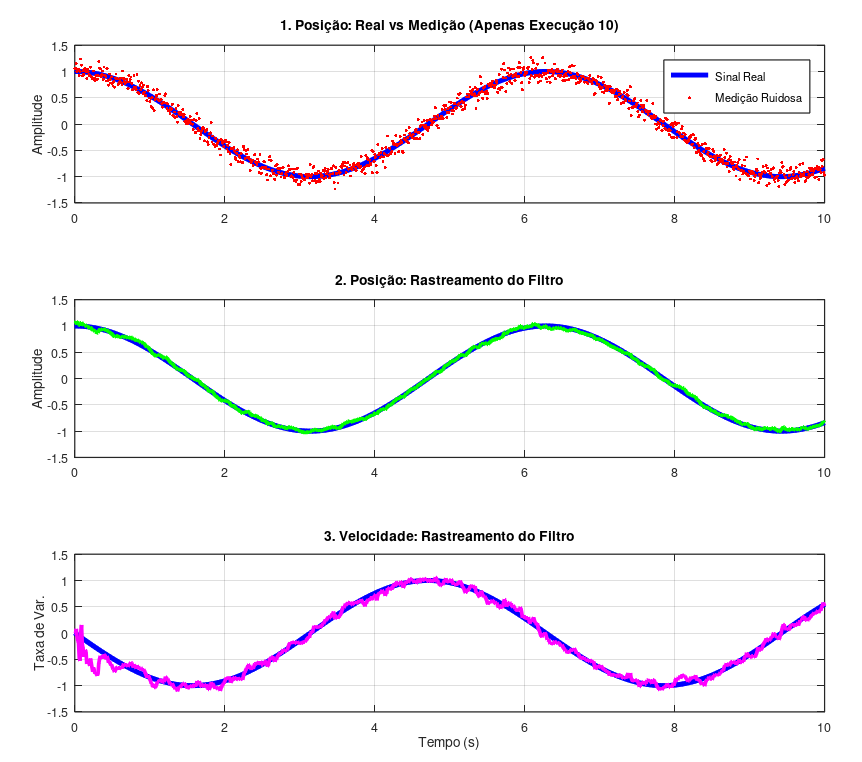
\includegraphics[width=\textwidth]{Figuras/modelo1/M1T2-G2.png}
        \label{fig:M1T2G}
    \end{minipage}
    \hfill
    \begin{minipage}{0.40\textwidth}
        \centering
        \caption{Erro de estimação (Teste 2).}
        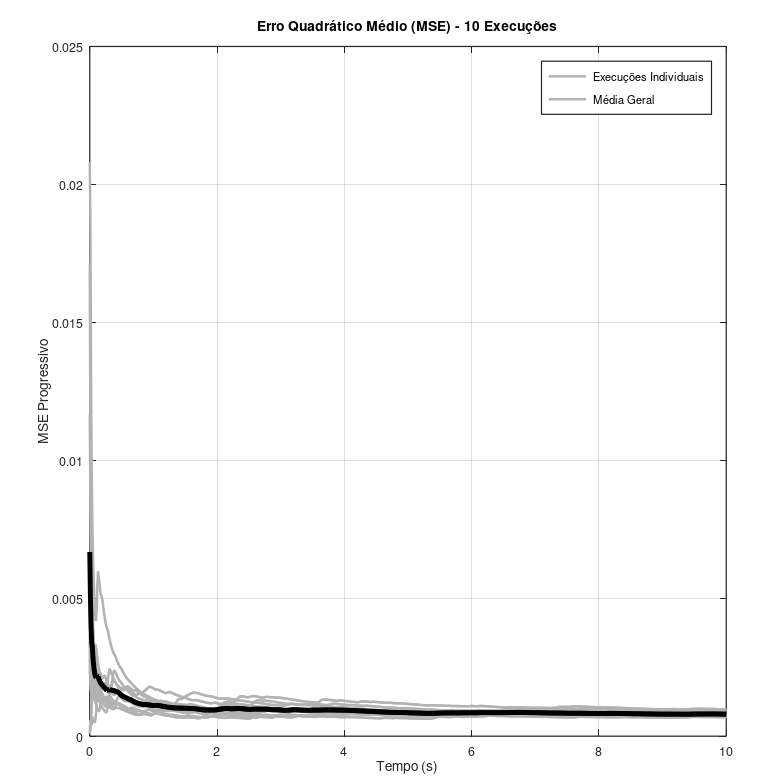
\includegraphics[width=\textwidth]{Figuras/modelo1/M1T2-E2.png}
        \label{fig:M1T2E}
    \end{minipage}
    \caption*{\footnotesize \textbf{Fonte:} Elaborado pelo Autor (2026).}
\end{figure}

\subsubsection{Teste 3: Estresse de Ruído e Incerteza Inicial}

No Teste 3, as variâncias do processo e da medição foram elevadas significativamente, acompanhadas de um erro na estimativa inicial. Este cenário avalia a robustez tempo de resposta e a estabilidade do filtro sob severa incerteza estocástica. Observou-se que devido aos ruídos com desvios superiores aos demais testes, o modelo 1 acabou tendo um filtro mais ruidoso, confome a Figura \ref{fig:M1T3G}. Como esperado, o filtro minimizou o erro rapidamente, conforme a Figura \ref{fig:M1T3E}.

\begin{figure}[H]
    \centering
    \begin{minipage}{0.48\textwidth}
        \centering
        \caption{Rastreio sob estresse (Teste 3).}
        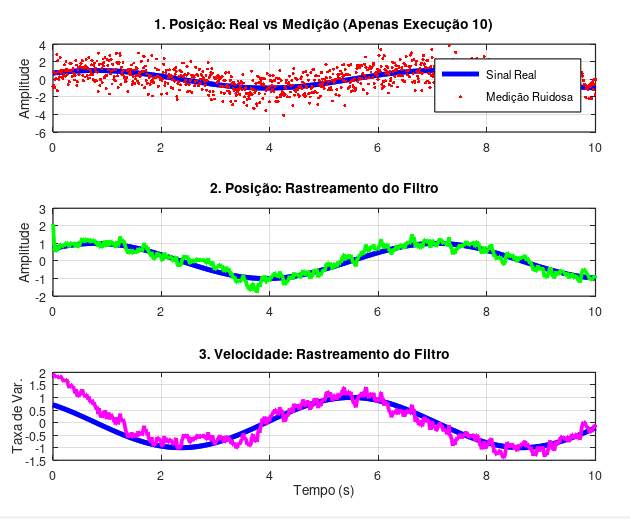
\includegraphics[width=\textwidth]{Figuras/modelo1/M1T3-GE.png}
        \label{fig:M1T3G}
    \end{minipage}
    \hfill
    \begin{minipage}{0.48\textwidth}
        \centering
        \caption{Convergência do erro (Teste 3).}
        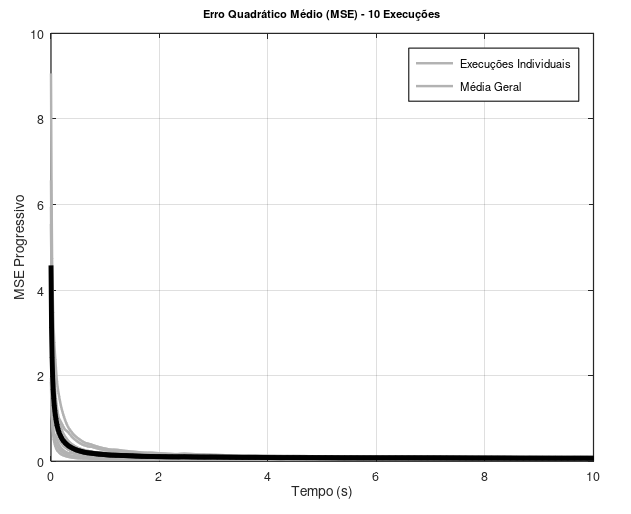
\includegraphics[width=\textwidth]{Figuras/modelo1/M1T3-ERR.png}
        \label{fig:M1T3E}
    \end{minipage}
    \caption*{\footnotesize \textbf{Fonte:} Elaborado pelo Autor (2026).}
\end{figure}

\subsubsection{Teste 4: Impacto da Não Discretização da Covariância $\mathbf{Q}$}

O Teste 4 analisa a importância da discretização correta da matriz de covariância do ruído de processo. Comparou-se o filtro projetado com a matriz contínua $\mathbf{Q} = \text{diag}(0,01; 0,1)$ contra a versão devidamente discretizada $\mathbf{Q}_k$. 

Como evidenciado nas Figuras \ref{fig:M1TFG1} a \ref{fig:M1TFE2}, a negligência quanto aos efeitos de discretização resulta em uma subestimação da incerteza do modelo, levando a um sinal de saída excessivamente ruidoso e a um aumento no erro residual, uma vez que o filtro falha em ponderar adequadamente a acumulação do ruído ao longo do intervalo $T_s$.

\begin{figure}[H]
    \centering
    \begin{minipage}{0.48\textwidth}
        \centering
        \caption{Rastreio com $\mathbf{Q}$ não discretizada.}
        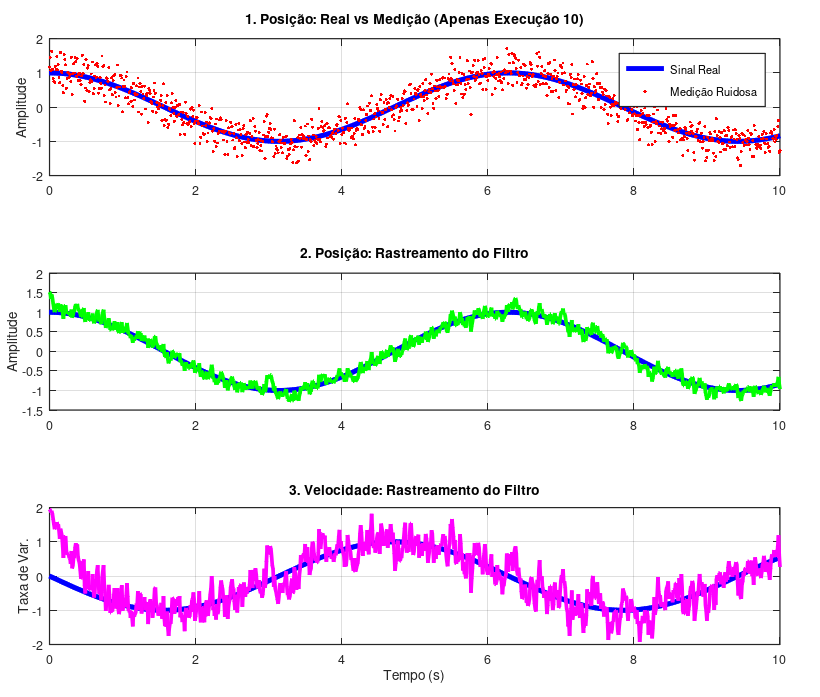
\includegraphics[width=\textwidth]{Figuras/modelo1/M1TF-GF1.png}
        \label{fig:M1TFG1}
    \end{minipage}
    \hfill
    \begin{minipage}{0.48\textwidth}
        \centering
        \caption{Rastreio com $\mathbf{Q}_k$ discreta.}
        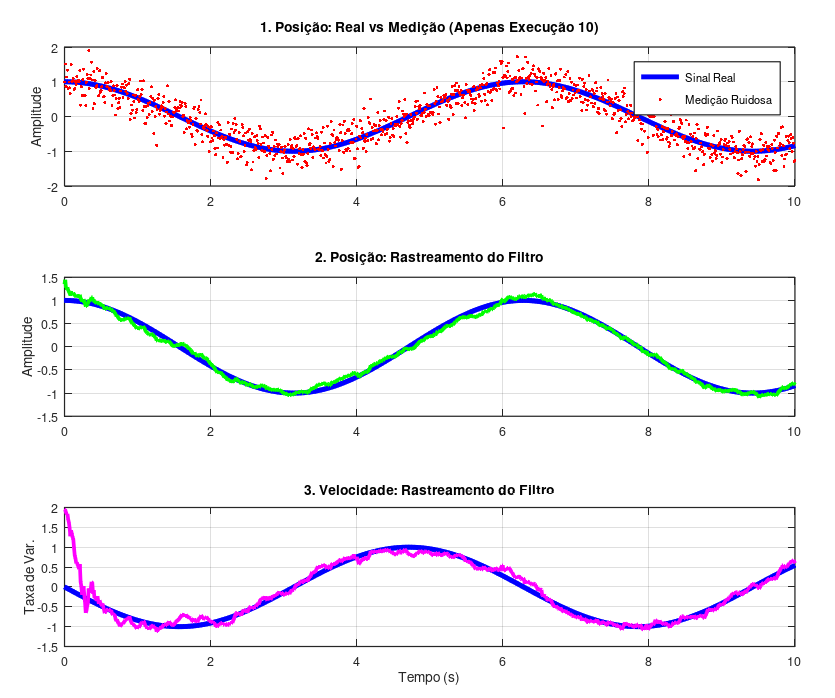
\includegraphics[width=\textwidth]{Figuras/modelo1/M1TF-GF2.png}
        \label{fig:M1TFG2}
    \end{minipage}
\end{figure}

\begin{figure}[H]
    \centering
    \begin{minipage}{0.48\textwidth}
        \centering
        \caption{Erro residual ($\mathbf{Q}$).}
        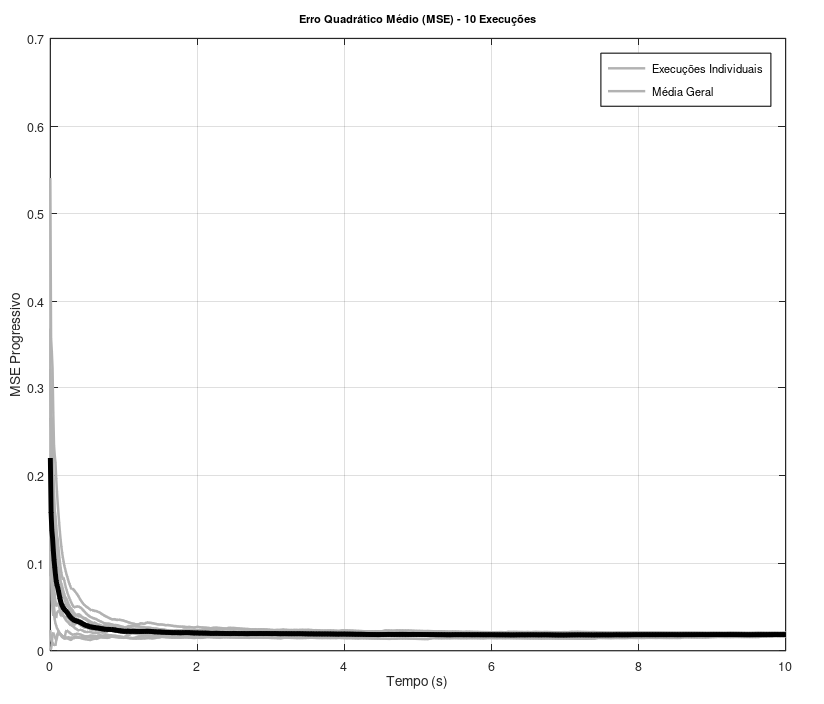
\includegraphics[width=\textwidth]{Figuras/modelo1/M1TF-EF1.png}
        \label{fig:M1TFE1}
    \end{minipage}
    \hfill
    \begin{minipage}{0.48\textwidth}
        \centering
        \caption{Erro residual ($\mathbf{Q}_k$).}
        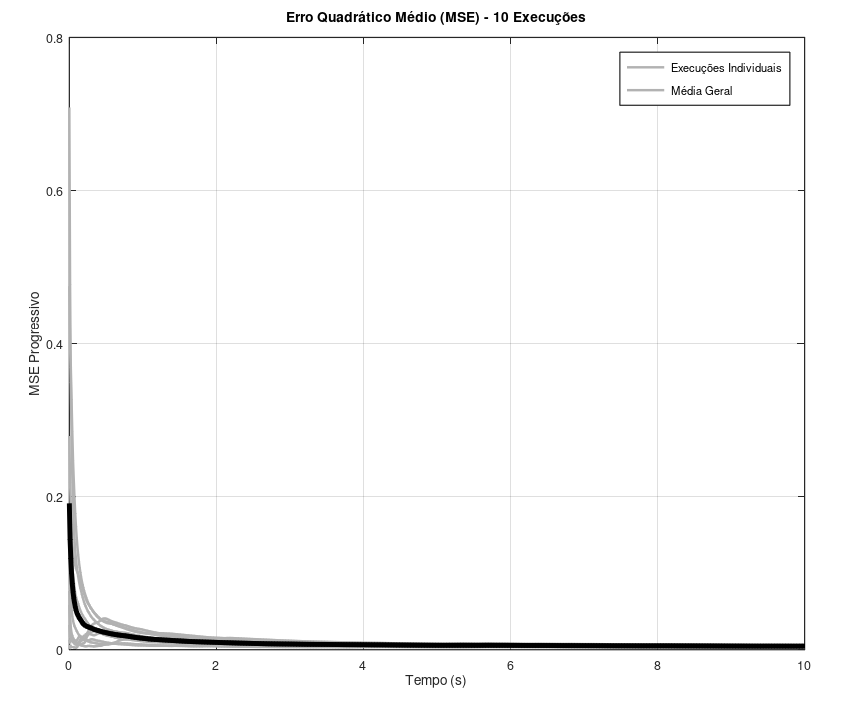
\includegraphics[width=\textwidth]{Figuras/modelo1/M1TF-EF2.png}
        \label{fig:M1TFE2}
    \end{minipage}
    \caption*{\footnotesize \textbf{Fonte:} Elaborado pelo Autor (2026).}
\end{figure}

\subsubsection{Conclusão da Parcial do Modelo 1}

Os resultados demonstram que o Modelo 1 atua satisfatoriamente como referência linear. Enquanto a convergência é mantida sob incertezas iniciais e ruído elevado, o Teste 4 destaca que a precisão do filtro é sensível à correta formulação matemática das matrizes discretas, sendo a discretização de $\mathbf{Q}$ um passo indispensável para a otimização do rastreio.

\subsection{Análise do Modelo 2: Abordagem de Três Estados ($\phi, \omega, A$)}
\label{subsec:resultados_mod2}

Relativo ao modelo 2 (modelado na Subseção \ref{subsubsec:modelo2}), a formulação visa a estimação simultânea da fase ($\phi$), frequência angular ($\omega$) e amplitude ($A$). Diferente do modelo linear anterior, esta abordagem lida com uma estrutura não linear, o que exige maior precisão na inicialização do filtro. Embora o modelo apresente desempenho satisfatório em condições ideais, observou-se uma sensibilidade crítica aos parâmetros iniciais, podendo resultar em falhas de observabilidade.

Foram realizadas 10 repetições independentes (Monte Carlo) para cada configuração de teste. As figuras apresentadas nas subseções ilustram a décima execução como exemplo; nos gráficos de Monte Carlo a curva preta representa a média das 10 execuções e as curvas em tons de cinza representam as execuções individuais.

Os parâmetros configurados para os três ensaios do Modelo 2 estão detalhados na Tabela \ref{tab:parametros_m2}.

\begin{table}[H]
\centering
\caption{Parâmetros de simulação para os testes do Modelo 2.}
\label{tab:parametros_m2}
\begin{tabular}{l|c|c|c}
\hline
	extbf{Parâmetro} & \textbf{Teste 1} & \textbf{Teste 2} & \textbf{Teste 3} \\ \hline
$T_s$ (Amostragem) & \multicolumn{3}{c}{0,01 segundos} \\
Tempo Total & \multicolumn{3}{c}{10 segundos} \\ 
Monte Carlo & \multicolumn{3}{c}{10 repetições} \\ 
Amplitude (A) & \multicolumn{3}{c}{1,5} \\ 
$\omega$ & \multicolumn{3}{c}{1,2 rad/s} \\ 
$\phi_0$ & \multicolumn{3}{c}{0 rad} \\ \hline
$\sigma^2_{w1}, \sigma^2_{w2}, \sigma^2_{w3}$ & 0,001; 0,001; 0,01 & 0,001; 0,001; 0,01 & 0,001; 0,001; 0,01 \\ 
$R$ (Medição) & 0,05 & 0,1 & 0,1 \\ 
$\hat{\mathbf{x}}_0$ (Inicial) & $[0; 1; 1]^T$ & $[0; 1; -1]^T$ & $[0; -1; -1]^T$ \\ \hline
\end{tabular}
\end{table}

\subsubsection{Teste 1: Cenário Nominal e Convergência Ideal}

No \textbf{Teste 1}, o filtro foi inicializado sob condições nominais, utilizando estimativas iniciais próximas aos parâmetros reais e um baixo ruído de processo. O objetivo deste cenário é validar a estabilidade e a capacidade de rastreamento do algoritmo em regime estacionário. Conforme ilustrado na Figura \ref{fig:M2T1G}, as estimativas de fase e amplitude apresentam convergência rápida, mantendo um erro residual estatisticamente coerente com a variância do ruído de medição ($R = 0,05$).
\begin{figure}[H]
    \centering
    \caption{Modelo 2: Estimativas (Teste 1).}
    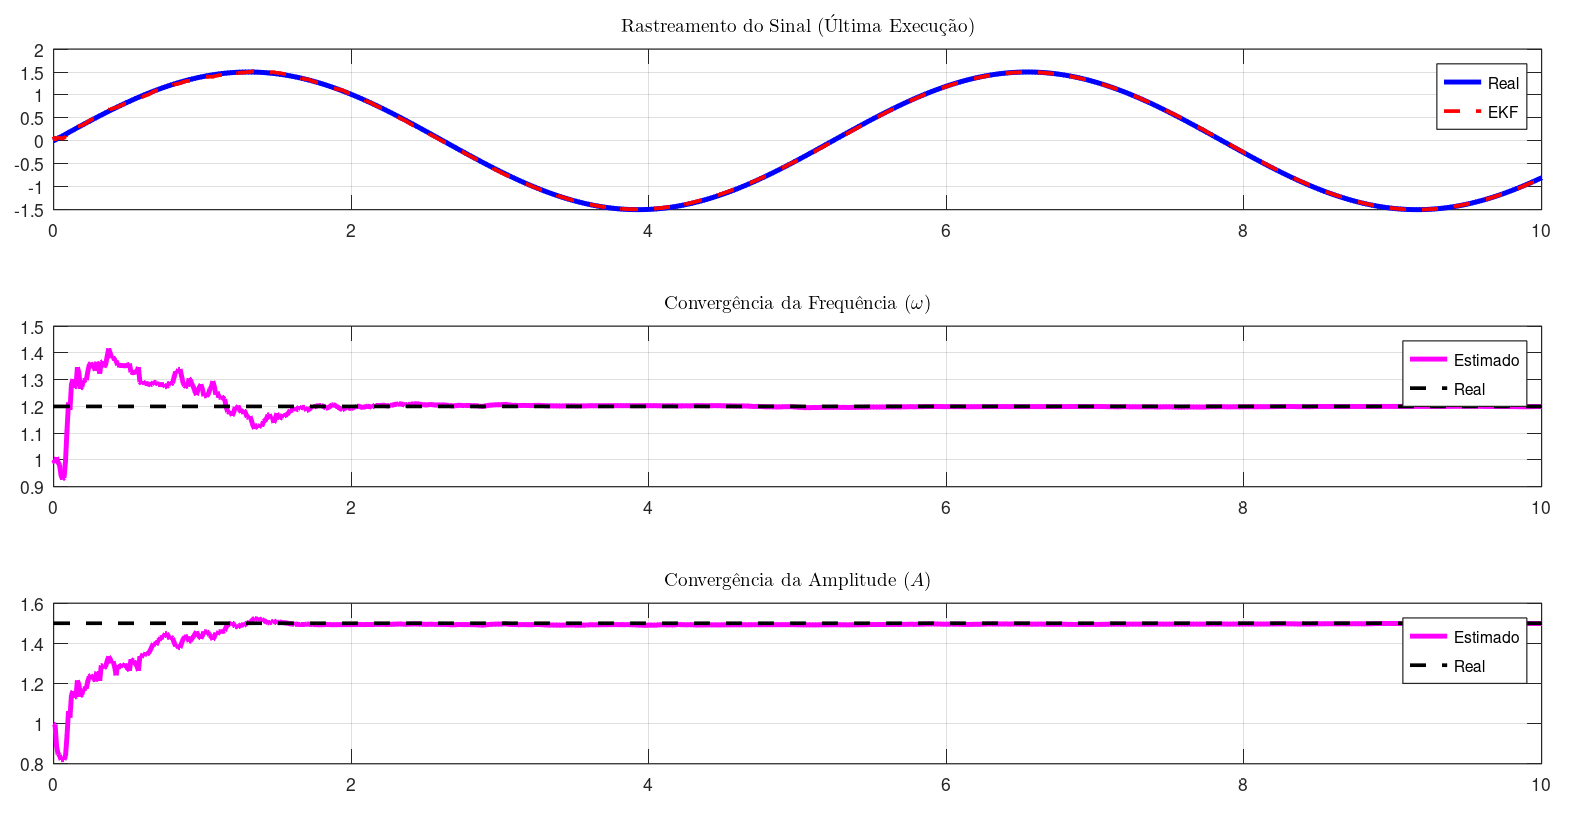
\includegraphics[width=12cm]{Figuras/modelo2/M2T1-GE.png}
    \label{fig:M2T1G}
    \caption*{\footnotesize \textbf{Fonte:} Elaborado pelo Autor (2026).}
\end{figure}


Quanto ao desempenho estocástico, a evolução do Erro Quadrático Médio (MSE) confirma a eficácia do estimador na filtragem do ruído. A redução progressiva observada na Figura \ref{fig:M2T1CONV_CO}(a) indica que as incertezas dos estados internos decaem para níveis satisfatórios de precisão após o transiente inicial. Paralelamente, o erro de saída (Figura \ref{fig:M2T1CONV_CO}b) é minimizado conforme o filtro converge, atingindo o critério de otimalidade esperado para a formulação de Kalman neste cenário de erro de modelo nulo.

\begin{figure}[H]
    \centering
    \caption{Modelo 2: Convergências do erro (Teste 1).}
    \begin{minipage}{0.48\textwidth}
        \centering
        \caption*{\footnotesize \textbf{(a) MSE dos Estados ($\phi, \omega, A$).}}
        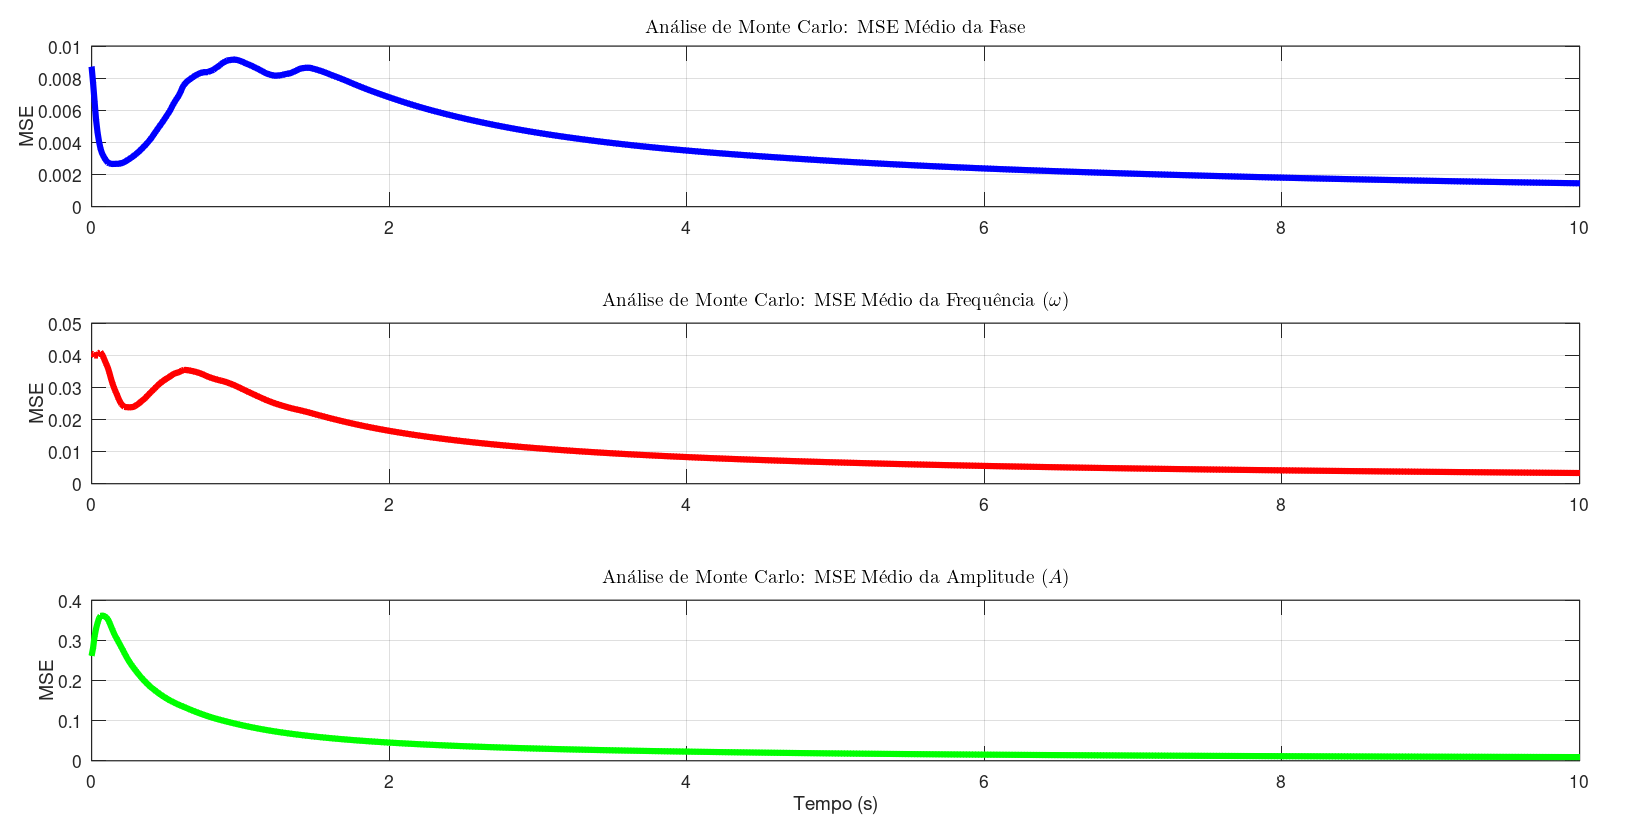
\includegraphics[width=\textwidth]{Figuras/modelo2/M2T1-GER.png}
    \end{minipage}\hfill
    \begin{minipage}{0.48\textwidth}
        \centering
        \caption*{\footnotesize \textbf{(b) MSE da Saída (Monte Carlo)}}
        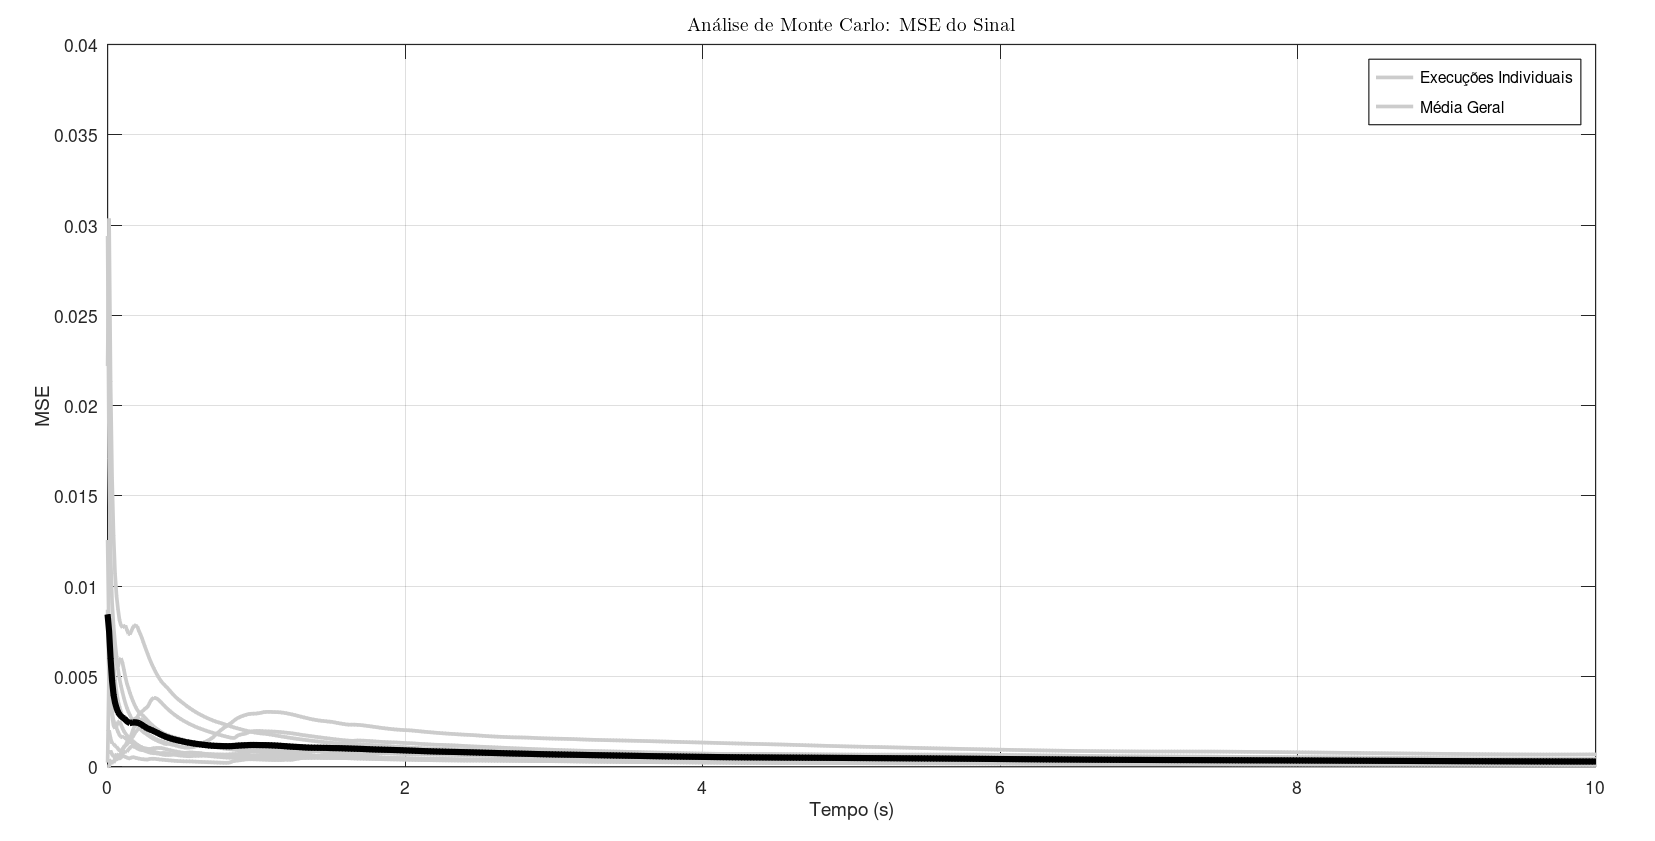
\includegraphics[width=\textwidth]{Figuras/modelo2/M2T1-GERR.png}
    \end{minipage}
    \caption*{\footnotesize \textbf{Fonte:} Elaborado pelo Autor (2026).}
    \label{fig:M2T1CONV_CO}
\end{figure}

\subsubsection{Teste 2: Inversão de Frequência 1}
\label{subsubsec:res_m2_t2}

O \textbf{Teste 2} explora a robustez do filtro diante de erros grosseiros na inicialização da frequência ($\omega$). Devido à identidade trigonométrica $-A \sin(-\omega t) = A \sin(\omega t)$, o processo de observação apresenta uma ambiguidade inerente. Caso a estimativa inicial $\hat{\omega}_0$ possua sinal oposto ao valor real, o filtro tende a convergir para um \textit{mínimo local} de erro.

Neste cenário, para compensar a inversão da dinâmica temporal, o algoritmo estima uma amplitude negativa ou introduz um deslocamento de fase de $180^\circ$ (equivalente a $\pi$ radianos). Como observado na Figura \ref{fig:M2T2G}, o filtro consegue reconstruir o sinal de saída com precisão, mas falha na identificação dos parâmetros físicos internos. Estatisticamente, isso resulta em um Erro Quadrático Médio de saída reduzido (Figura \ref{fig:M2T2CONV_CO}b), contrastando com um MSE de estados elevado (Figura \ref{fig:M2T2CONV_CO}a), o que caracteriza uma falha de observabilidade parcial sob condições de inicialização adversas.

\begin{figure}[H]
    \centering
    \caption{Modelo 2: Estimativas de estado e sinal (Teste 2).}
    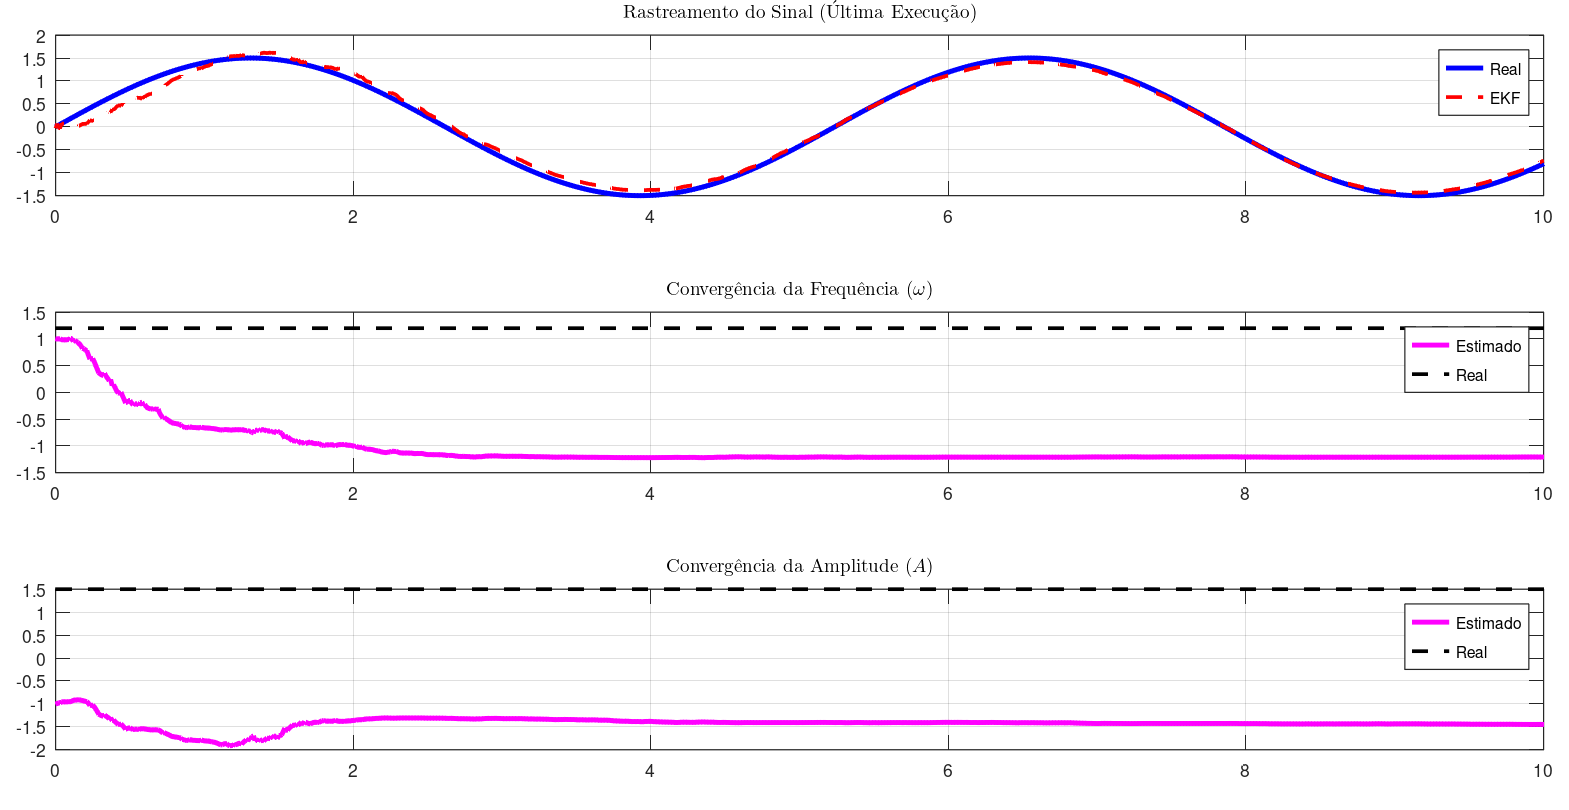
\includegraphics[width=12cm]{Figuras/modelo2/M2T2-GE.png}
    \label{fig:M2T2G}
    \caption*{\footnotesize \textbf{Fonte:} Elaborado pelo Autor (2026).}
\end{figure}

\begin{figure}[H]
    \centering
    \caption{Modelo 2: Análise de convergência e erro (Teste 2).}
    \begin{minipage}{0.48\textwidth}
        \centering
        \caption*{\footnotesize \textbf{(a) MSE dos Estados ($\phi, \omega, A$).}}
        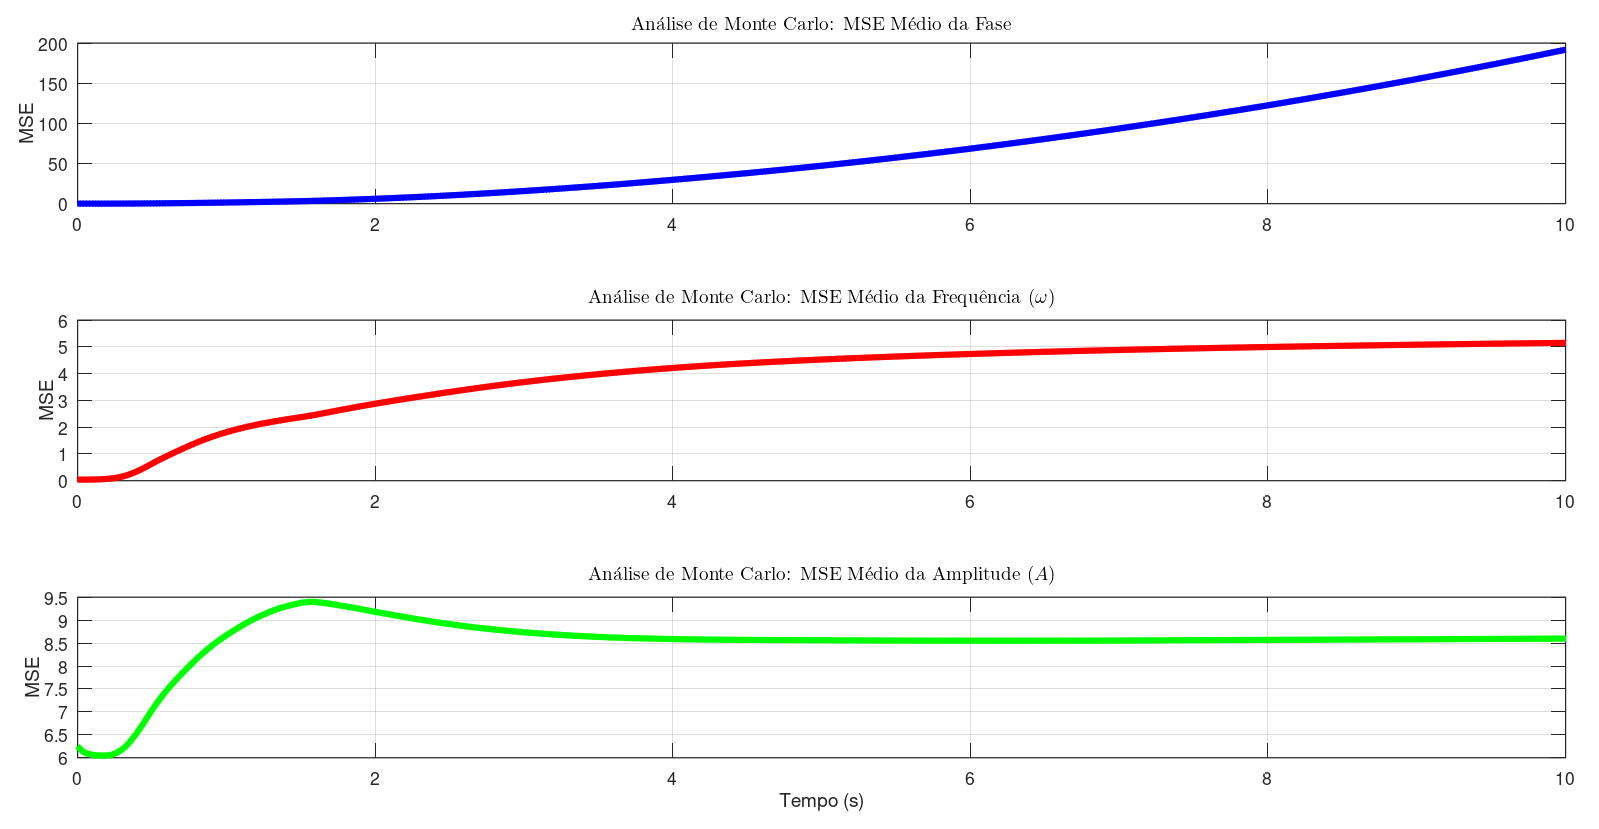
\includegraphics[width=\textwidth]{Figuras/modelo2/M2T2-GER.png}
    \end{minipage}\hfill
    \begin{minipage}{0.48\textwidth}
        \centering
        \caption*{\footnotesize \textbf{(b) MSE da Saída (Monte Carlo)}}
        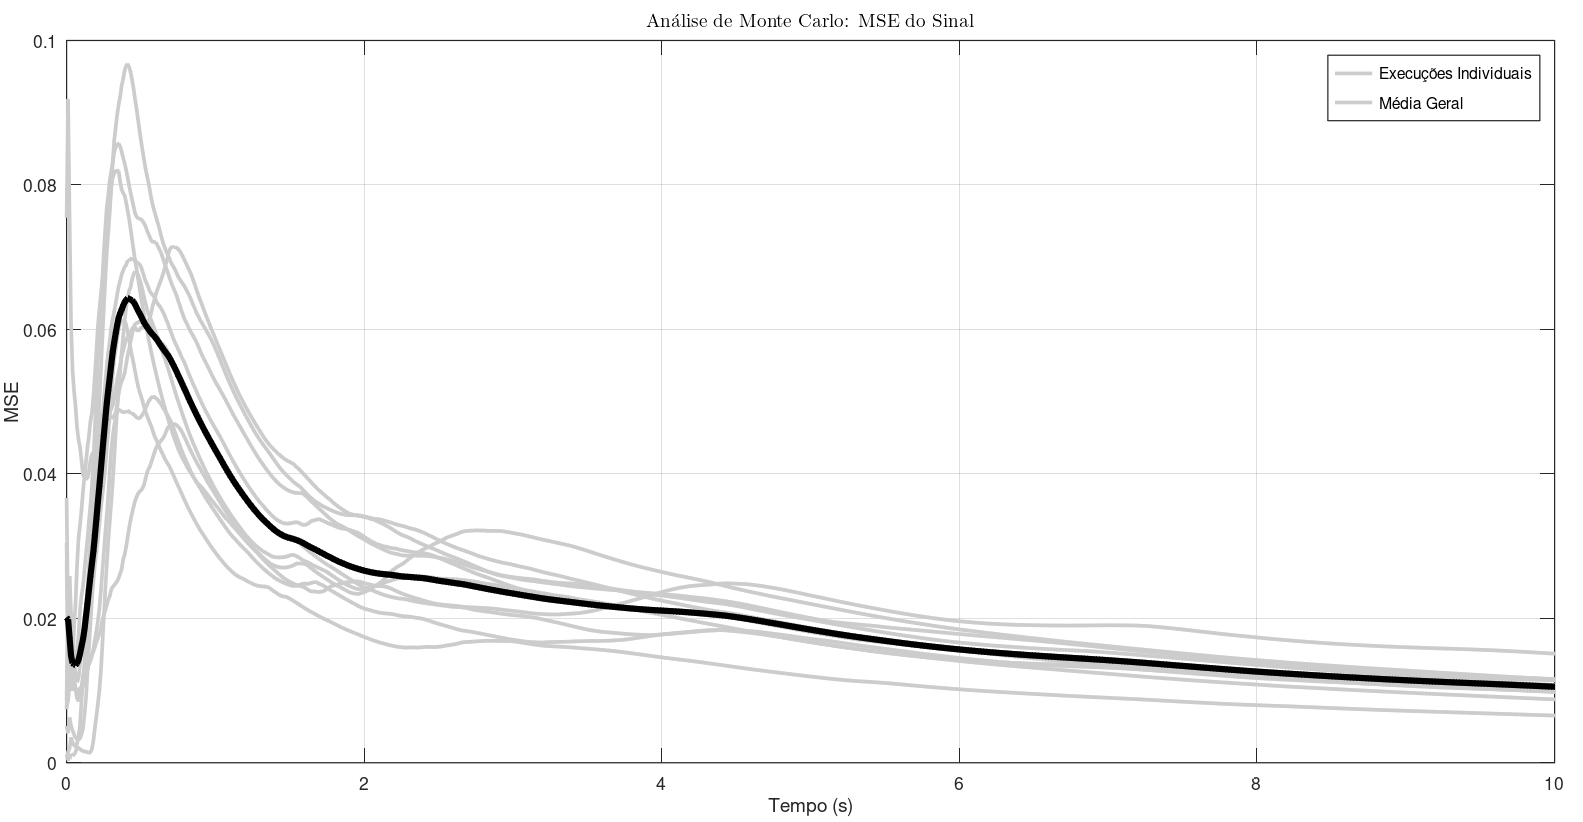
\includegraphics[width=\textwidth]{Figuras/modelo2/M2T2-GERR.png}
    \end{minipage}
    \caption*{\footnotesize \textbf{Fonte:} Elaborado pelo Autor (2026).}
    \label{fig:M2T2CONV_CO}
\end{figure}

\subsubsection{Teste 3: Inversão de Frequência 2}
\label{subsubsec:res_m2_t3}

O \textbf{Teste 3} avalia o comportamento do filtro em cenários de forte incompatibilidade entre o modelo interno e a dinâmica real. As estimativas transientes, apresentadas na Figura \ref{fig:M2T3G}, revelam a dificuldade inicial do EKF em sincronizar com a frequência portadora quando o erro de inicialização ultrapassa os limites de linearidade da Jacobiana.

A análise do Erro Quadrático Médio na Figura \ref{fig:M2T3CONV_CO} demonstra que, embora o filtro busque a minimização do erro de saída para garantir o rastreamento do sinal, o custo computacional e o tempo de convergência dos estados internos são significativamente superiores aos observados no Teste 1. Este comportamento reforça a sensibilidade do Modelo 2 às condições de contorno, evidenciando a necessidade de modelos mais adaptativos, como os que serão discutidos nas seções subsequentes.

\begin{figure}[H]
    \centering
    \caption{Modelo 2: Estimativas de estado e sinal (Teste 3).}
    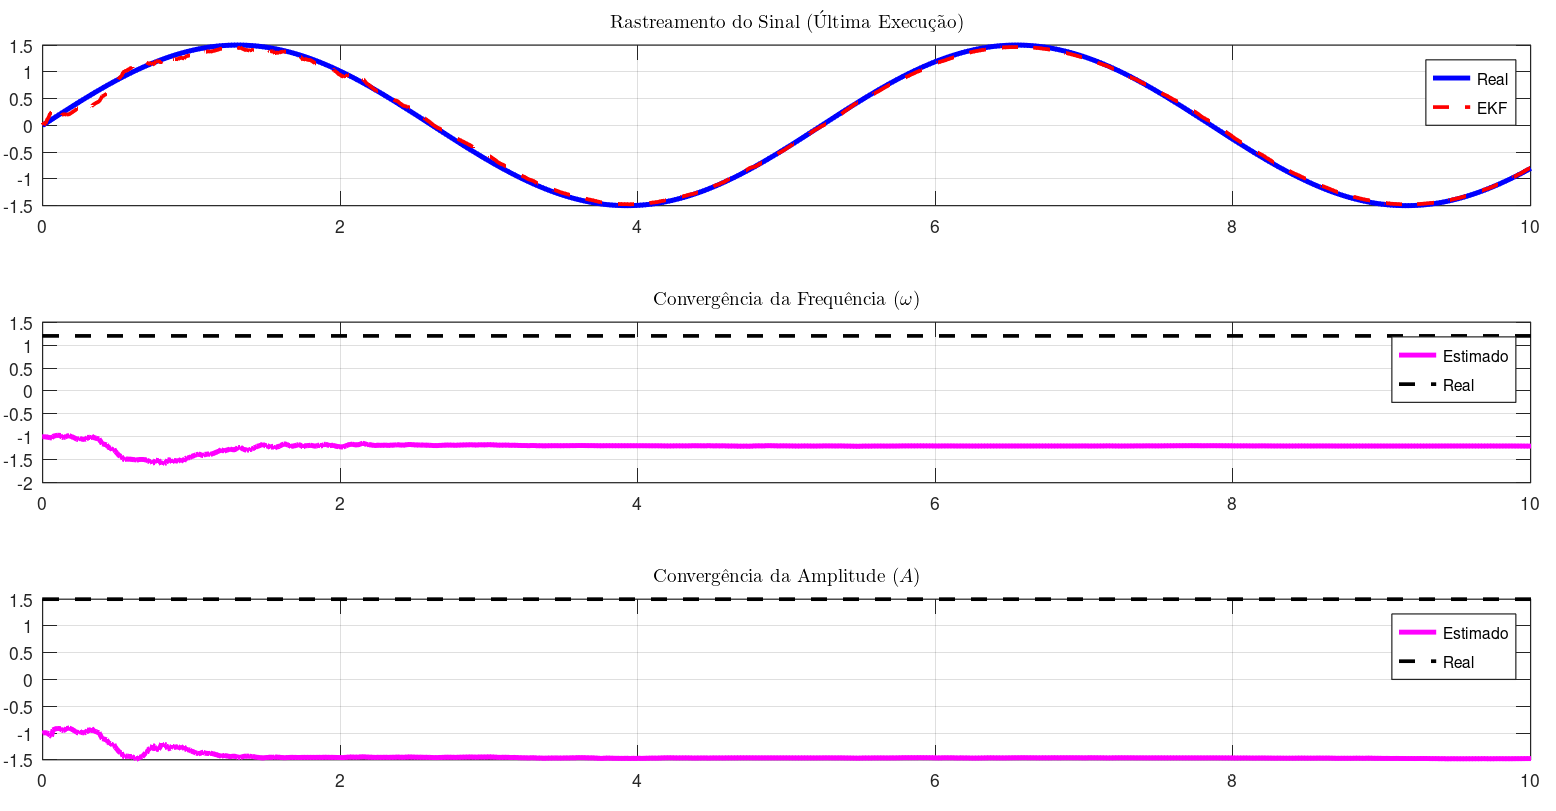
\includegraphics[width=12cm]{Figuras/modelo2/M2T3-GE.png}
    \label{fig:M2T3G}
    \caption*{\footnotesize \textbf{Fonte:} Elaborado pelo Autor (2026).}
\end{figure}

\begin{figure}[H]
    \centering
    \caption{Modelo 2: Análise de convergência e erro (Teste 3).}
    \begin{minipage}{0.48\textwidth}
        \centering
        \caption*{\footnotesize \textbf{(a) MSE dos Estados ($\phi, \omega, A$).}}
        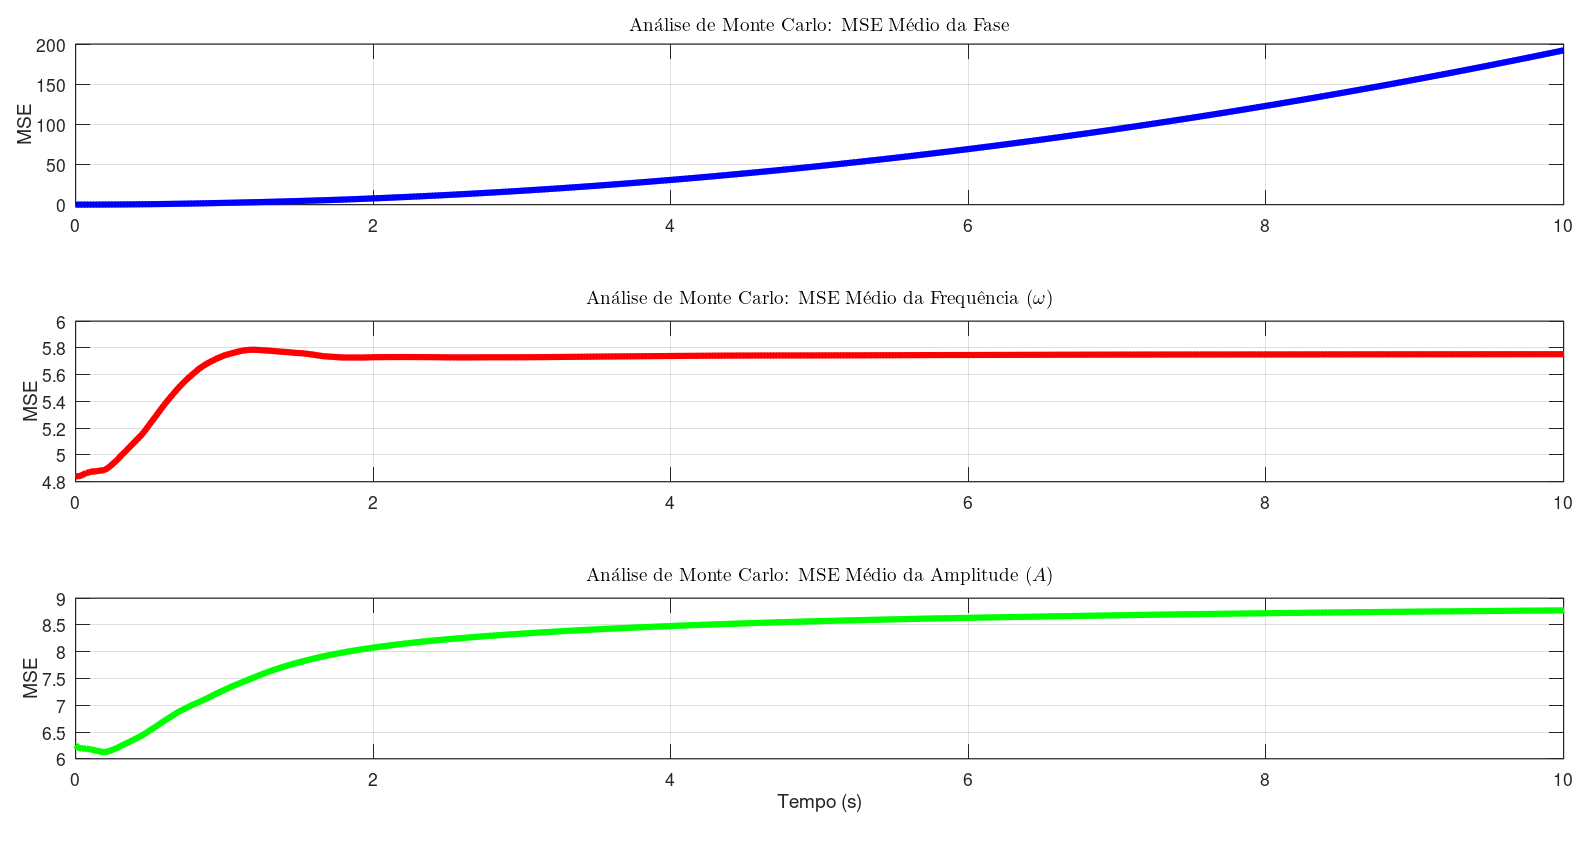
\includegraphics[width=\textwidth]{Figuras/modelo2/M2T3-GER.png}
    \end{minipage}\hfill
    \begin{minipage}{0.48\textwidth}
        \centering
        \caption*{\footnotesize \textbf{(b) MSE da Saída (Monte Carlo).}}
        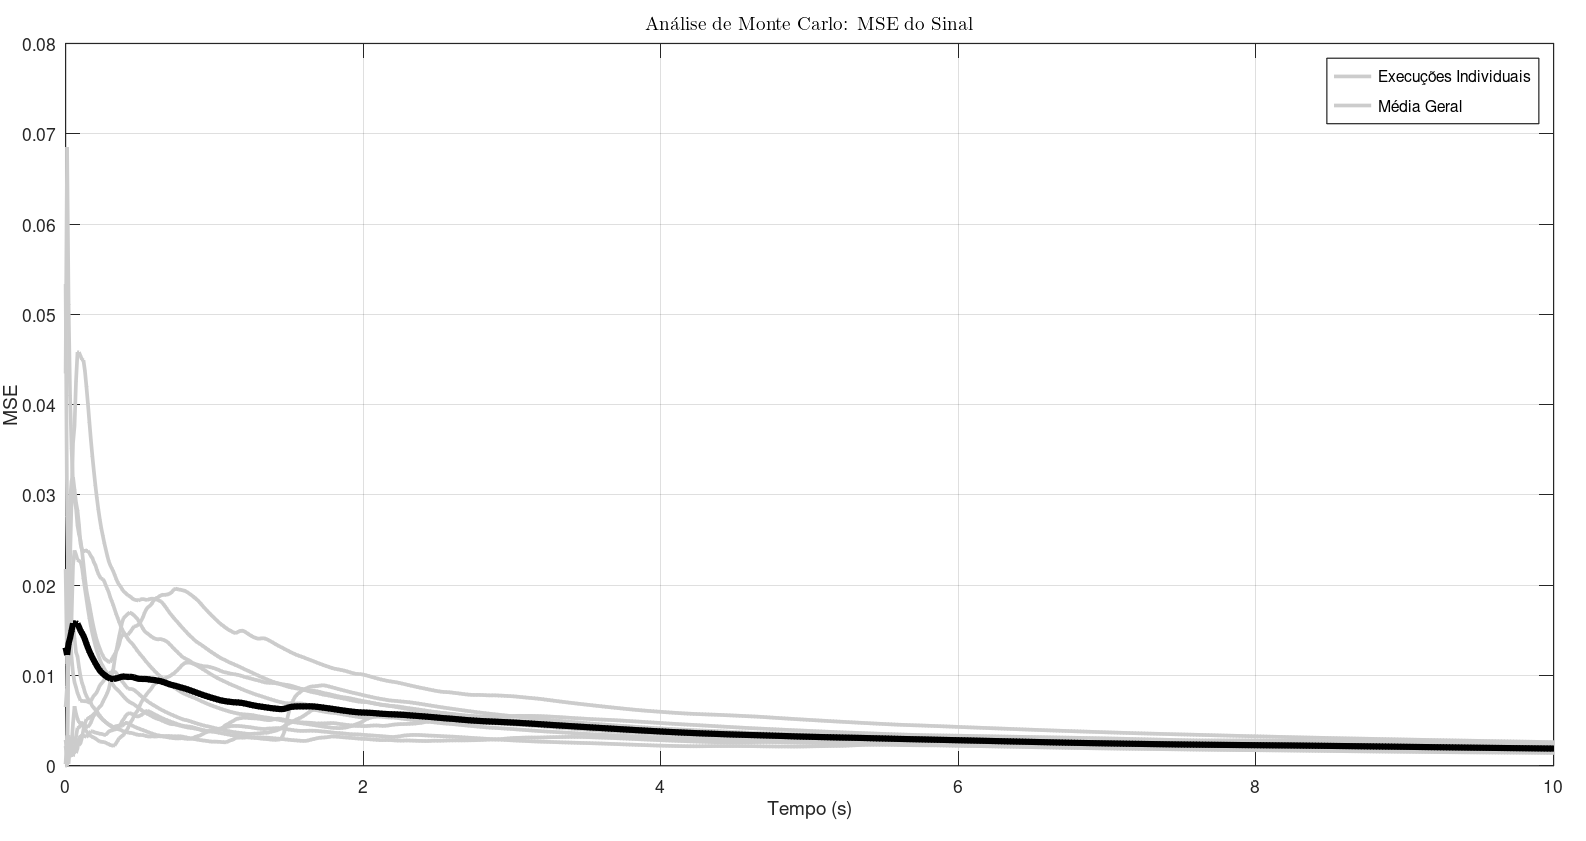
\includegraphics[width=\textwidth]{Figuras/modelo2/M2T3-GERR.png}
    \end{minipage}
    \caption*{\footnotesize \textbf{Fonte:} Elaborado pelo Autor (2026).}
    \label{fig:M2T3CONV_CO}
\end{figure}

\subsubsection{Conclusão Parcial do Modelo 2}

Os resultados obtidos nas simulações do Modelo 2  corroboram as conclusões apresentadas por \citeonline{zarchan2015}, evidenciando que o desempenho deste EKF é estritamente dependente da acurácia da inicialização. Verificou-se que, em regimes onde a frequência real e a estimativa inicial compartilham o mesmo sinal algébrico ($\mathrm{sgn}(\omega_{real}) = \mathrm{sgn}(\hat{\omega}_0)$), o filtro apresenta uma convergência estável e fisicamente coerente dos estados de amplitude e fase.

Contudo, os cenários de incompatibilidade (Teste 2 e 3) revelaram a fragilidade do modelo frente às ambiguidades da função seno. Assim como reportado pelo autor, observou-se que o filtro converge para \textit{mínimos locais} não físicos quando os sinais são opostos; embora o rastreamento do sinal de saída seja mantido, a integridade dos estados internos é comprometida por inversões de sinal na amplitude ou deslocamentos espúrios de fase. 

Em suma, a experiência prática ratifica que a escolha da representação dos estados no Modelo 2 limita a observabilidade global do sistema. Os resultados semelhantes aos da literatura confirmam que, apesar de funcional para rastreamento básico, este modelo carece de robustez para aplicações onde a direção da dinâmica (\textit{frequência positiva ou negativa}) não é conhecida a priori, justificando a exploração de arquiteturas mais resilientes, como os Modelos 4 e 5.

\subsection{Análise do Modelo 3: Redução de Ordem e Estabilização ($\phi, \omega$)}
\label{subsec:resultados_mod3}

Foram realizadas 10 repetições independentes (Monte Carlo) para cada configuração de teste. As figuras apresentadas nas subseções ilustram a décima execução como exemplo; nos gráficos de Monte Carlo a curva preta representa a média das 10 execuções e as curvas em tons de cinza representam as execuções individuais.

O Modelo 3 (modelado na Subseção \ref{subsubsec:modelo3}) foi proposto para mitigar as falhas de observabilidade identificadas na abordagem anterior. Ao assumir a amplitude $A$ como uma constante conhecida e positiva, o filtro é reduzido para dois estados ($\phi, \omega$). Esta simplificação elimina a ambiguidade matemática $-A \sin(-\omega t) = A \sin(\omega t)$, uma vez que, com $A$ fixo, apenas a convergência para a frequência angular com o sinal correto minimiza o erro quadrático médio.

Os parâmetros utilizados para validar a robustez desta abordagem estão consolidados na Tabela \ref{tab:parametros_m3}. Conforme modelado na sessão \ref{subsubsec:modelo3}, adotou-se um $\sigma^2 _{w1} = 0$.

\begin{table}[H]
\centering
\caption{Parâmetros de simulação para os testes do Modelo 3.}
\label{tab:parametros_m3}
\begin{tabular}{l|c|c|c}
\hline
\textbf{Parâmetro} & \textbf{Teste 1} & \textbf{Teste 2} & \textbf{Teste 3} \\ \hline
$T_s$ (Amostragem) & \multicolumn{3}{c}{0,01 segundos} \\
Tempo Total & \multicolumn{3}{c}{10 segundos} \\ 
Monte Carlo & \multicolumn{3}{c}{10 repetições} \\ 
Amplitude (A) & \multicolumn{3}{c}{1,5} \\ \hline
$\omega$ & 1,2 rad/s & 1,2 rad/s & -1,2 rad/s  \\ \hline
$\phi_0$ & \multicolumn{3}{c}{0 rad} \\ \hline
$\sigma^2_{w1}, \sigma^2_{w2}$ & 0; 0,001 & 0; 0,001 & 0; 0,001 \\ 
$R$ (Medição) & 0,1 & 0,1 & 0,1 \\ 
$\hat{\mathbf{x}}_0$ (Inicial) & $[0; 1]^T$ & $[0; -1]^T$ & $[0; 1]^T$ \\ \hline
\end{tabular}
\end{table}

\subsubsection{Teste 1: Desempenho em Cenário Nominal}

No cenário nominal, o Modelo 3 apresenta uma convergência superior ao Modelo 2, com menor tempo de acomodação para a frequência angular. A ausência da amplitude como estado a ser estimado reduz o acoplamento não linear, resultando em um rastreio mais limpo e estável (conforme a Figura \ref{fig:M3T1G}). A diminuição dos erros quadráticos médios é observado na Figura \ref{fig:M3T1CONV_CO}.

\begin{figure}[H]
    \centering
    \caption{Modelo 3: Estimativas (Teste 1).}
    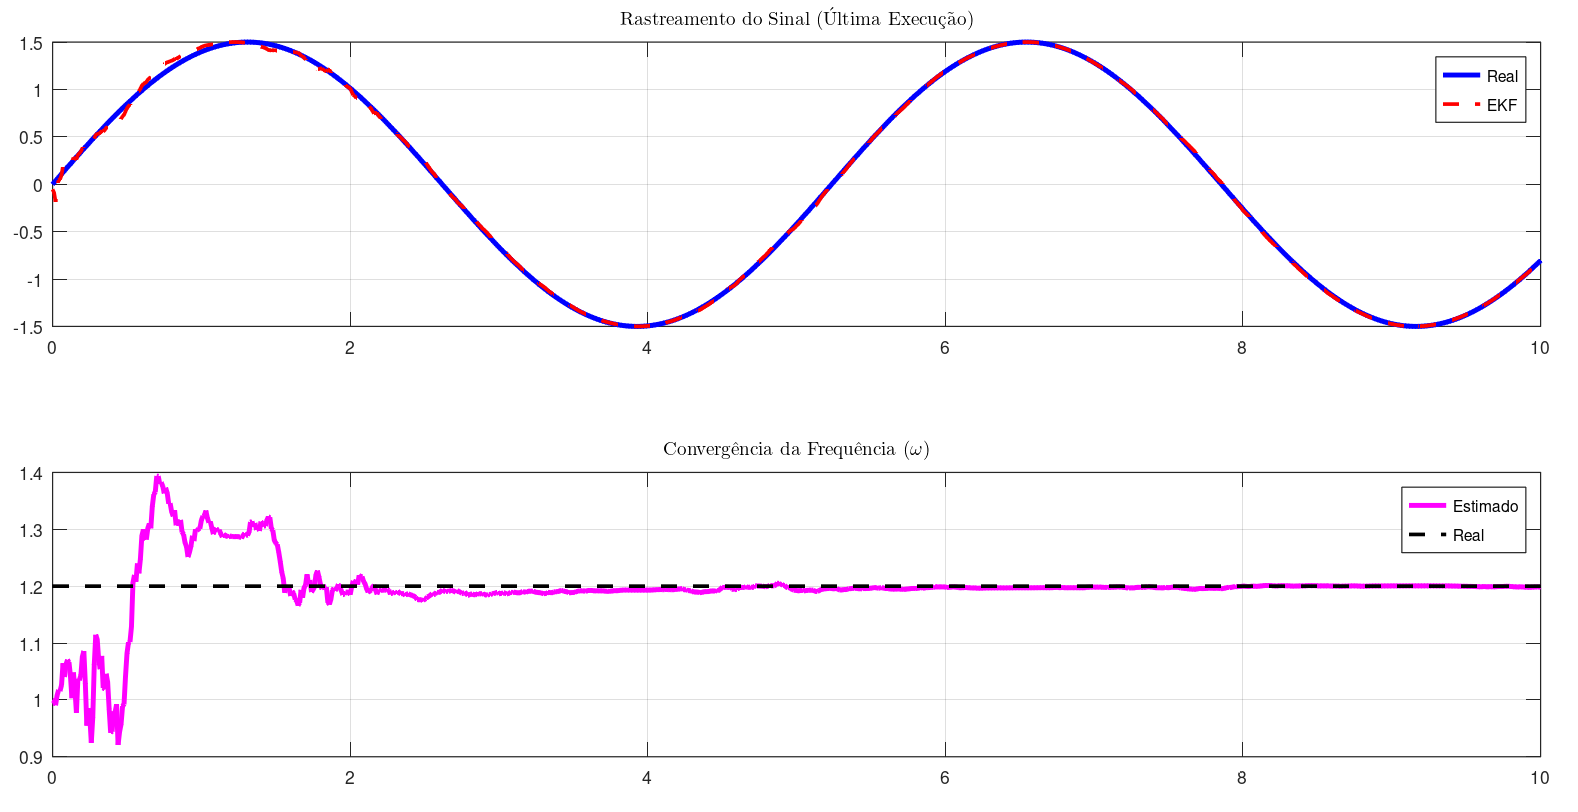
\includegraphics[width=14cm]{Figuras/modelo3/M3T1-GE.png}
    \label{fig:M3T1G}
    \caption*{\footnotesize \textbf{Fonte:} Elaborado pelo Autor (2026).}
\end{figure}

\begin{figure}[H]
    \centering
    \caption{Modelo 3: Convergências do erro (Teste 1).}
    \begin{minipage}{0.48\textwidth}
        \centering
        \caption*{\footnotesize \textbf{(a) MSE dos Estados ($\phi, \omega$)}}
        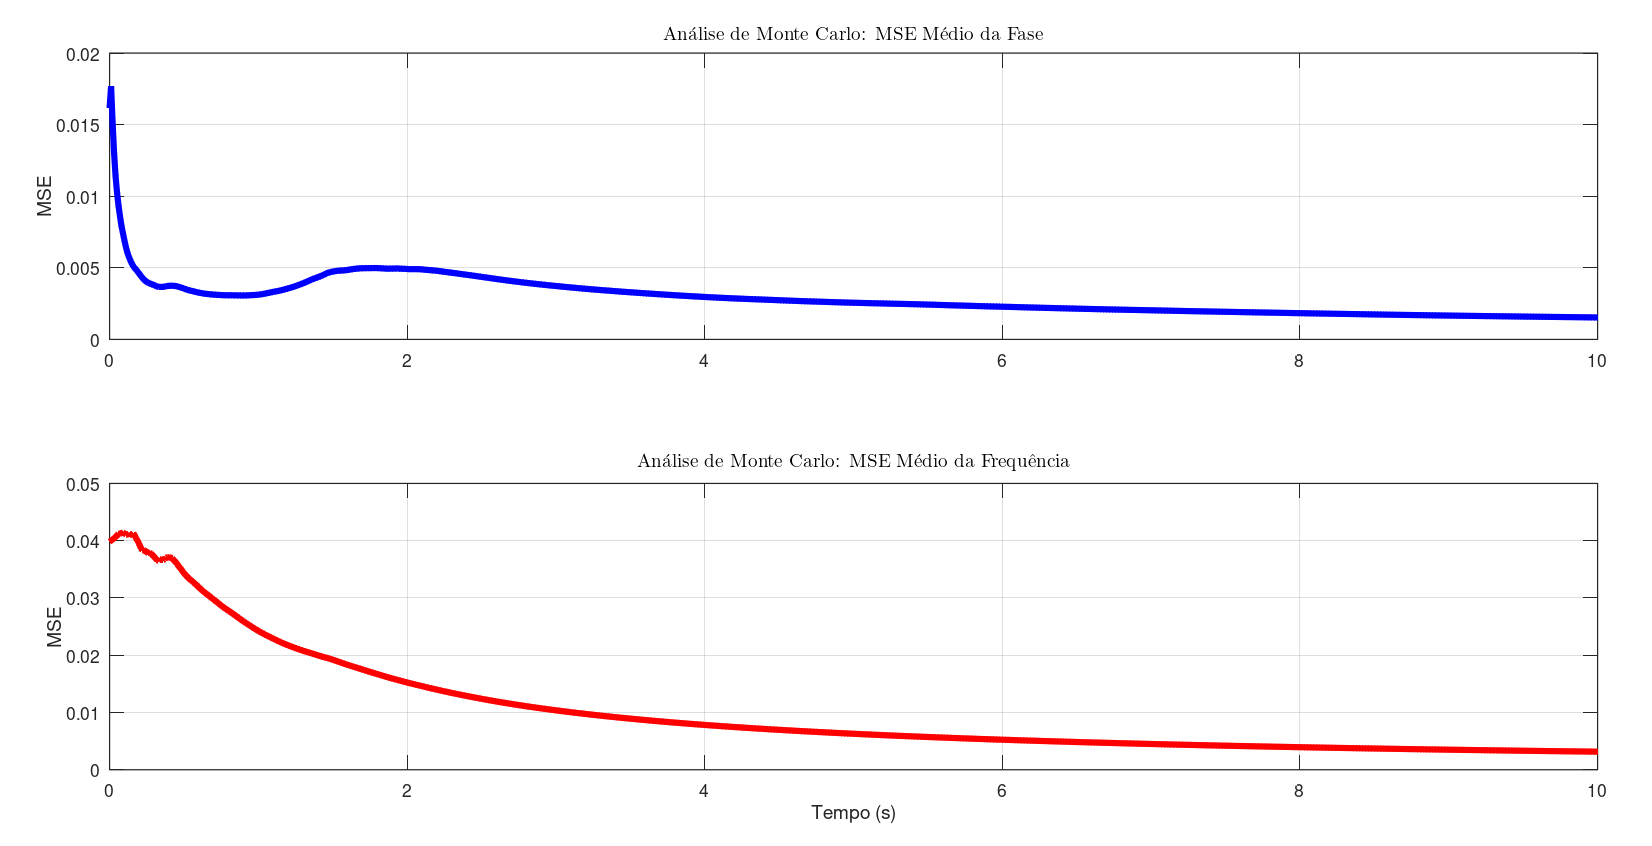
\includegraphics[width=\textwidth]{Figuras/modelo3/M3T1-GER.png}
    \end{minipage}\hfill
    \begin{minipage}{0.48\textwidth}
        \centering
        \caption*{\footnotesize \textbf{(b) MSE de Saída (Monta Carlo)}}
        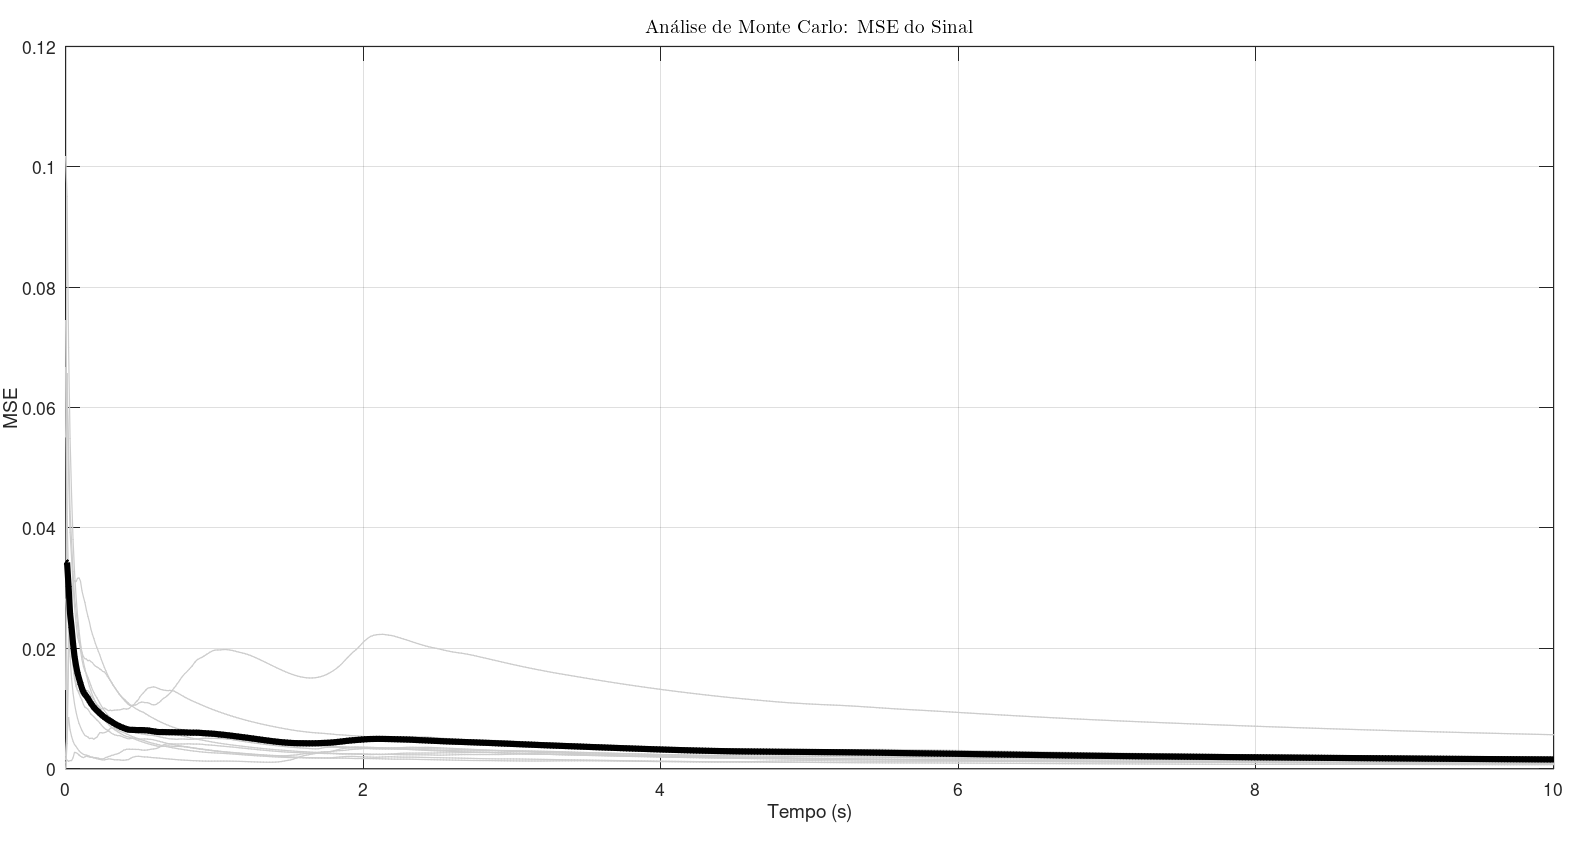
\includegraphics[width=\textwidth]{Figuras/modelo3/M3T1-GERR.png}
    \end{minipage}
    \caption*{\footnotesize \textbf{Fonte:} Elaborado pelo Autor (2026).}
    \label{fig:M3T1CONV_CO}
\end{figure}

\subsubsection{Teste 2: Robustez à Inversão de Sinais e Ambiguidade}
\label{subsubsec:m3_teste2}

No cenário de inversão de frequência (Teste 2), o Modelo 3 demonstra uma robustez estrutural superior ao Modelo 2. Ao remover a amplitude do vetor de estados, elimina-se o acoplamento não linear que permitia a convergência para mínimos locais não físicos (como a amplitude negativa observada anteriormente). Sem esse "grau de liberdade" espúrio, o filtro é forçado a ajustar a frequência angular e a fase de forma mais direta, resultando em um rastreio mais limpo e estável, como ilustrado na Figura \ref{fig:M3T2G}.

A análise do Erro Quadrático Médio (Figura \ref{fig:M3T2CONV_CO}) confirma que a simplificação do modelo de estados acelera a convergência. O erro de saída decai de forma mais abrupta, indicando que a estrutura do Modelo 3 lida de forma mais eficiente com a ambiguidade matemática do sinal de seno.

\begin{figure}[H]
    \centering
    \caption{Modelo 4: Estimativas (Teste 2).}
    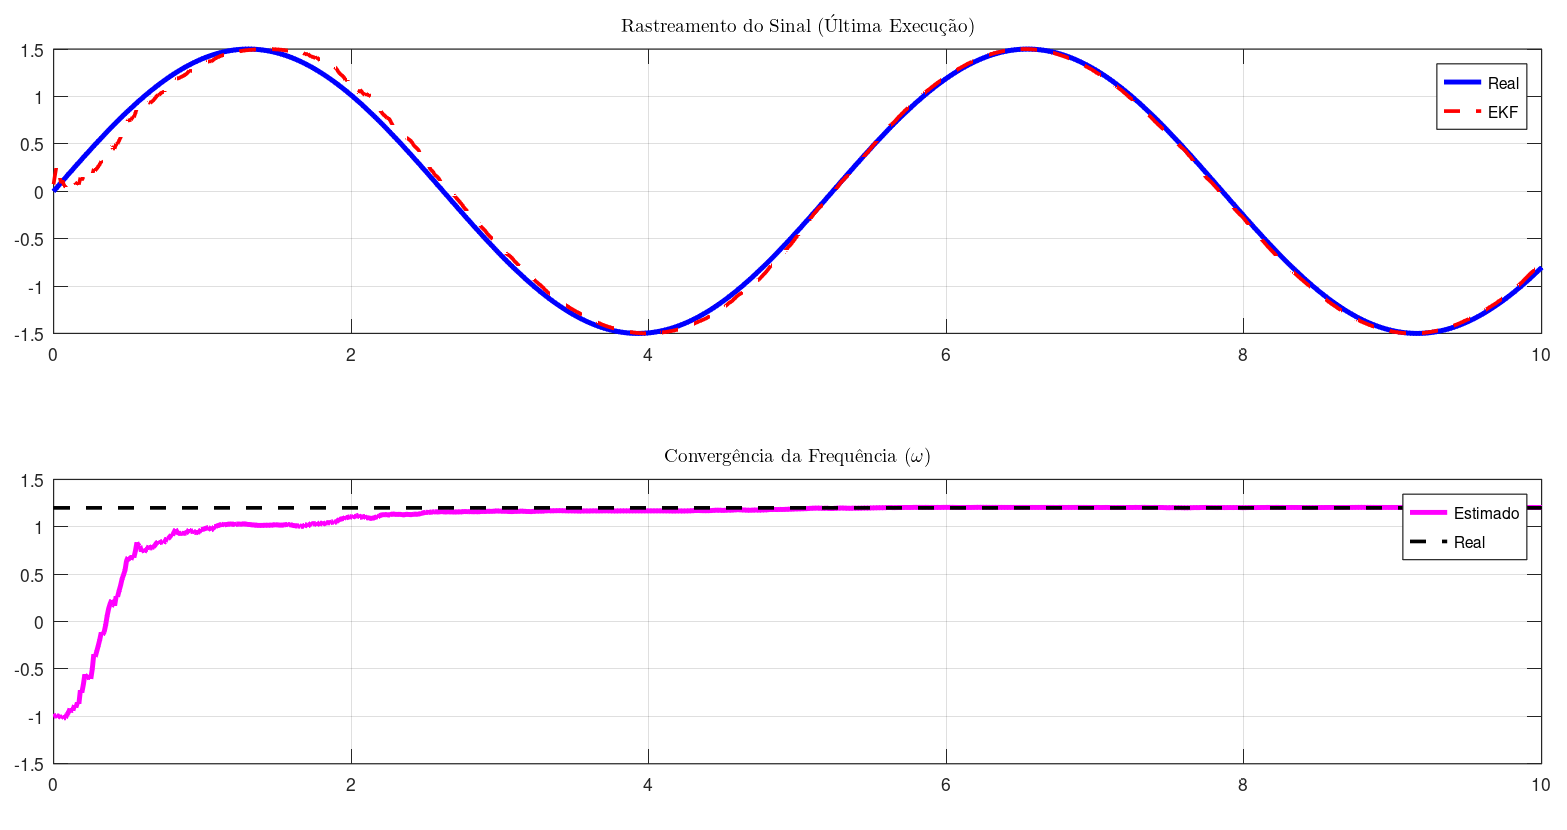
\includegraphics[width=12cm]{Figuras/modelo3/M3T2-GE.png}
    \label{fig:M3T2G}
    \caption*{\footnotesize \textbf{Fonte:} Elaborado pelo Autor (2026).}
\end{figure}

\begin{figure}[H]
    \centering
    \caption{Modelo 3: Convergências do erro (Teste 2).}
    \begin{minipage}{0.48\textwidth}
        \centering
        \caption*{\footnotesize \textbf{(a) MSE dos Estados ($\phi, \omega$)}}
        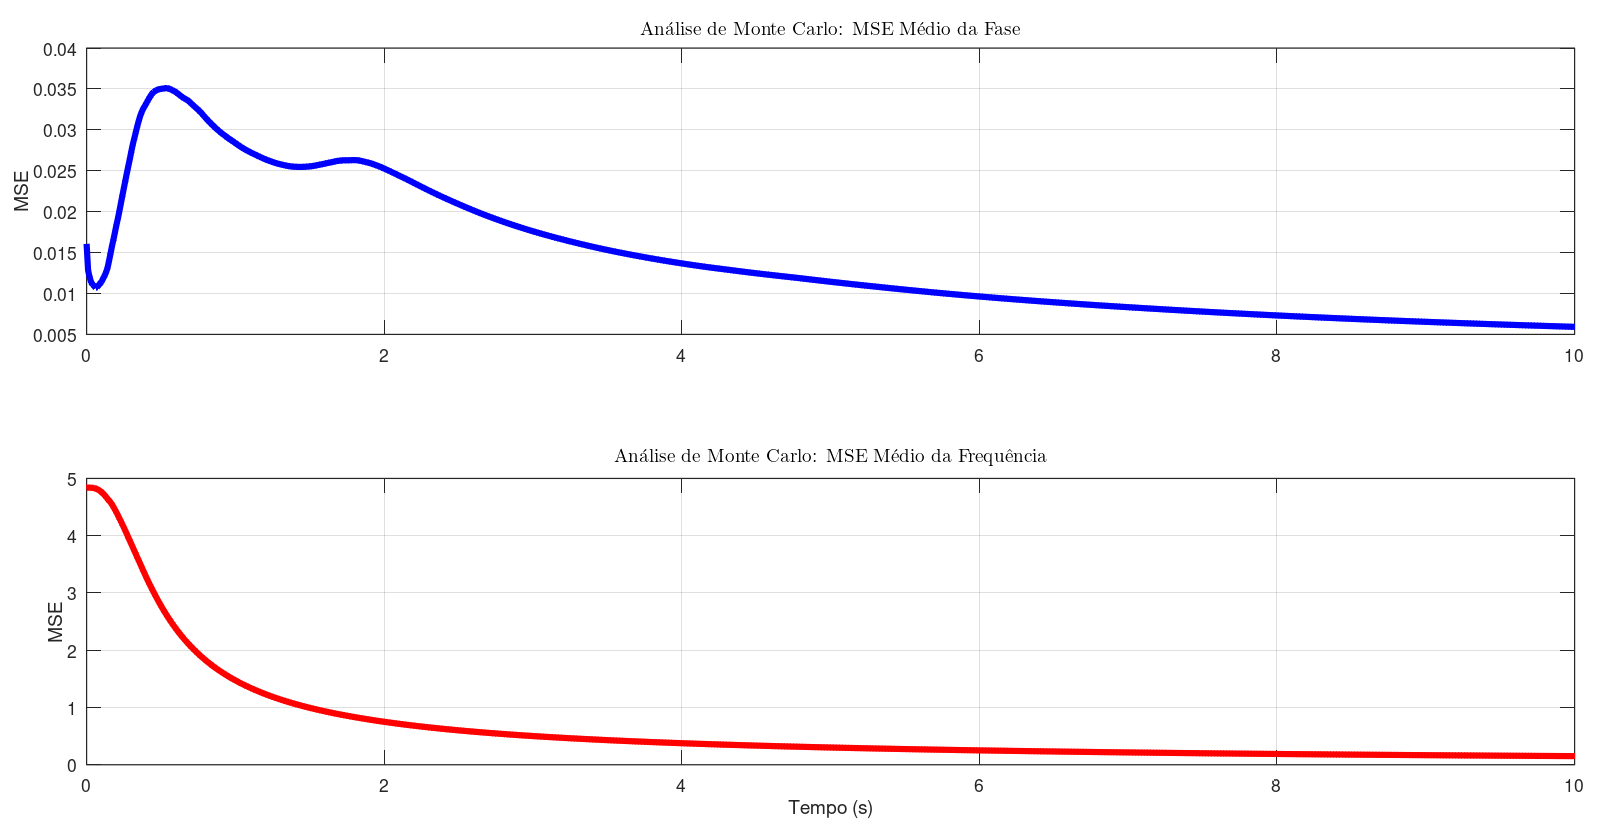
\includegraphics[width=\textwidth]{Figuras/modelo3/M3T2-GER.png}
    \end{minipage}\hfill
    \begin{minipage}{0.48\textwidth}
        \centering
        \caption*{\footnotesize \textbf{(b) MSE de Saída (Monta Carlo)}}
        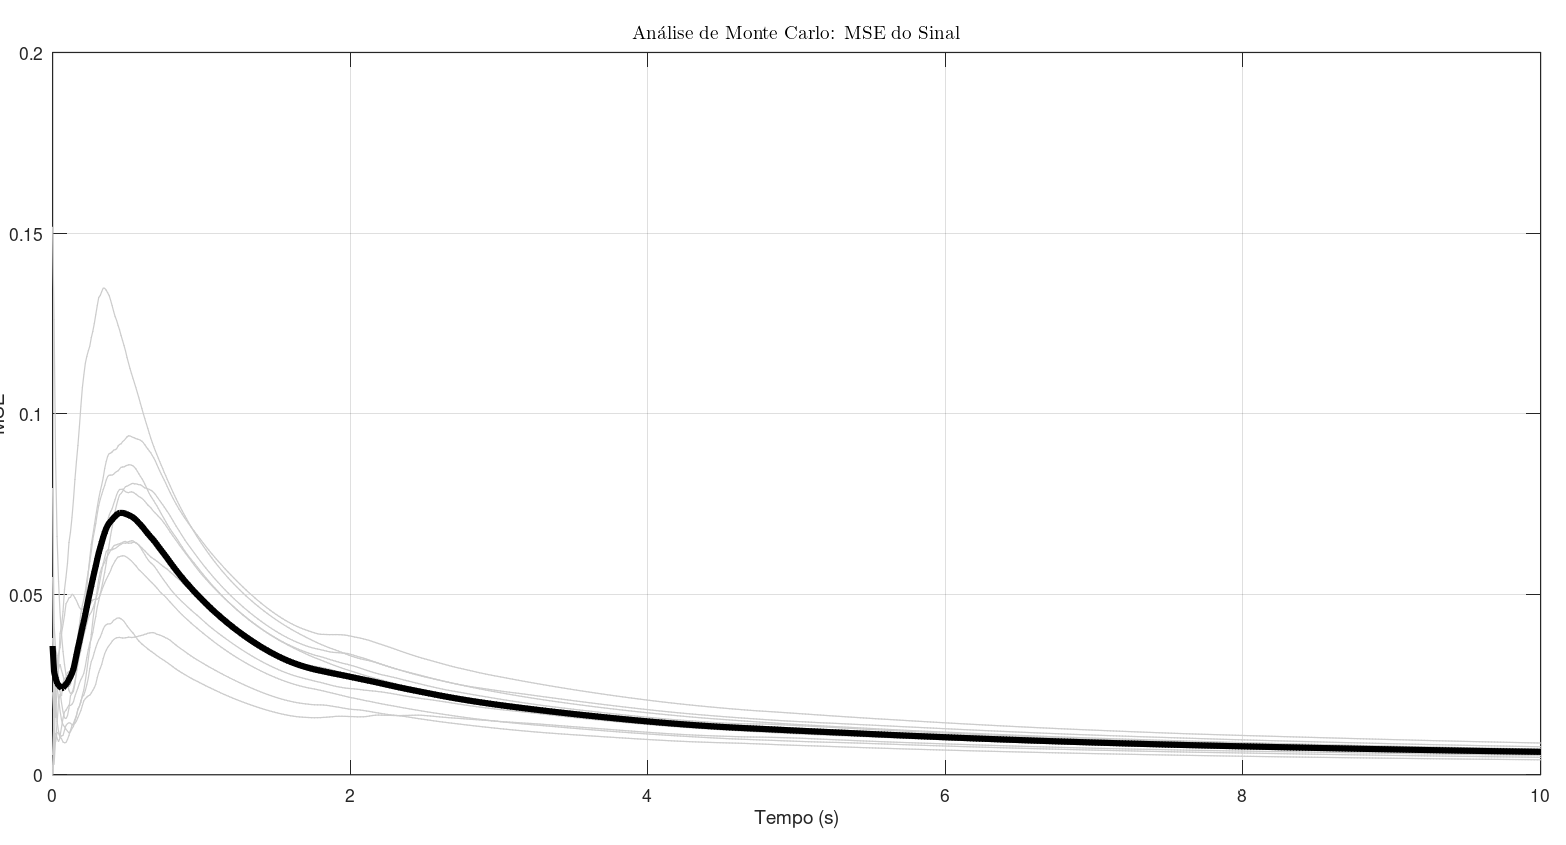
\includegraphics[width=\textwidth]{Figuras/modelo3/M3T2-GEER.png}
    \end{minipage}
    \caption*{\footnotesize \textbf{Fonte:} Elaborado pelo Autor (2026).}
    \label{fig:M3T2CONV_CO}
\end{figure}

\subsubsection{Teste 3: Convergência em Condições de Desajuste Acentuado}
\label{subsubsec:m3_teste3}

Os resultados do Teste 3 ratificam a superioridade do Modelo 3 no que tange à resposta em regime transiente. Observa-se uma redução significativa no tempo de acomodação da frequência angular ($\omega$) em comparação às arquiteturas precedentes, mesmo sob condições de severo desajuste inicial. A estabilidade do rastreamento, evidenciada na Figura \ref{fig:M3T3G}, sugere que a redução da ordem do vetor de estados mitiga a propagação de incertezas espúrias através das Jacobianas de predição, conferindo maior robustez ao algoritmo.

A análise das curvas de erro na Figura \ref{fig:M3T3CONV_CO} revela que a minimização do Erro Quadrático Médio (MSE) ocorre de forma assintótica e suave, apresentando um \textit{overshoot} desprezível nas estimativas de estado. Este fenômeno valida a hipótese de que, ao tratar a amplitude como um parâmetro invariante e conhecido, o filtro elimina um grau de liberdade não linear crítico. Consequentemente, o esforço computacional do EKF é concentrado na convergência da dinâmica temporal (frequência e fase), resultando em uma estimativa mais precisa e menos suscetível a instabilidades numéricas inerentes a modelos de maior dimensionalidade.

\begin{figure}[H]
    \centering
    \caption{Modelo 3: Estimativas (Teste 3).}
    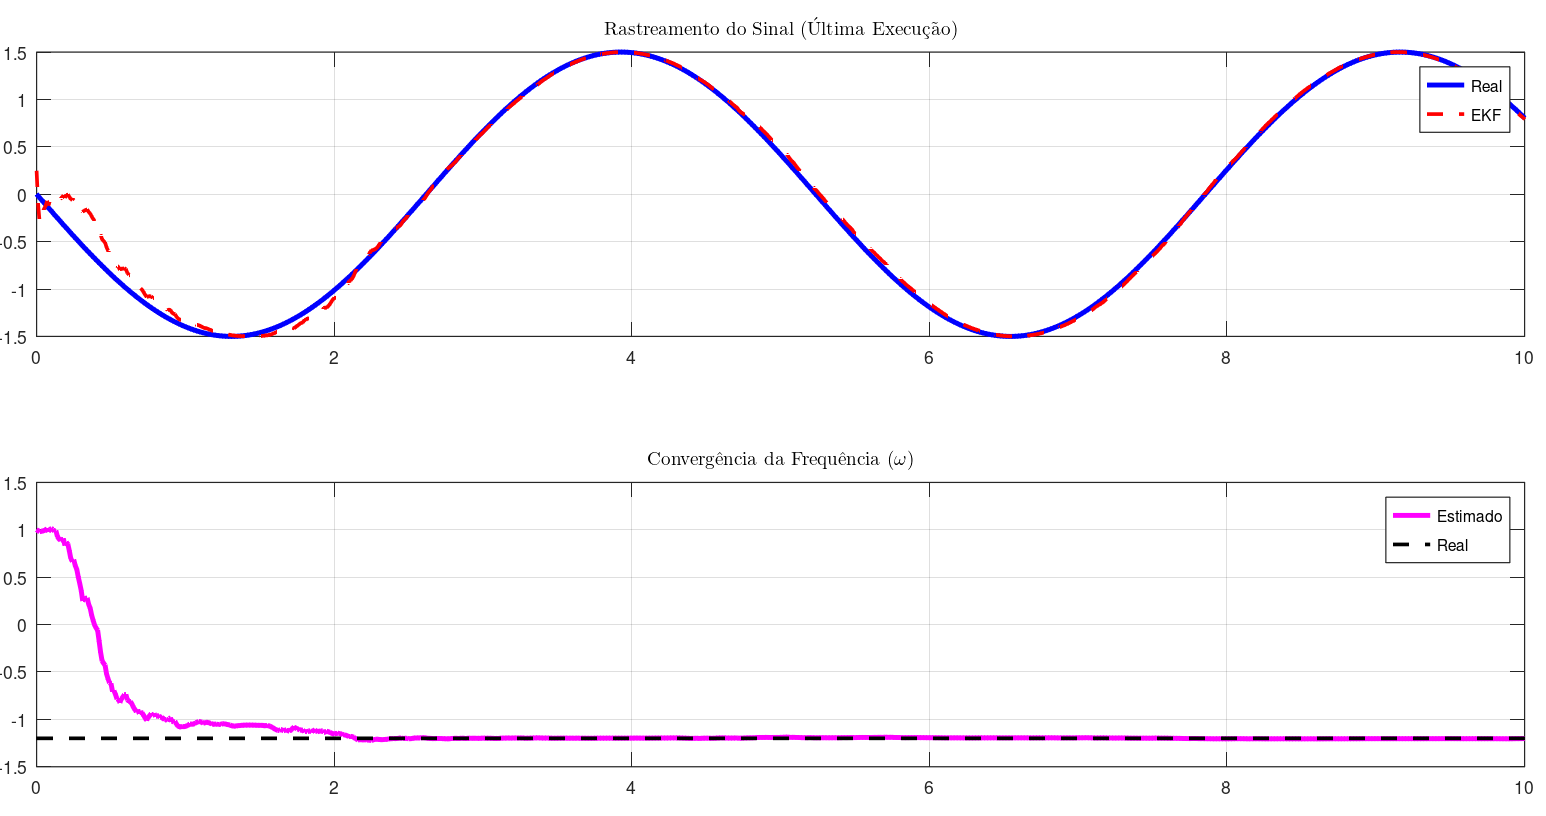
\includegraphics[width=14cm]{Figuras/modelo3/M3T3-GE.png}
    \label{fig:M3T3G}
    \caption*{\footnotesize \textbf{Fonte:} Elaborado pelo Autor (2026).}
\end{figure}

\begin{figure}[H]
    \centering
    \caption{Modelo 3: Convergências do erro (Teste 3).}
    \begin{minipage}{0.48\textwidth}
        \centering
         \caption*{\footnotesize \textbf{(a) MSE dos Estados ($\phi, \omega$)}}
        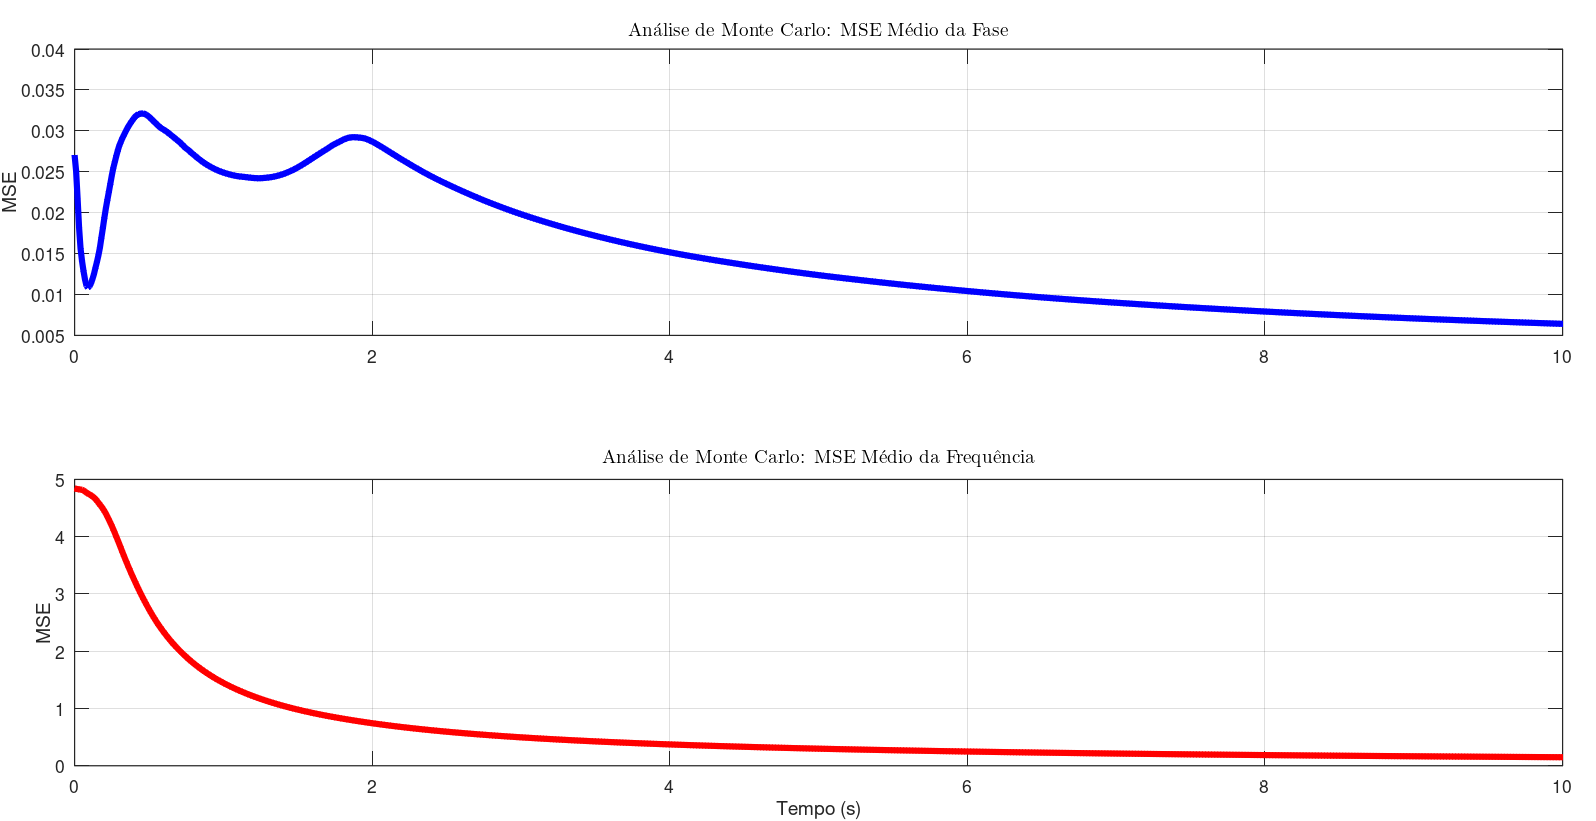
\includegraphics[width=\textwidth]{Figuras/modelo3/M3T3-GER.png}
    \end{minipage}\hfill
    \begin{minipage}{0.48\textwidth}
        \centering
        \caption*{\footnotesize \textbf{(b) MSE de Saída (Monta Carlo)}}
        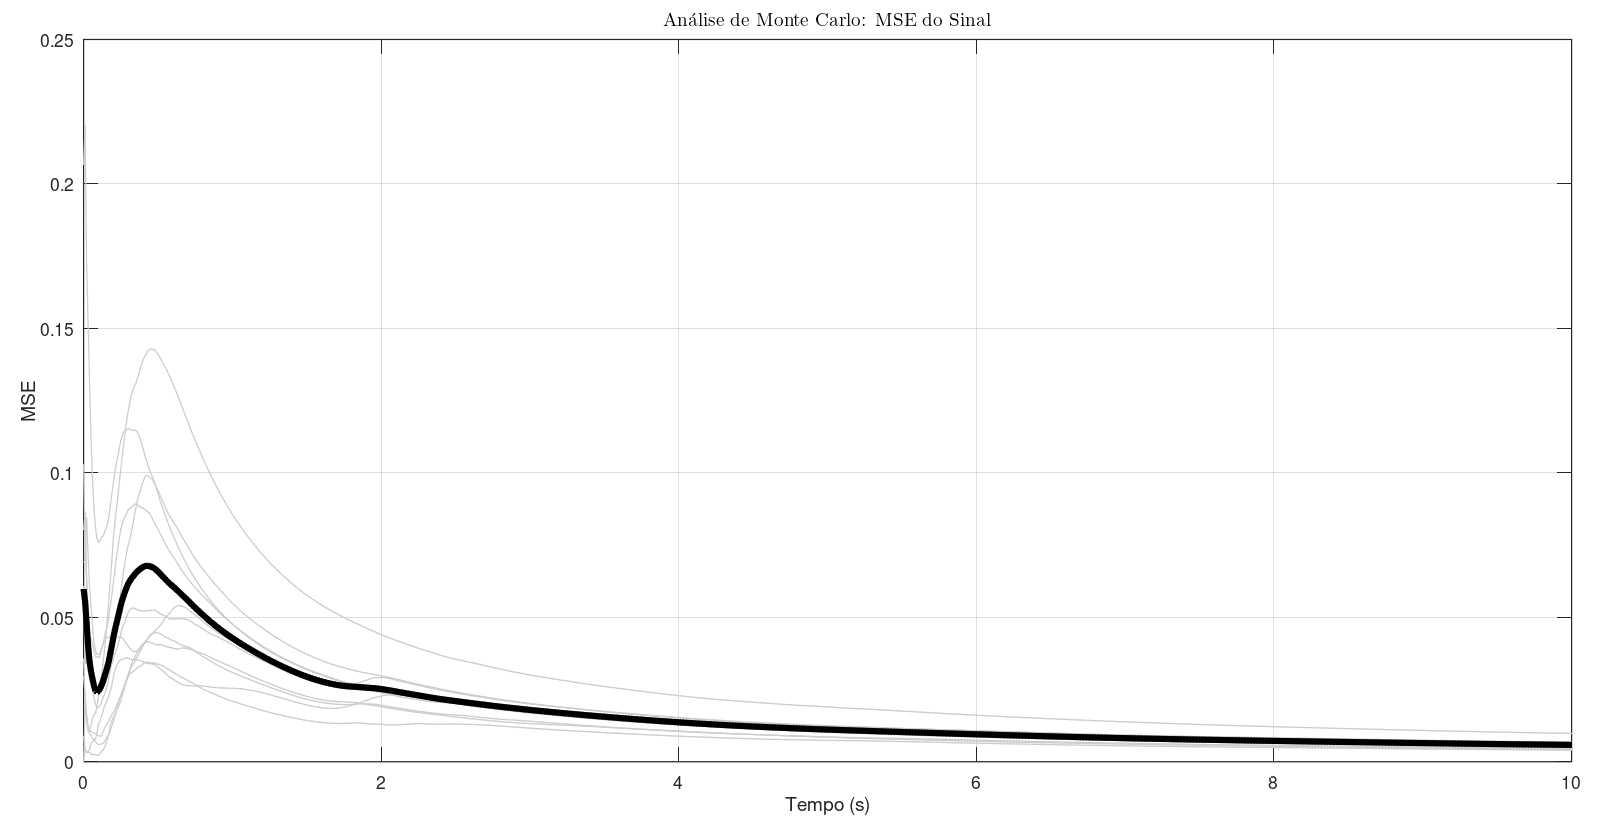
\includegraphics[width=\textwidth]{Figuras/modelo3/M3T3-GEER.png}
    \end{minipage}
    \caption*{\footnotesize \textbf{Fonte:} Elaborado pelo Autor (2026).}
    \label{fig:M3T3CONV_CO}
\end{figure}

\subsubsection{Conclusão Parcial do Modelo 3}
\label{subsubsec:discussao_m3}

Os resultados do Teste 3 ratificam a superioridade do Modelo 3 no que tange à resposta em regime transiente. Observa-se uma redução significativa no tempo de acomodação da frequência angular ($\omega$) em comparação às arquiteturas precedentes, mesmo sob condições de severo desajuste inicial. A estabilidade do rastreamento, evidenciada na Figura \ref{fig:M3T3G}, sugere que a redução da ordem do vetor de estados mitiga a propagação de incertezas espúrias através das Jacobianas de predição, conferindo maior robustez ao algoritmo.

A análise das curvas de erro na Figura \ref{fig:M3T3CONV_CO} revela que a minimização do Erro Quadrático Médio (MSE) ocorre de forma assintótica e suave, apresentando um \textit{overshoot} desprezível nas estimativas de estado. Este fenômeno valida a hipótese de que, ao tratar a amplitude como um parâmetro invariante e conhecido, o filtro elimina um grau de liberdade não linear crítico. Consequentemente, o esforço computacional do EKF é concentrado na convergência da dinâmica temporal (frequência e fase), resultando em uma estimativa mais precisa e menos suscetível a instabilidades numéricas inerentes a modelos de maior dimensionalidade.

\subsection{Análise do Modelo 4: Estados Dinâmicos $(x, \dot{x}, \omega)$}
\label{subsec:resultados_mod4}

Foram realizadas 10 repetições independentes (Monte Carlo) para cada configuração de teste. As figuras apresentadas nas subseções ilustram a décima execução como exemplo; nos gráficos de Monte Carlo a curva preta representa a média das 10 execuções e as curvas em tons de cinza representam as execuções individuais.

Para o modelo 4 (modelado na Subseção \ref{subsubsec:modelo4}), a transição para coordenadas dinâmicas (posição e velocidade do oscilador) proporcionou um incremento significativo na estabilidade do rastreio em ambientes ruidosos. Nesta topologia, o filtro estima a frequência angular como um estado variante, porém fundamentado na equação diferencial $\ddot{x} + \omega^2 x = 0$. 

Os testes realizados nesse modelo estão definidos seguindo a Tabela \ref{tab:parametros_m4}.

\begin{table}[H]
\centering
\caption{Parâmetros de simulação para os testes do Modelo 4.}
\label{tab:parametros_m4}
\begin{tabular}{l|c|c|c}
\hline
\textbf{Parâmetro} & \textbf{Teste 1} & \textbf{Teste 2} & \textbf{Teste 3} \\ \hline
$T_s$ (Amostragem) & \multicolumn{3}{c}{0,01 segundos} \\
Tempo Total & \multicolumn{3}{c}{10 segundos} \\ 
Monte Carlo & \multicolumn{3}{c}{10 repetições} \\ 
Amplitude (A) & \multicolumn{3}{c}{1,5} \\ 
$\omega$ & \multicolumn{3}{c}{1,2 rad/s} \\ 
$\phi_0$ & \multicolumn{3}{c}{0 rad} \\ \hline
$\sigma^2_{w1}$, $\sigma^2_{w2}$, $\sigma^2_{w3}$ & 0,001; 0,001; 0,01 & 0,001; 0,001; 0,1 & 0,5; 0,5; 2,0 \\ 
$R$ (Medição) & 0,1 & 0,1 & 2,0 \\ 
$\hat{\mathbf{x}}_0$ (Inicial) & $[0; 1; 1]^T$ & $[0; 1; 1]^T$ & $[10; 10; 10]^T$ \\ \hline
\end{tabular}
\end{table}

\subsubsection{Teste 1: Desempenho em Cenário Nominal}
\label{subsubsec:m4_teste1}

No cenário nominal, o Modelo 4 apresenta oscilações transientes características nas estimativas da derivada ($\dot{y}$) e da frequência angular ($\omega$). Este fenômeno decorre do forte acoplamento dinâmico no vetor de estados: como a predição da velocidade depende da precisão instantânea da posição ($y$), qualquer erro residual na estimativa de amplitude propaga-se diretamente para $\dot{y}$, o que, por conseguinte, instabiliza temporariamente o cálculo de $\omega$ através da Jacobiana adaptativa.

Diferente dos modelos anteriores, a convergência aqui é um processo iterativo de ajuste mútuo entre as variáveis físicas. As Figuras \ref{fig:M4T1G} e \ref{fig:M4T1CONV_CO} ilustram este comportamento, demonstrando que, após o período de sincronismo inicial, o filtro estabiliza e o Erro Quadrático Médio (MSE) decai para níveis condizentes com o limite ótimo de filtragem, validando a formulação dinâmica do estimador.

\begin{figure}[H]
    \centering
    \caption{Modelo 4: Estimativas (Teste 1).}
    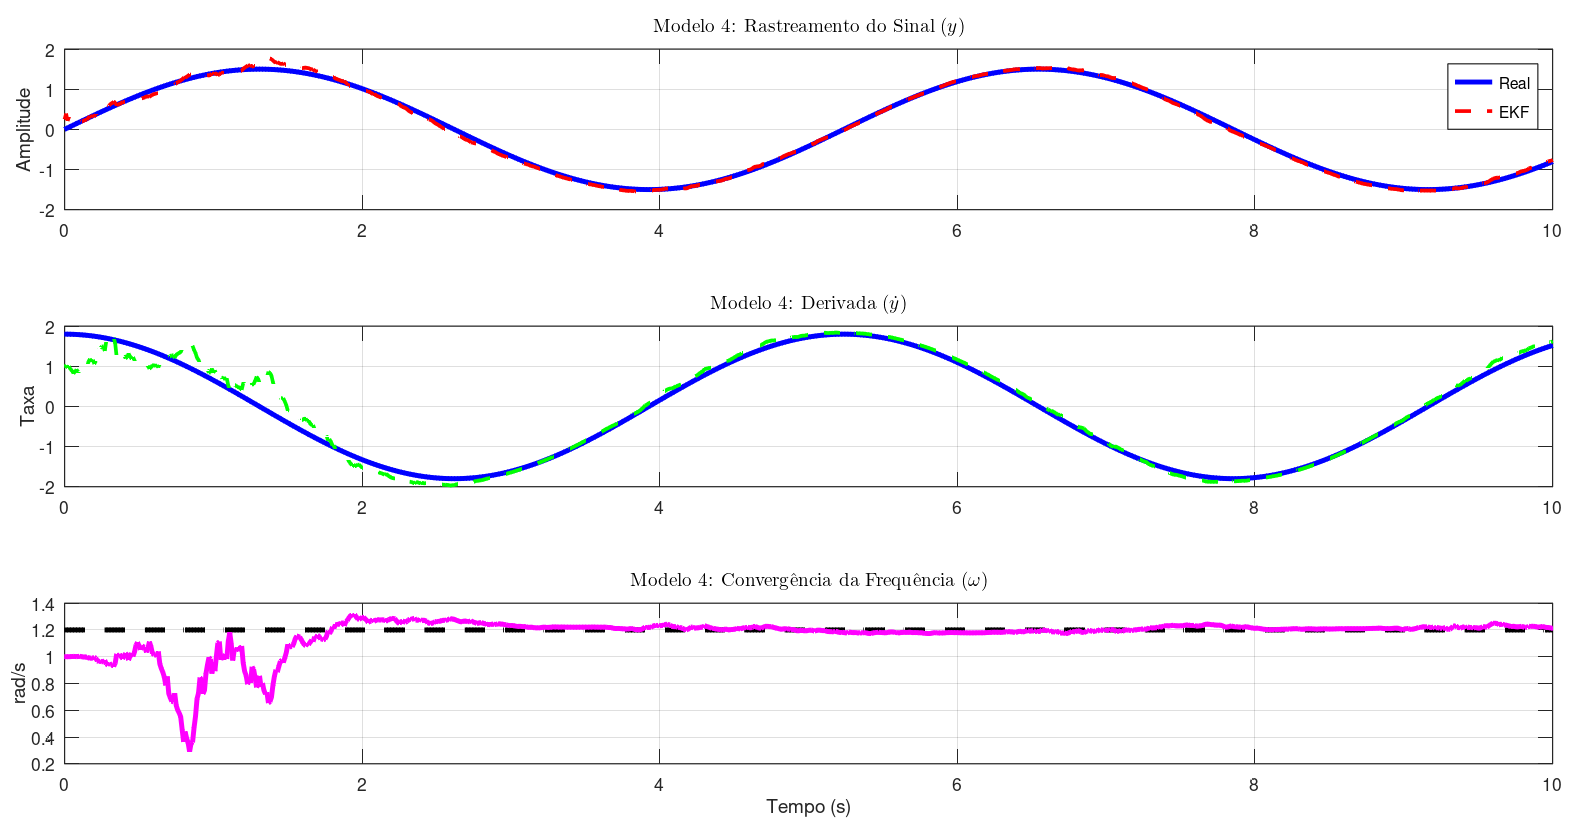
\includegraphics[width=14cm]{Figuras/modelo4/M4T1-GE.png}
    \label{fig:M4T1G}
    \caption*{\footnotesize \textbf{Fonte:} Elaborado pelo Autor (2026).}
\end{figure}

\begin{figure}[H]
    \centering
    \caption{Modelo 4: Convergências do erro (Teste 1).}
    \begin{minipage}{0.48\textwidth}
        \centering
        \caption*{\footnotesize \textbf{(a) MSE dos Estados $(x, \dot{x}, \omega)$}}
        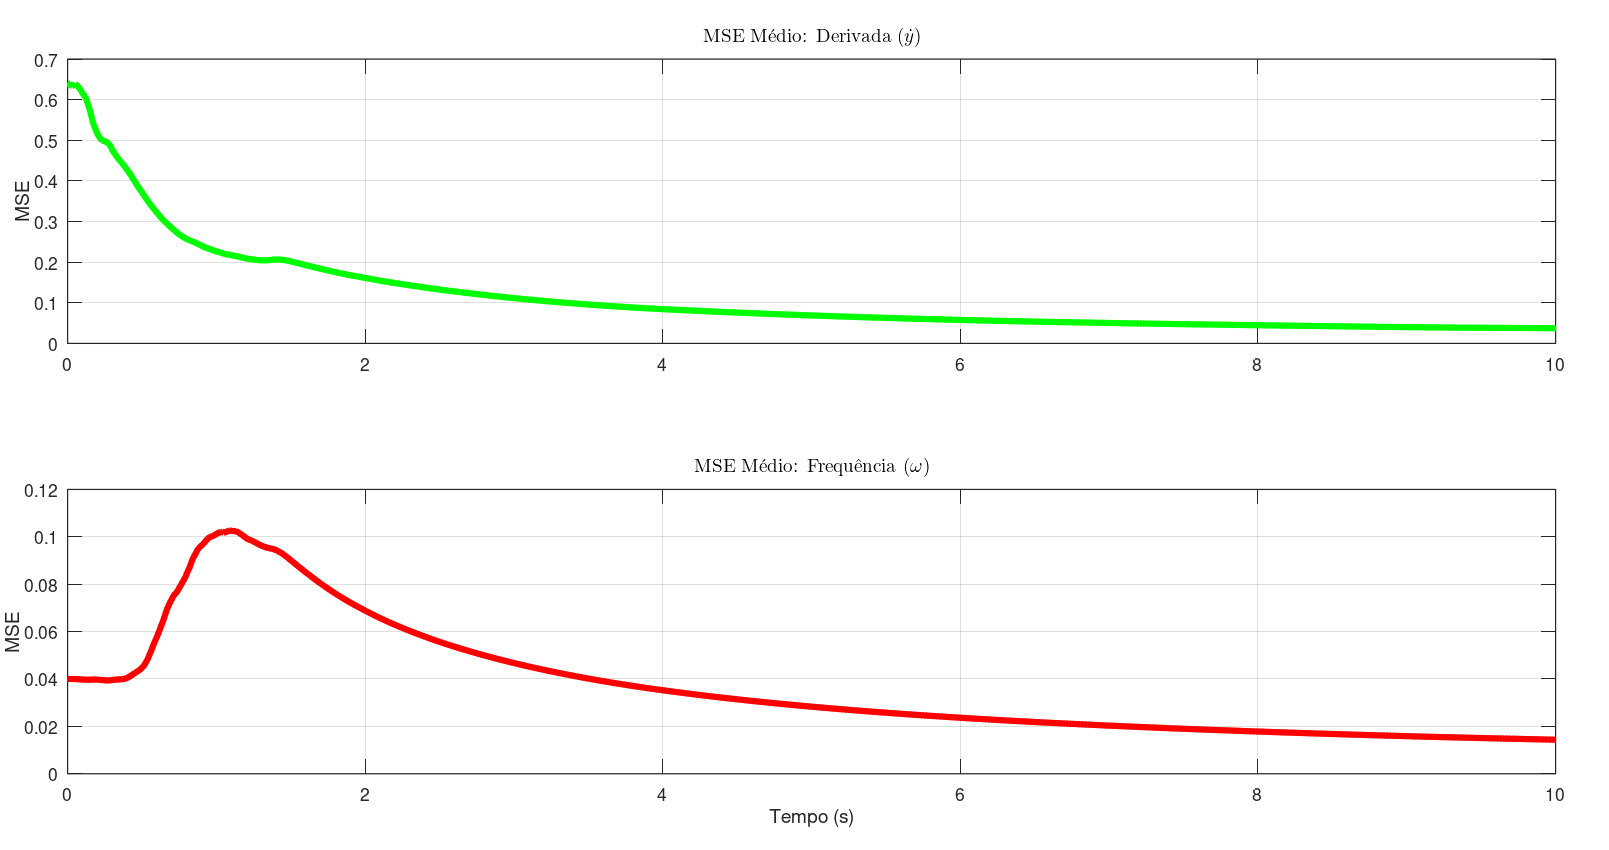
\includegraphics[width=\textwidth]{Figuras/modelo4/M4T1-GER.png}
    \end{minipage}\hfill
    \begin{minipage}{0.48\textwidth}
        \centering
        \caption*{\footnotesize \textbf{(b) MSE de saída (Monte Carlo)}}
        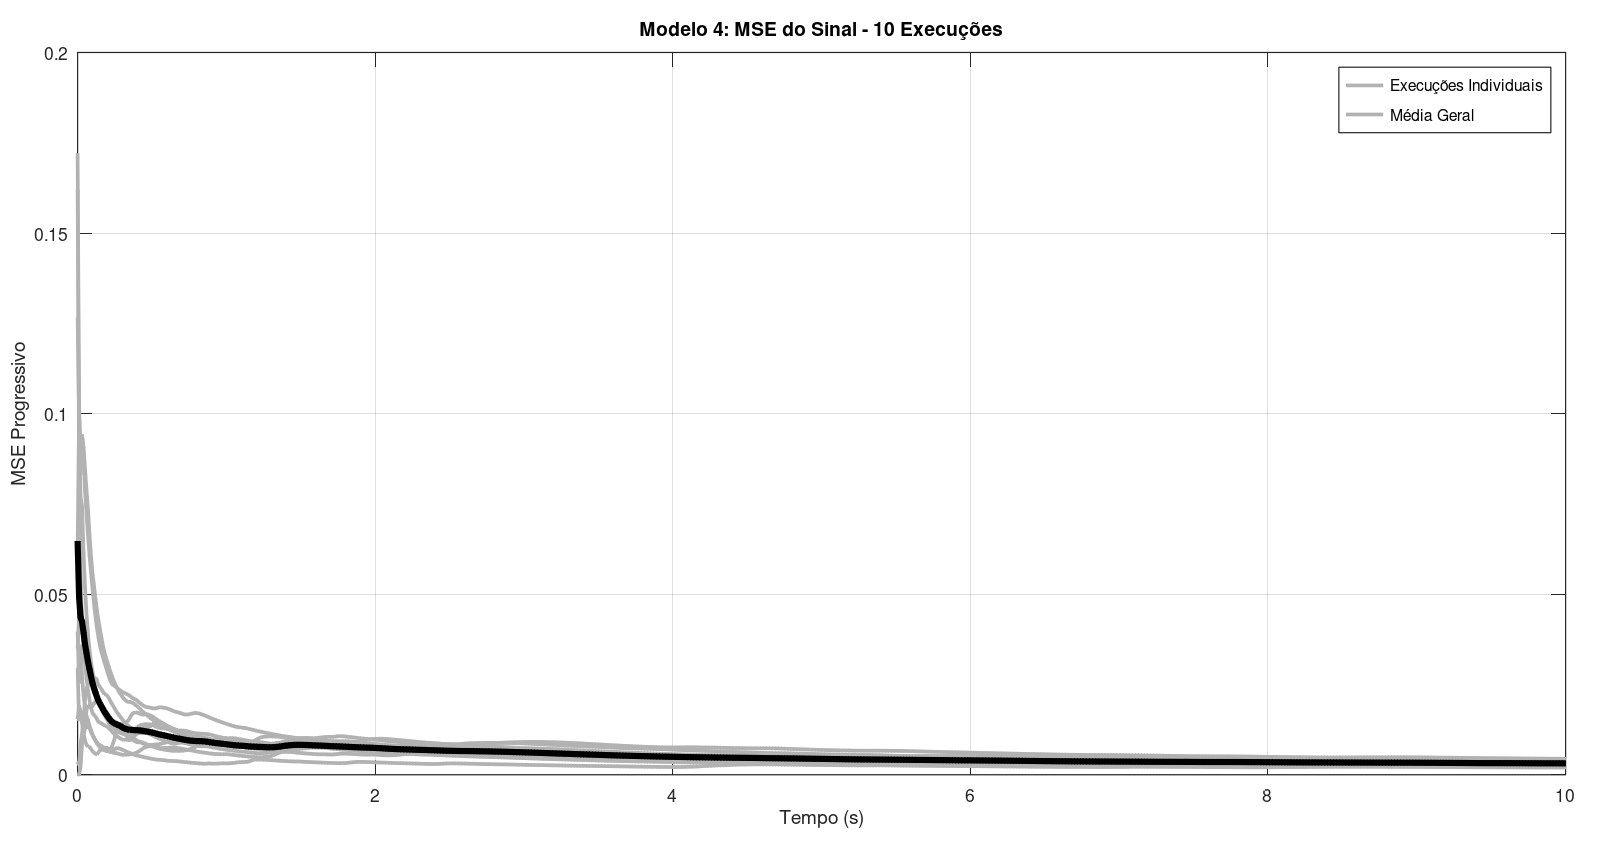
\includegraphics[width=\textwidth]{Figuras/modelo4/M4T1-GERR.png}
    \end{minipage}
    \label{fig:M4T1CONV_CO}
\end{figure}

\subsubsection{Teste 2: Resolução da Ambiguidade de Sinal}
\label{subsubsec:m4_teste2}

O \textbf{Teste 2} do Modelo 4 revela uma propriedade fundamental de sua formulação dinâmica: a invariância ao sinal da frequência angular inicial ($\hat{\omega}_0$). Ao inicializar o filtro com uma velocidade angular negativa, observa-se uma trajetória de convergência qualitativamente semelhante à do Teste 1. Este fenômeno ocorre porque a equação de transição de estados utiliza o termo quadrático da frequência ($\omega^2$) para definir a aceleração do sistema ($\ddot{y} = -\omega^2 y$).

Matematicamente, a função de custo do filtro não diferencia sinais opostos de $\omega$, uma vez que ambos produzem a mesma dinâmica de oscilação para o sinal $y$. Consequentemente, o modelo converge para o \textit{mínimo quadrático} mais próximo da estimativa inicial, validando a estabilidade do Modelo 4 mesmo em cenários de incerteza de fase ou direção rotacional. Esta característica torna o Modelo 4 superior ao Modelo 2, pois elimina a necessidade de inversão da amplitude ou deslocamentos espúrios de fase para compensar o sinal da frequência.

\begin{figure}[H]
    \centering
    \caption{Modelo 4: Estimativas (Teste 2).}
    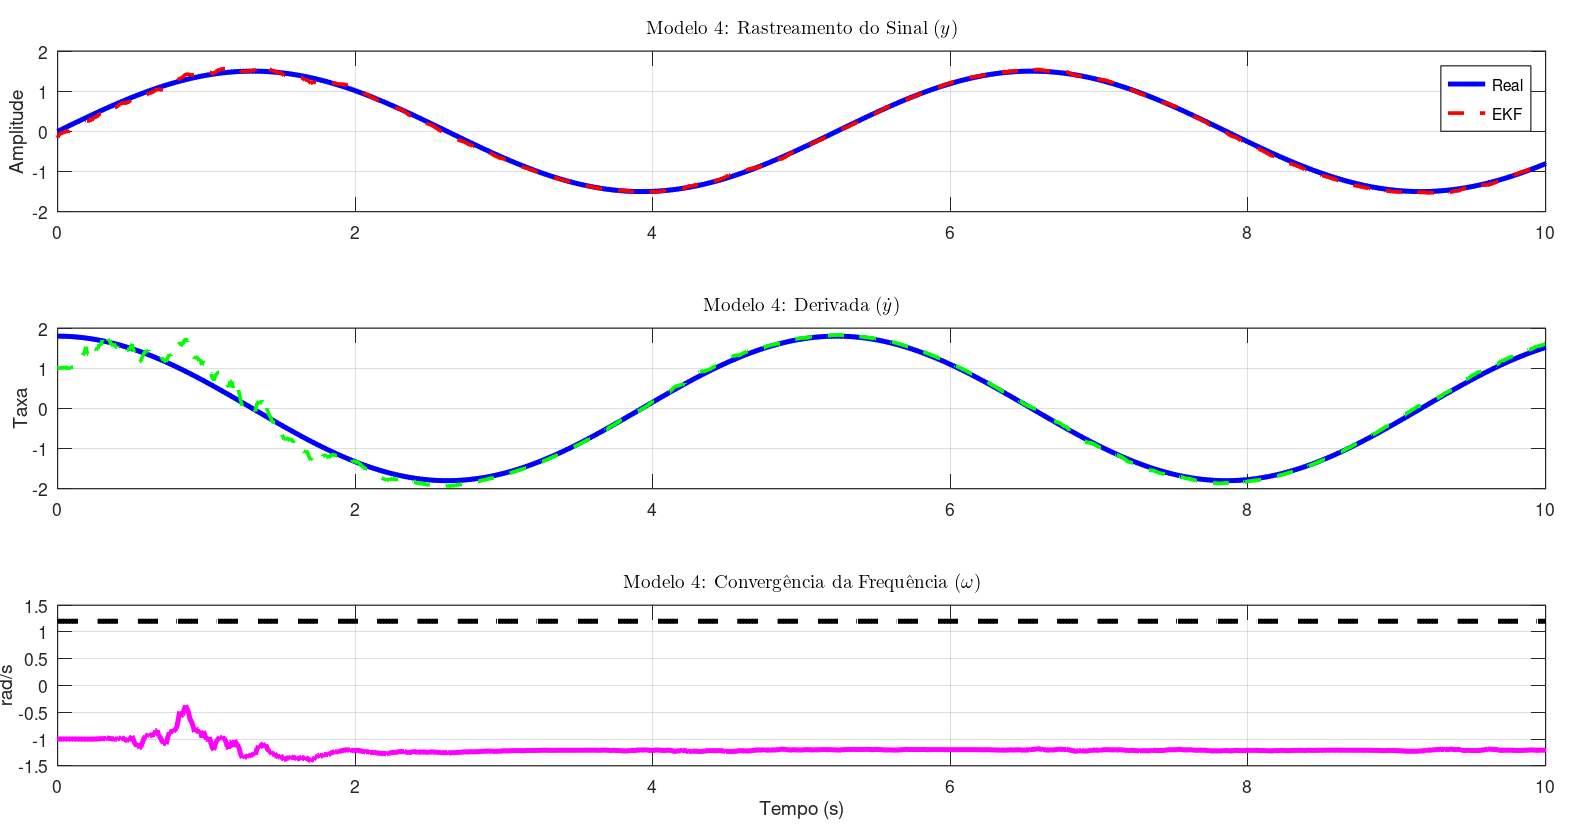
\includegraphics[width=14cm]{Figuras/modelo4/M4T2-GE.png}
    \label{fig:M4T2G}
    \caption*{\footnotesize \textbf{Fonte:} Elaborado pelo Autor (2026).}
\end{figure}

\begin{figure}[H]
    \centering
    \caption{Modelo 4: Convergências do erro (Teste 2).}
    \begin{minipage}{0.48\textwidth}
        \centering
        \caption*{\footnotesize \textbf{(a) MSE dos Estados $(x, \dot{x}, \omega)$}}
        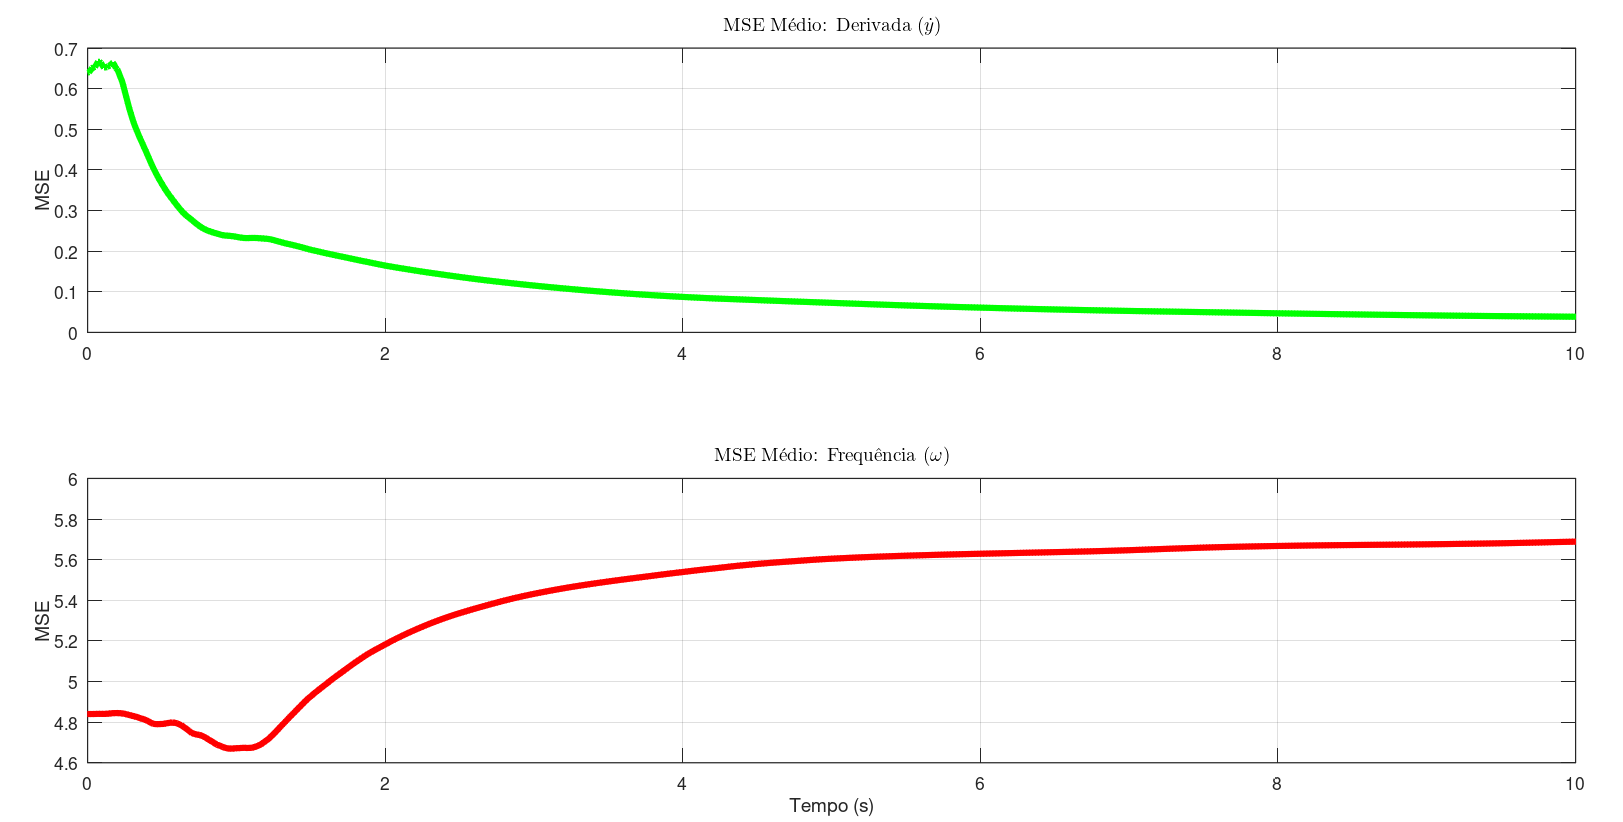
\includegraphics[width=\textwidth]{Figuras/modelo4/M4T2-GER.png}
    \end{minipage}\hfill
    \begin{minipage}{0.48\textwidth}
        \centering
        \caption*{\footnotesize \textbf{(b) MSE de saída (Monte Carlo)}}
        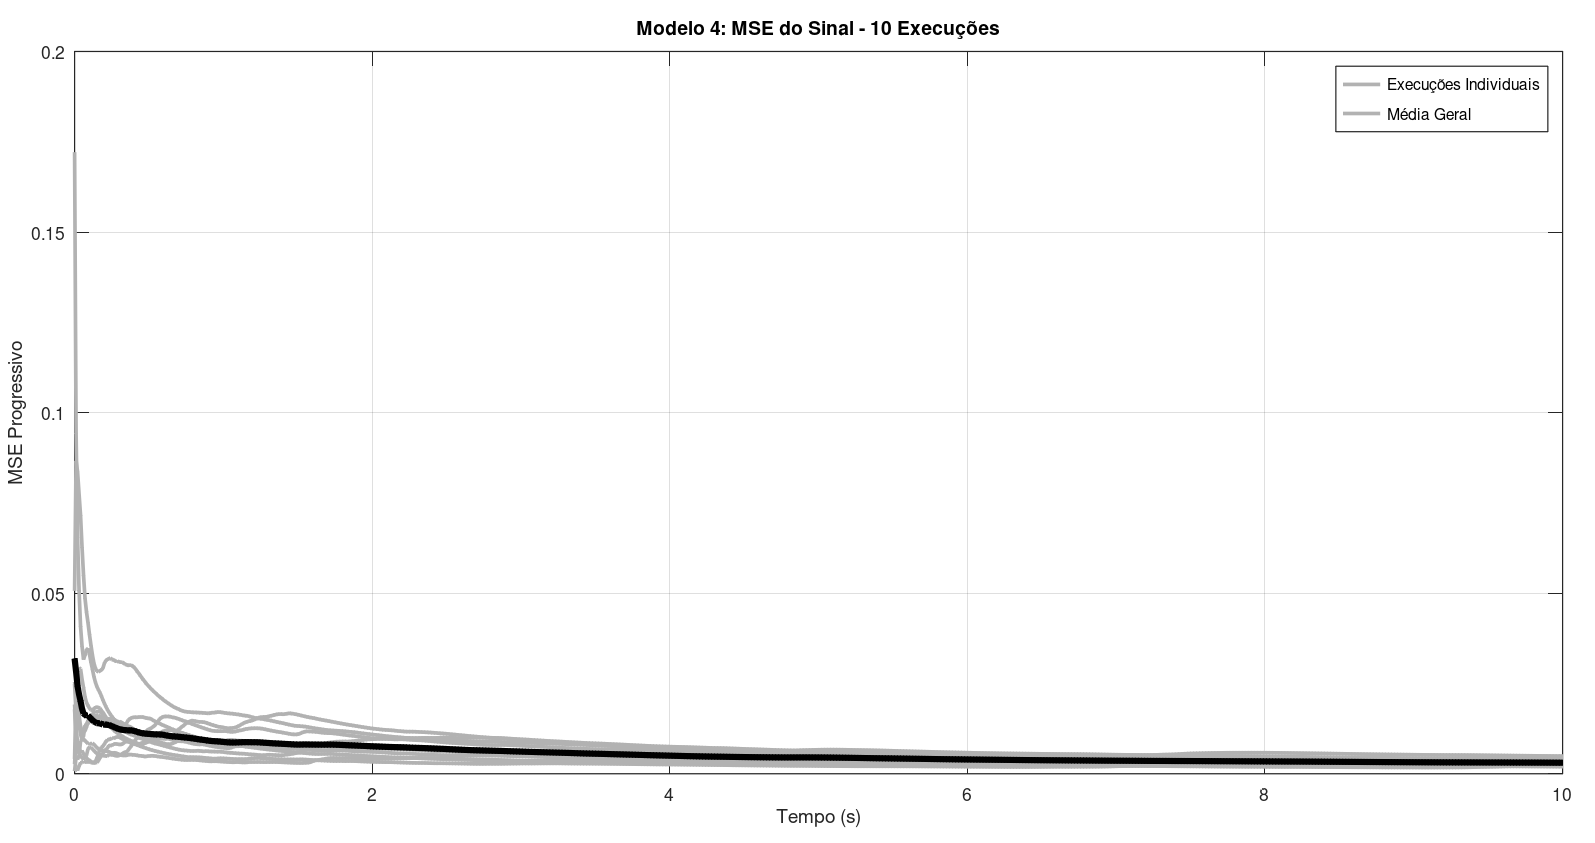
\includegraphics[width=\textwidth]{Figuras/modelo4/M4T2-GEER.png}
    \end{minipage}
    \caption*{\footnotesize \textbf{Fonte:} Elaborado pelo Autor (2026).}
    \label{fig:M4T2CONV_CO}
\end{figure}

\subsubsection{Teste 3: Robustez à Estimativa Inicial e Transiente de Adaptação}
\label{subsubsec:m4_teste3}

O \textbf{Teste 3} avalia o comportamento do Modelo 4 sob condições de forte desajuste entre a estimativa inicial e os parâmetros reais do sistema. Observa-se que o filtro mantém uma instabilidade característica nas estimativas de velocidade ($\dot{y}$) e frequência angular ($\omega$) durante o período inicial de operação. Este fenômeno é atribuído ao \textit{tempo de acomodação} do estimador, uma vez que as Jacobianas adaptativas dependem da convergência prévia do sinal de saída para linearizar corretamente a dinâmica do oscilador.

Contudo, um resultado de destaque deste modelo é sua capacidade de convergência acelerada: mesmo com valores iniciais significativamente distantes do regime nominal, o filtro atinge a estabilidade antes da conclusão de um ciclo completo da senoide ($t < 2\pi/\omega$). Este desempenho evidencia a robustez da formulação em variáveis de estado, que consegue reajustar o ganho de Kalman ($K$) de forma eficiente para corrigir o erro de fase e frequência de maneira simultânea, como ilustrado na Figura \ref{fig:M4T3G}.

\begin{figure}[H]
    \centering
    \caption{Modelo 4: Estimativas (Teste 3).}
    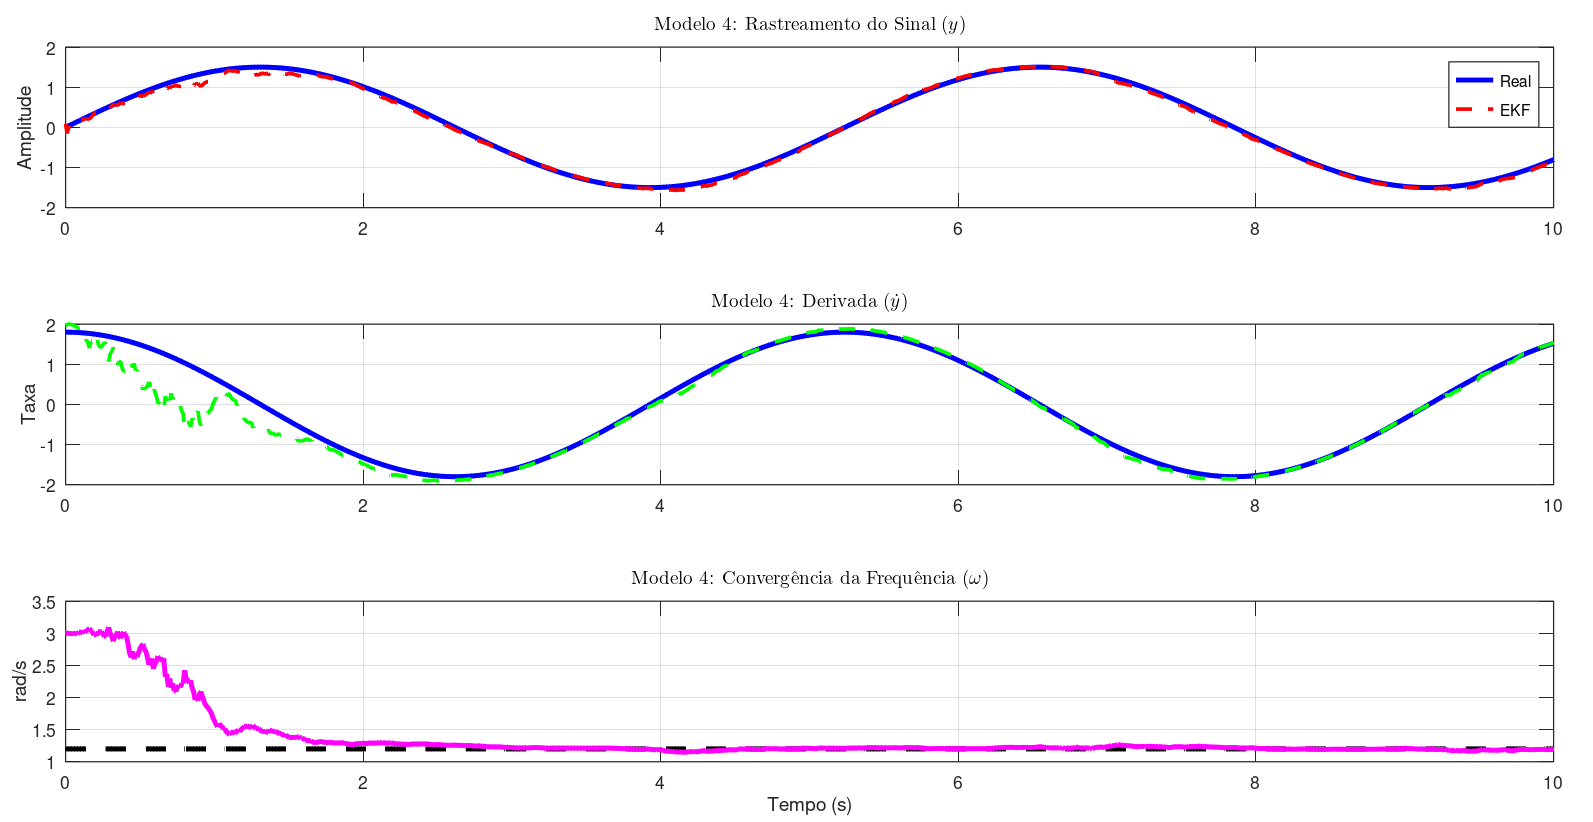
\includegraphics[width=14cm]{Figuras/modelo4/M4T3-GE.png}
    \label{fig:M4T3G}
    \caption*{\footnotesize \textbf{Fonte:} Elaborado pelo Autor (2026).}
\end{figure}

\begin{figure}[H]
    \centering
    \caption{Modelo 4: Convergências do erro (Teste 3).}
    \begin{minipage}{0.48\textwidth}
        \centering
        \caption*{\footnotesize \textbf{(a) MSE dos Estados $(x, \dot{x}, \omega)$}}
        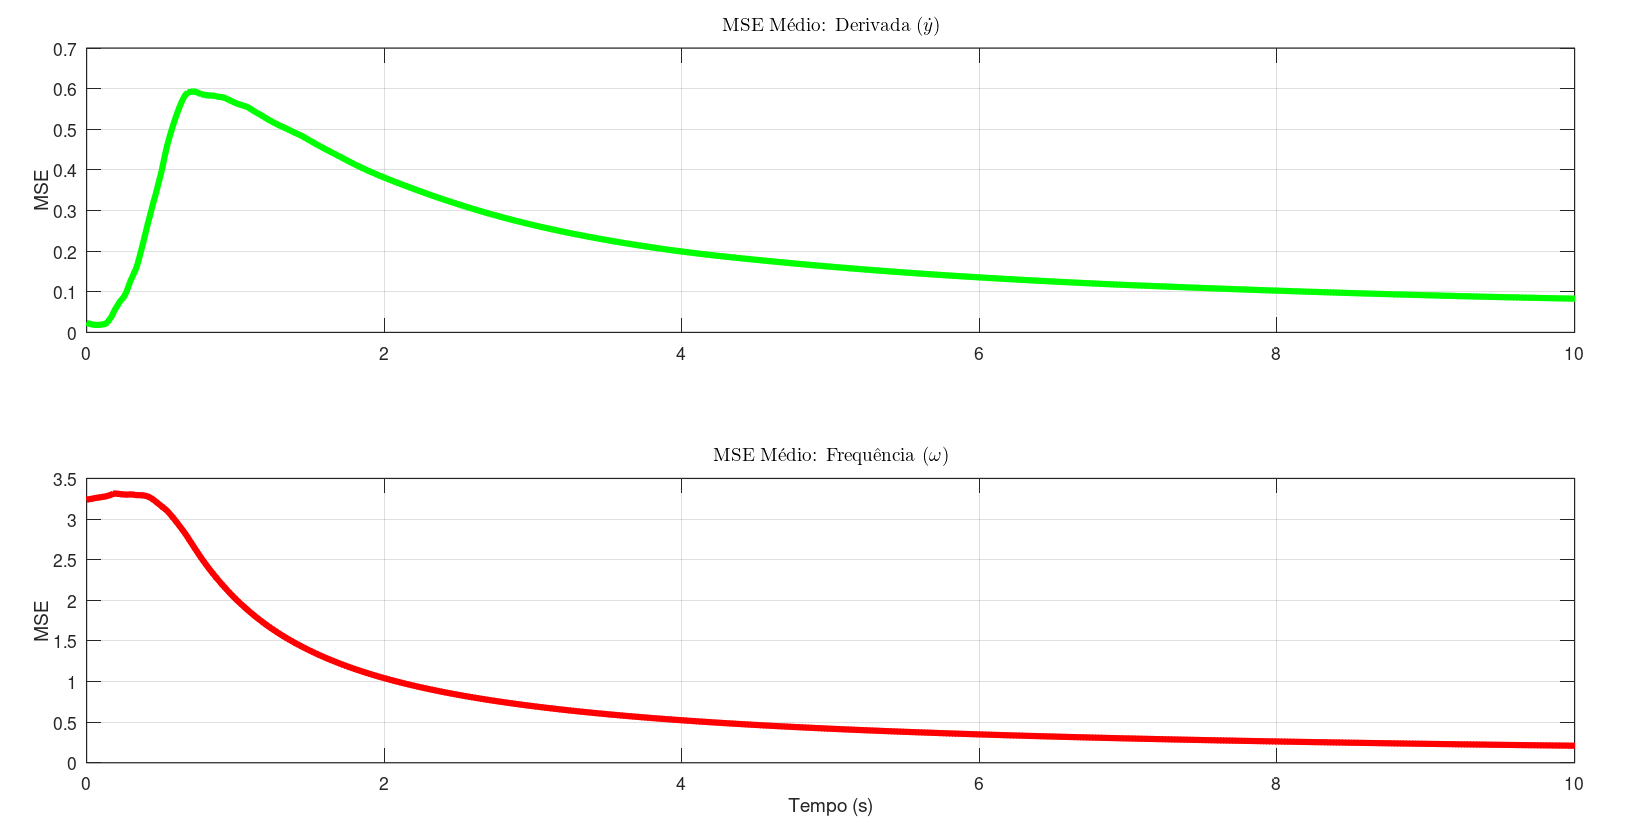
\includegraphics[width=\textwidth]{Figuras/modelo4/M4T3-GER.png}
    \end{minipage}\hfill
    \begin{minipage}{0.48\textwidth}
        \centering
        \caption*{\footnotesize \textbf{(b) MSE de saída (Monte Carlo)}}
        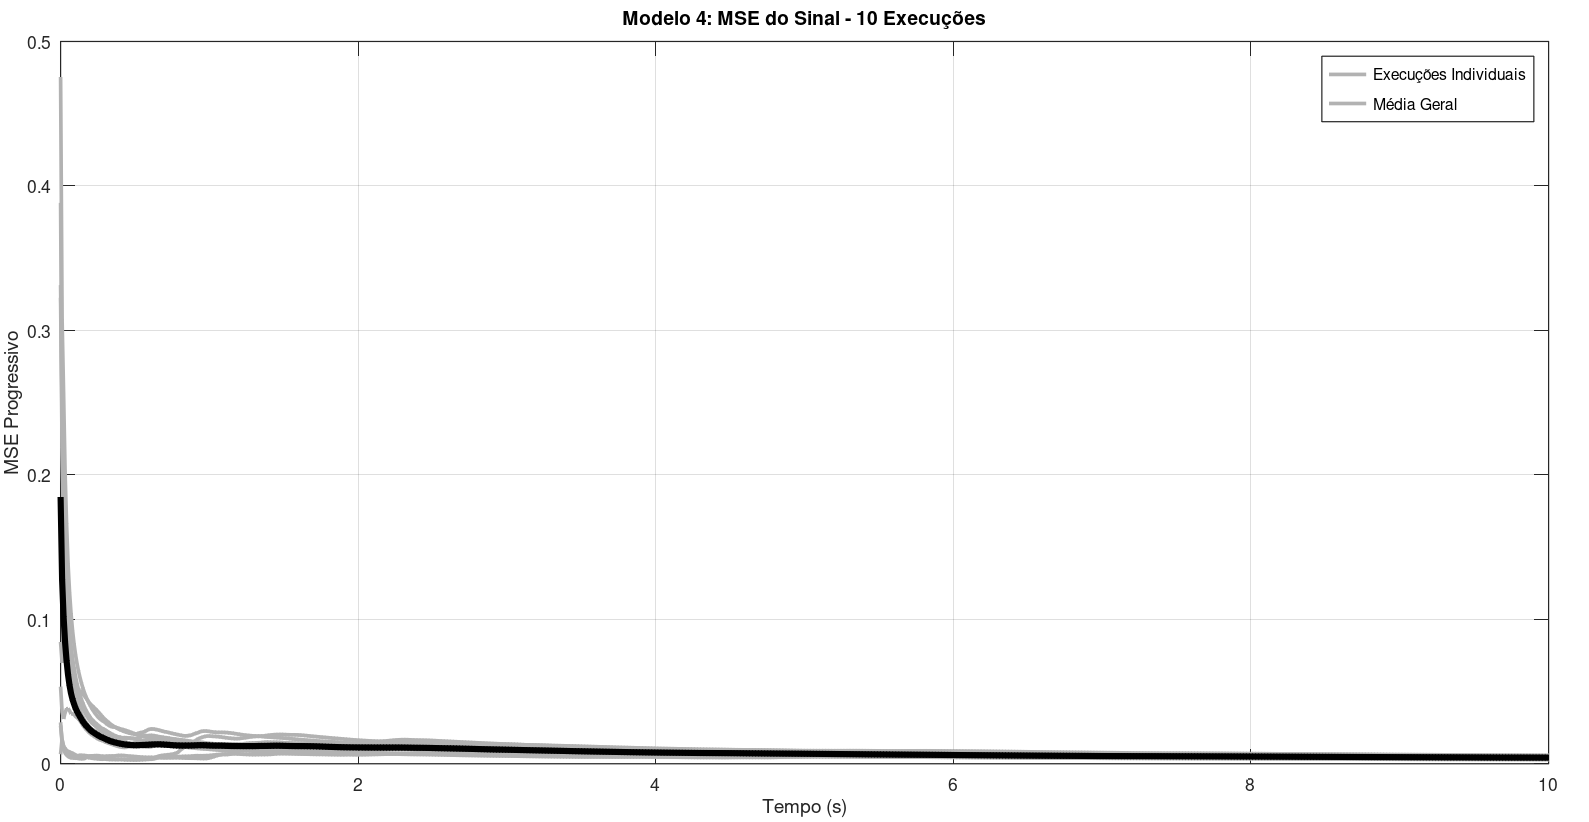
\includegraphics[width=\textwidth]{Figuras/modelo4/M4T3-GEER.png}
    \end{minipage}
    \caption*{\footnotesize \textbf{Fonte:} Elaborado pelo Autor (2026).}
    \label{fig:M4T3CONV_CO}
\end{figure}


\subsubsection{Conclusão da Parcial do Modelo 4}

O autor concluiu que o Modelo 4 é eficaz em estimar os estados da senoide de forma robusta frente à inicialização. Contudo, a estimação exata do sinal e do sinal da frequência depende da coincidência do sinal da estimativa inicial com o da frequência real; em casos de incompatibilidade, o filtro estima corretamente a magnitude de $\omega$ mas erra a polaridade, devido à presença do termo $\omega^2$ nas equações de estado. Ainda assim, para fins de rastreio do sinal e sua derivada, conhecer apenas a magnitude de $\omega$ é suficiente, tornando o modelo prático para aplicações onde o sinal da frequência não é crítico \cite{zarchan2015}.


\subsection{Análise do Modelo 5: Resolução via Frequência ao Quadrado ($x, \dot{x}, z$)}
\label{subsec:resultados_mod5}

Foram realizadas 10 repetições independentes (Monte Carlo) para cada configuração de teste. As figuras apresentadas nas subseções ilustram a décima execução como exemplo; nos gráficos de Monte Carlo a curva preta representa a média das 10 execuções e as curvas em tons de cinza representam as execuções individuais.

O Modelo 5 (modelado na Subseção \ref{subsubsec:modelo5}) representa a solução definitiva para os problemas de ambiguidade encontrados nas versões anteriores. Ao redefinir o terceiro estado como o quadrado da frequência angular ($z = \omega^2$), a inobservabilidade do sinal é eliminada por construção matemática. Esta abordagem remove a não linearidade excessiva da função seno em relação à frequência, simplificando a superfície de erro do filtro.

\begin{table}[H]
\centering
\caption{Parâmetros de simulação para os testes do Modelo 5.}
\label{tab:parametros_m5}
\begin{tabular}{l|c|c|c}
\hline
\textbf{Parâmetro} & \textbf{Teste 1} & \textbf{Teste 2} & \textbf{Teste 3} \\ \hline
$T_s$ (Amostragem) & \multicolumn{3}{c}{0,01 segundos} \\
Tempo Total & \multicolumn{3}{c}{10 segundos} \\ 
Monte Carlo & \multicolumn{3}{c}{10 repetições} \\ 
Amplitude (A) & \multicolumn{3}{c}{1.5} \\ 
$\omega$ & \multicolumn{3}{c}{1.2 rad/s} \\ 
$\phi_0$ & \multicolumn{3}{c}{0 rad} \\ \hline
$\sigma^2_{w1}, \sigma^2_{w2}, \sigma^2_{w3}$ & 0,001; 0,001; 0,01 & 0,001; 0,001; 0,1 & 0,5; 0,5; 2,0 \\ 
$R$ (Medição) & 0,1 & 0,1 & 2,0 \\ 
$\hat{\mathbf{x}}_0$ (Inicial) & $[0; 1; 1]^T$ & $[0; 1; -1]^T$ & $[10; 10; -10]^T$ \\ \hline
\end{tabular}
\end{table}

\subsubsection{Teste 1: Desempenho em Cenário Nominal}

No cenário nominal, o Modelo 5 demonstrou uma convergência rápida e estável para o sinal de saída, apresentando um desempenho comparável ao do Modelo 4. Adicionalmente, o rastreamento do estado correspondente à derivada do sinal ($\dot{y}$) ocorreu de forma célere e sem desvios abruptos. Embora o regime transiente ainda apresente oscilações na estimativa da frequência angular ($\omega$), nota-se que estas se manifestam com uma amplitude significativamente atenuada em relação à arquitetura anterior.

As Figuras \ref{fig:M5T2G} e \ref{fig:M5T2CONV_CO} ilustram o comportamento das estimativas de estado e a evolução da convergência do erro para o Teste 2.


\begin{figure}[H]
    \centering
    \caption{Modelo 5: Estimativas (Teste 1).}
    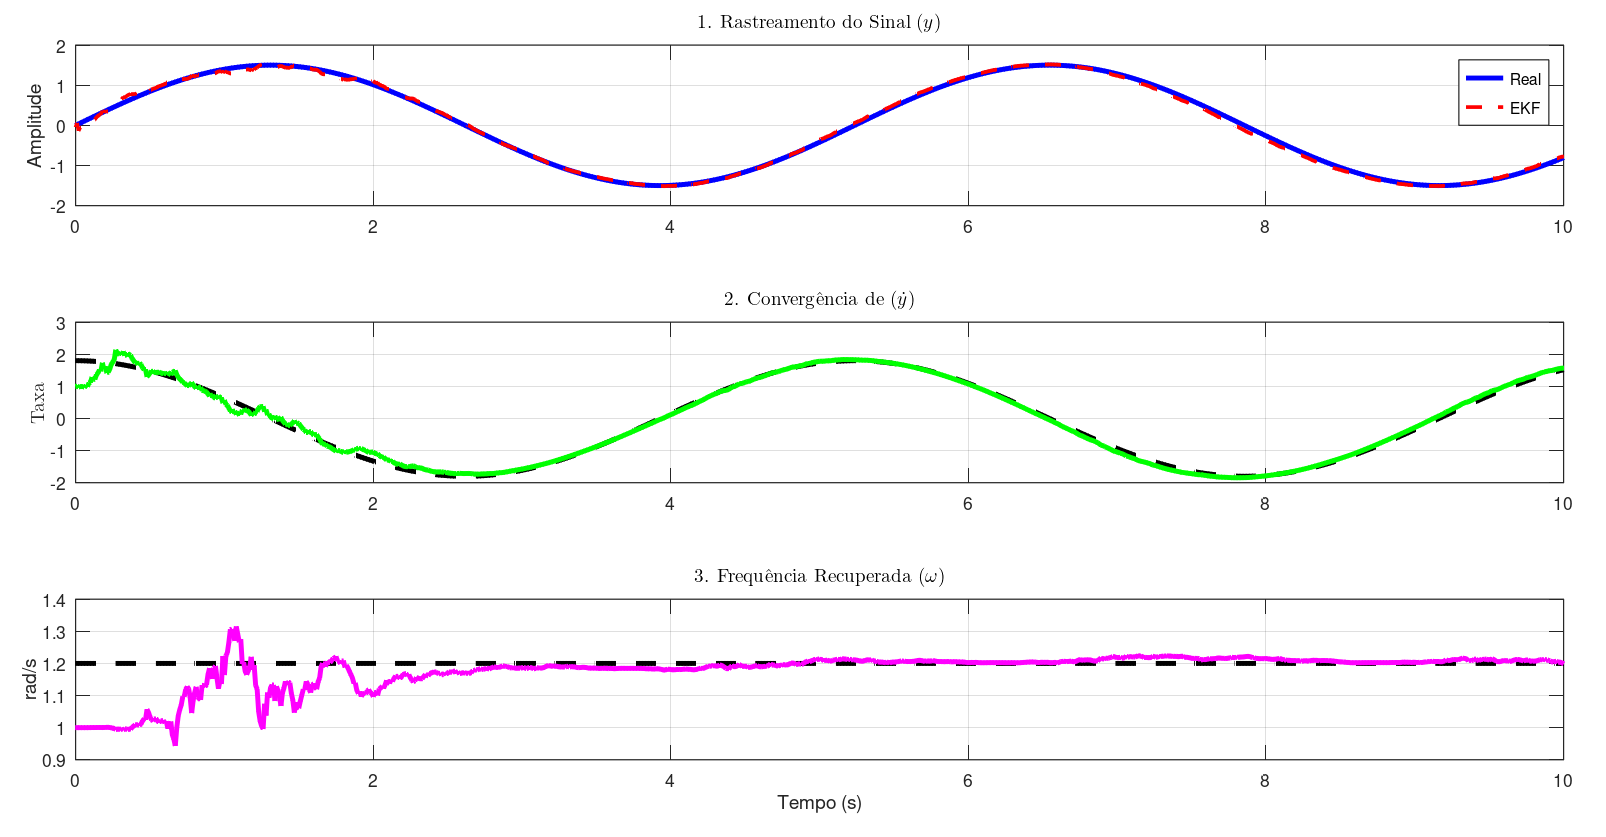
\includegraphics[width=14cm]{Figuras/modelo5/M5T1-GE.png}
    \label{fig:M5T1G}
    \caption*{\footnotesize \textbf{Fonte:} Elaborado pelo Autor (2026).}
\end{figure}

\begin{figure}[H]
    \centering
    \caption{Modelo 5: Convergências do erro (Teste 1).}
    \begin{minipage}{0.48\textwidth}
        \centering
        \caption*{\footnotesize \textbf{(a) MSE dos Estados ($x, \dot{x}, z$)}}
        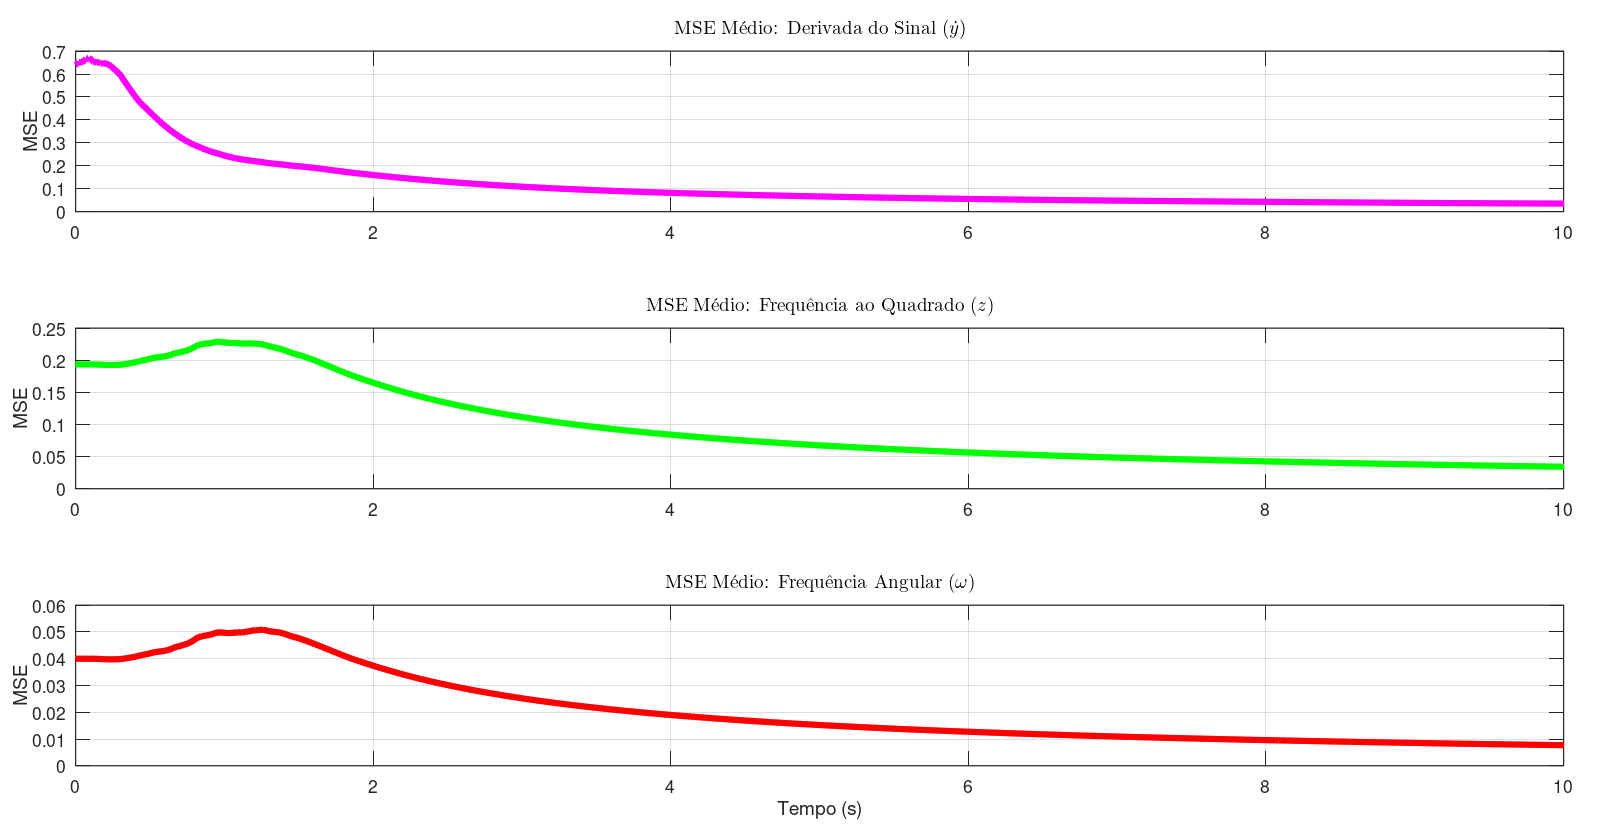
\includegraphics[width=\textwidth]{Figuras/modelo5/M5T1-GER.png}
    \end{minipage}\hfill
    \begin{minipage}{0.48\textwidth}
        \centering
        \caption*{\footnotesize \textbf{(b) MSE da Saídas (Monte Carlo)}}
        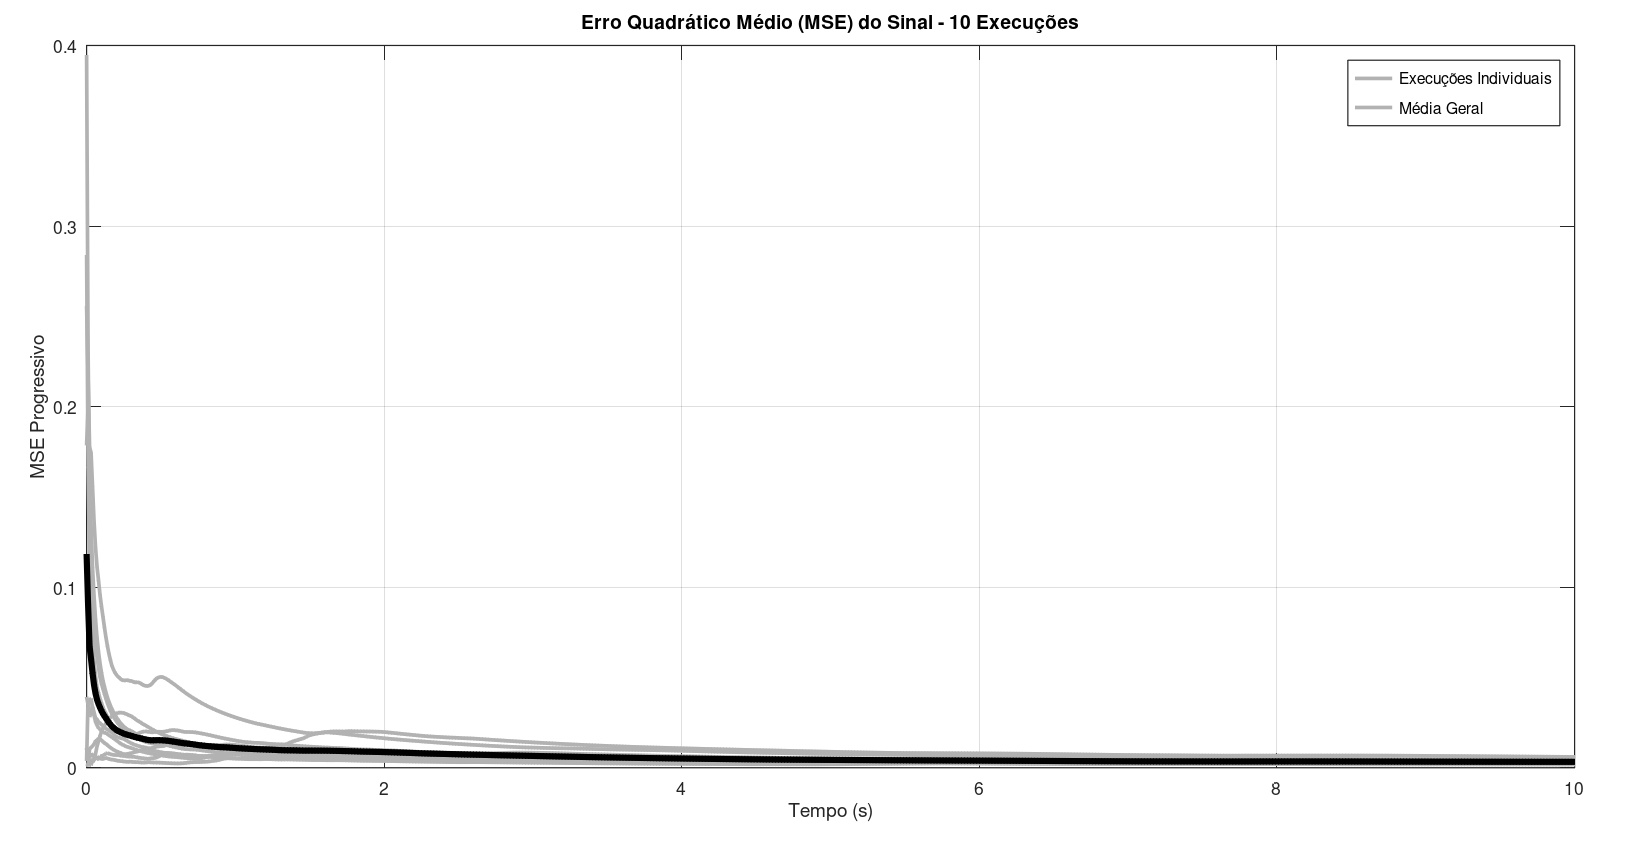
\includegraphics[width=\textwidth]{Figuras/modelo5/M5T1-GERR.png}
    \end{minipage}
    \caption*{\footnotesize \textbf{Fonte:} Elaborado pelo Autor (2026).}
    \label{fig:M5T1CONV_CO}
\end{figure}

\subsubsection{Teste 2: Resolução da Ambiguidade de Sinal}

O Modelo 5 apresenta um comportamento dinâmico análogo ao do Modelo 4, porém com uma vantagem estrutural significativa: a mitigação do problema de ambiguidade de sinal. Ao estimar a frequência ao quadrado ($z = \omega^2$), a formulação contorna a incerteza direcional da inicialização, garantindo a convergência estrita para a frequência angular correta. Esse desempenho superior no rastreamento da dinâmica física pode ser observado na Figura \ref{fig:M5T2G}. 

Adicionalmente, a evolução do Erro Quadrático Médio (MSE), detalhada na Figura \ref{fig:M5T2CONV_CO}, ratifica a estabilidade global do filtro. As curvas evidenciam a minimização consistente tanto das incertezas dos estados internos ($y, \dot{y}, z$) quanto do erro de saída ao longo do regime transiente.

\begin{figure}[H]
    \centering
    \caption{Modelo 5: Estimativas (Teste 2).}
    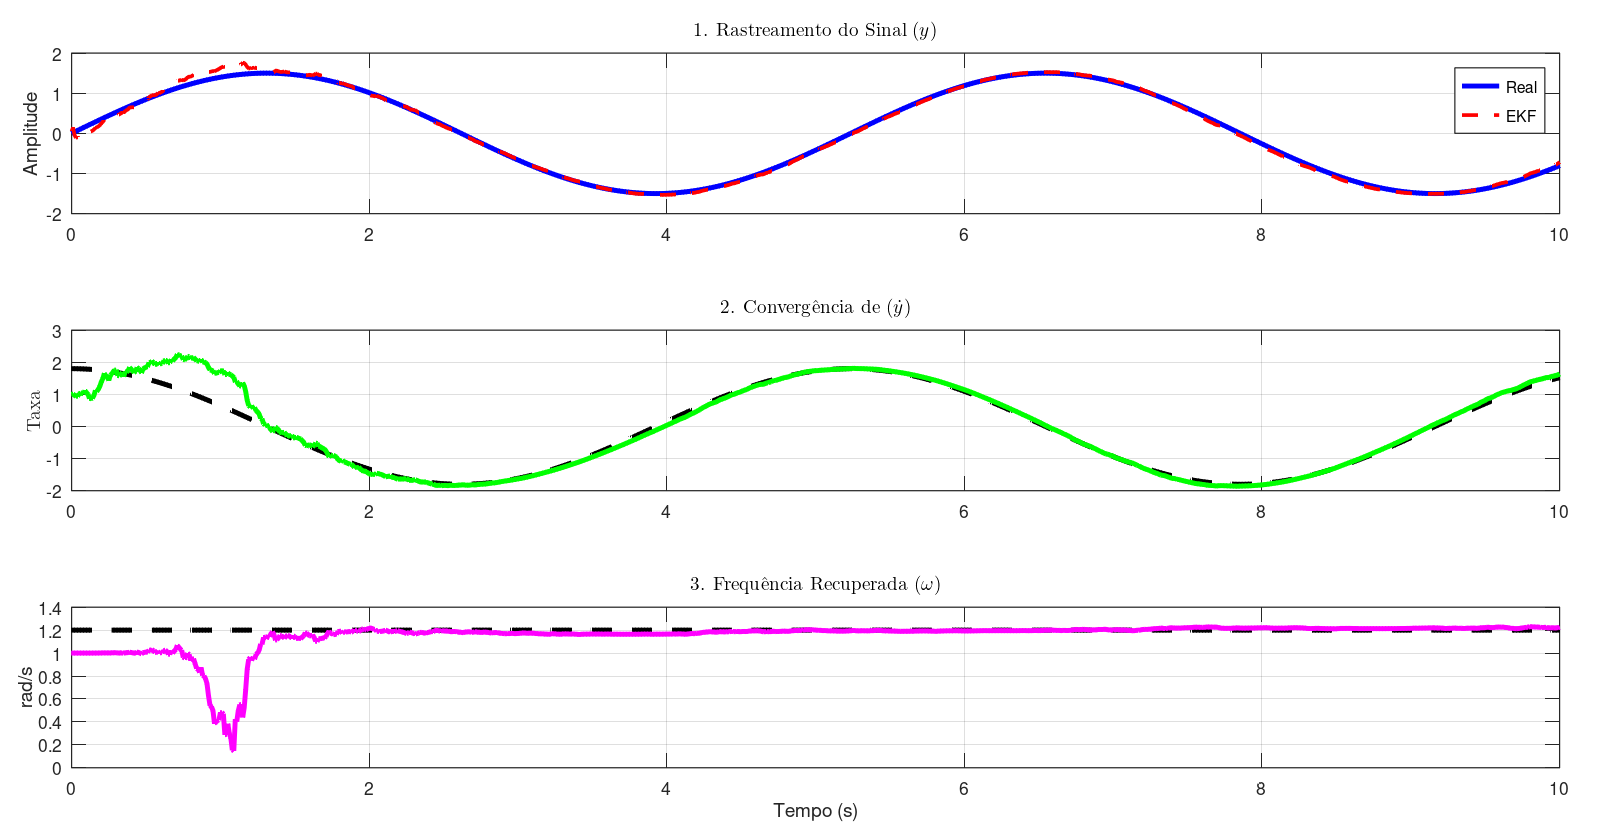
\includegraphics[width=14cm]{Figuras/modelo5/M5T2-GE.png}
    \label{fig:M5T2G}
    \caption*{\footnotesize \textbf{Fonte:} Elaborado pelo Autor (2026).}
\end{figure}

\begin{figure}[H]
    \centering
    \caption{Modelo 5: Convergências do erro (Teste 2).}
    \begin{minipage}{0.48\textwidth}
        \centering
        \caption*{\footnotesize \textbf{(a) MSE dos Estados ($x, \dot{x}, z$)}}
        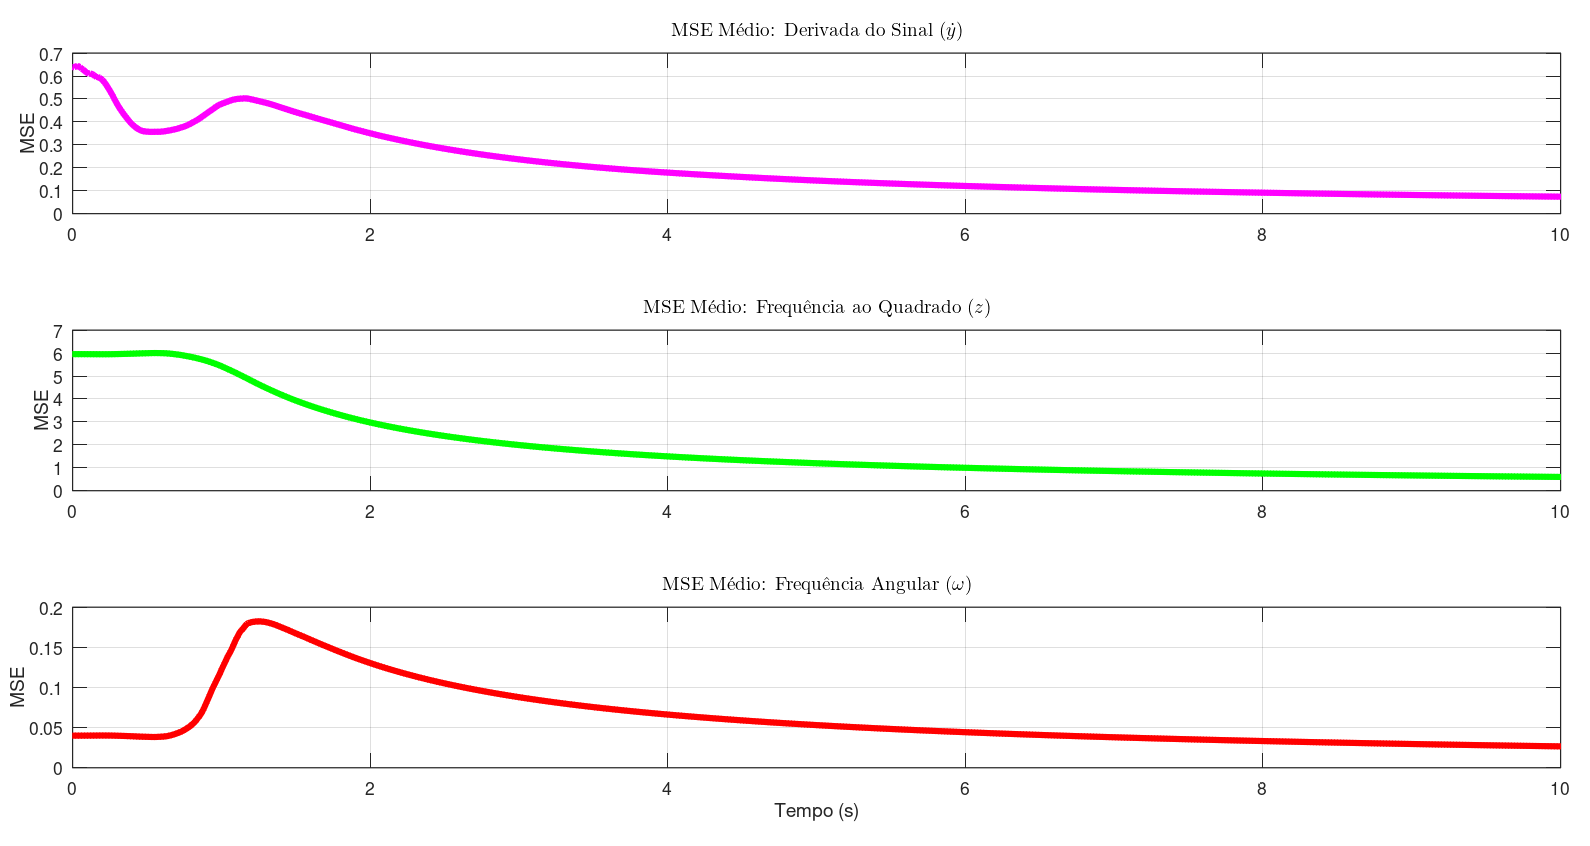
\includegraphics[width=\textwidth]{Figuras/modelo5/M5T2-GER.png}
    \end{minipage}\hfill
    \begin{minipage}{0.48\textwidth}
        \centering
        \caption*{\footnotesize \textbf{(b) MSE da Saídas (Monte Carlo)}}
        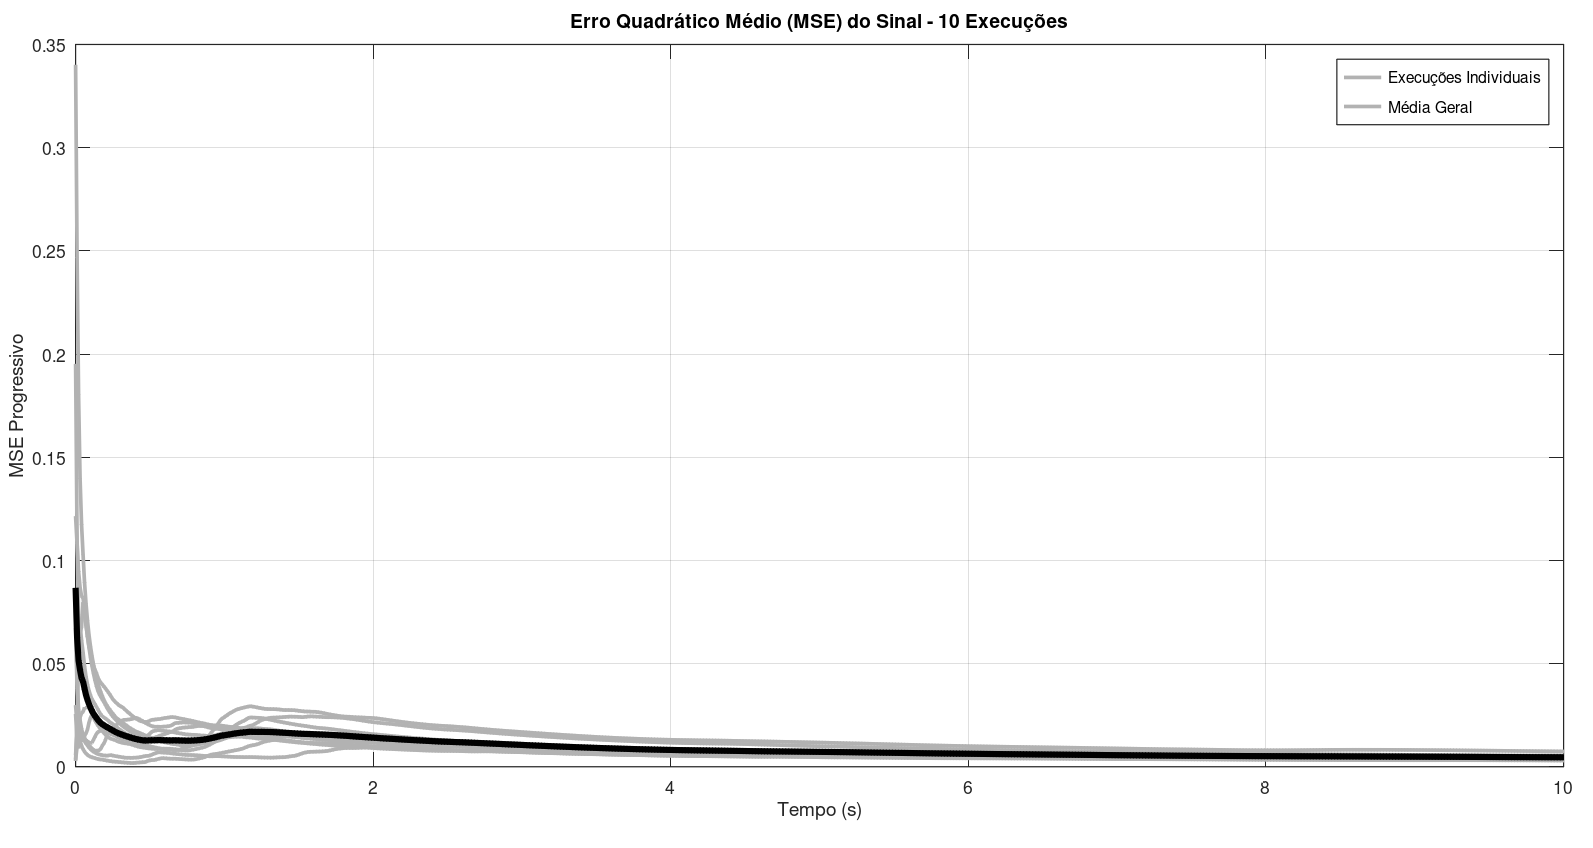
\includegraphics[width=\textwidth]{Figuras/modelo5/M5T2-GERR.png}

    \end{minipage}
    \caption*{\footnotesize \textbf{Fonte:} Elaborado pelo Autor (2026).}
    \label{fig:M5T2CONV_CO}
\end{figure}


\subsubsection{Teste 3: Robustez a estimativa inicial inicial}

O Teste 3 avalia a resiliência do Modelo 5 quando submetido a condições severas de desajuste em sua inicialização. Conforme ilustrado na Figura \ref{fig:M5T3G}, observa-se que o algoritmo demonstra uma notável capacidade de recuperação, convergindo para os parâmetros físicos reais em um intervalo de tempo inferior a um ciclo completo do sinal senoidal ($t < 2\pi/\omega$). Esse comportamento em regime transiente atesta a robustez do estimador diante de entradas adversas.

A análise das curvas de Erro Quadrático Médio, apresentadas na Figura \ref{fig:M5T3CONV_CO}, corrobora esta rápida adaptação. A convergência acelerada tanto das estimativas dos estados internos ($y, \dot{y}, z$) quanto do erro de saída valida a eficácia da matriz de covariância e do ganho de Kalman adaptativo formulados para esta arquitetura.

\begin{figure}[H]
    \centering
    \caption{Modelo 5: Estimativas (Teste 3).}
    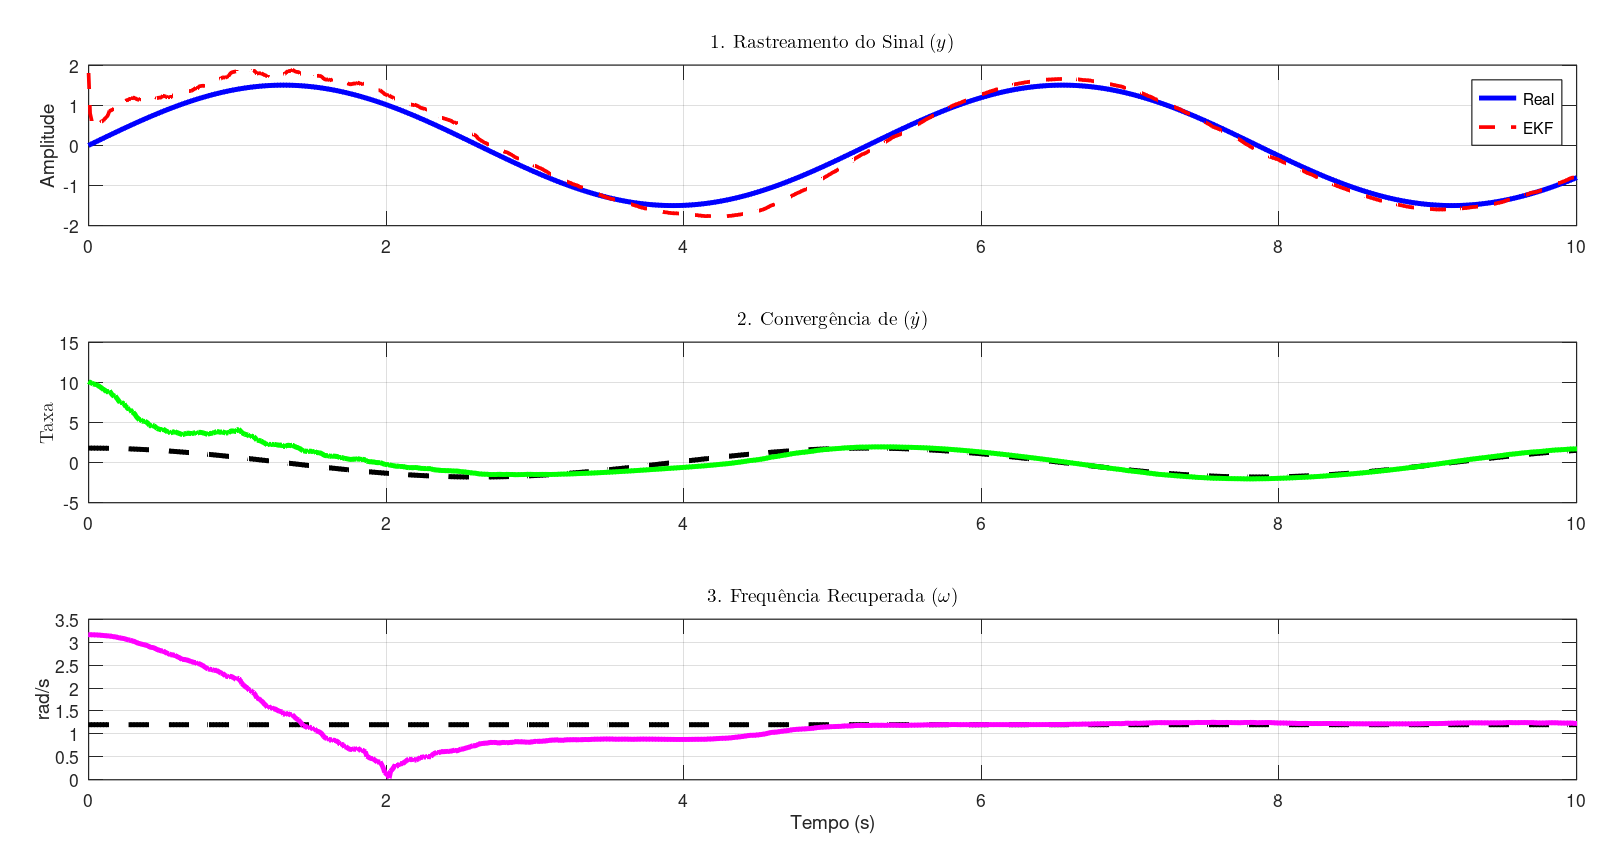
\includegraphics[width=14cm]{Figuras/modelo5/M5T3-GE.png}
    \label{fig:M5T3G}
    \caption*{\footnotesize \textbf{Fonte:} Elaborado pelo Autor (2026).}
\end{figure}

\begin{figure}[H]
    \centering
    \caption{Modelo 5: Convergências do erro (Teste 3).}
    \begin{minipage}{0.48\textwidth}
        \centering
        \caption*{\footnotesize \textbf{(a) MSE dos Estados ($x, \dot{x}, z$)}}
        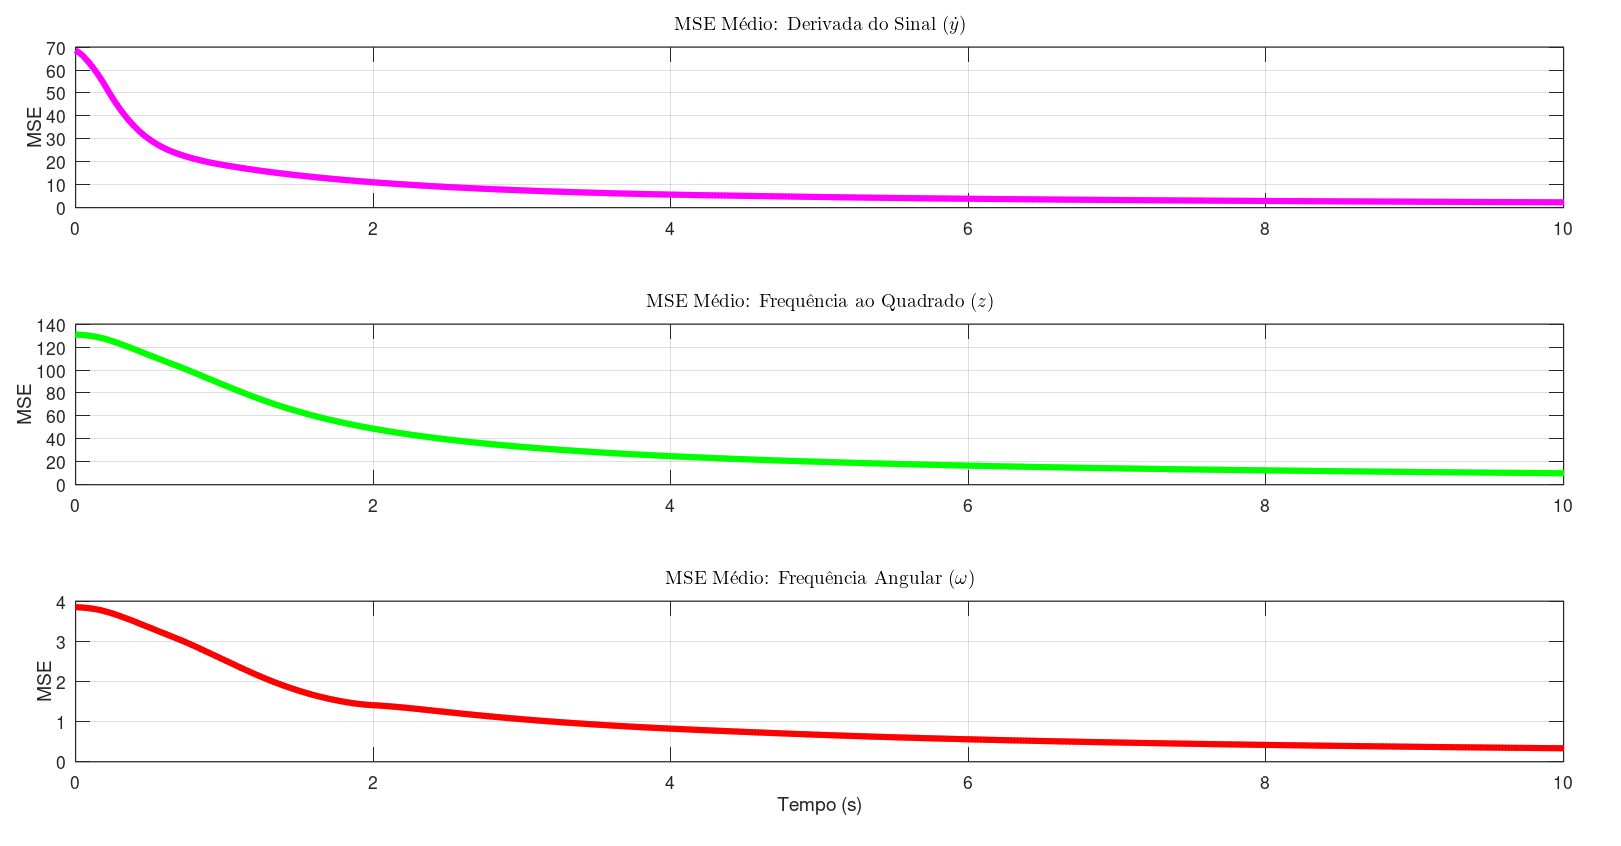
\includegraphics[width=\textwidth]{Figuras/modelo5/M5T3-GER.png}
    \end{minipage}\hfill
    \begin{minipage}{0.48\textwidth}
        \centering
        \caption*{\footnotesize \textbf{(b) MSE da Saídas (Monte Carlo)}}
        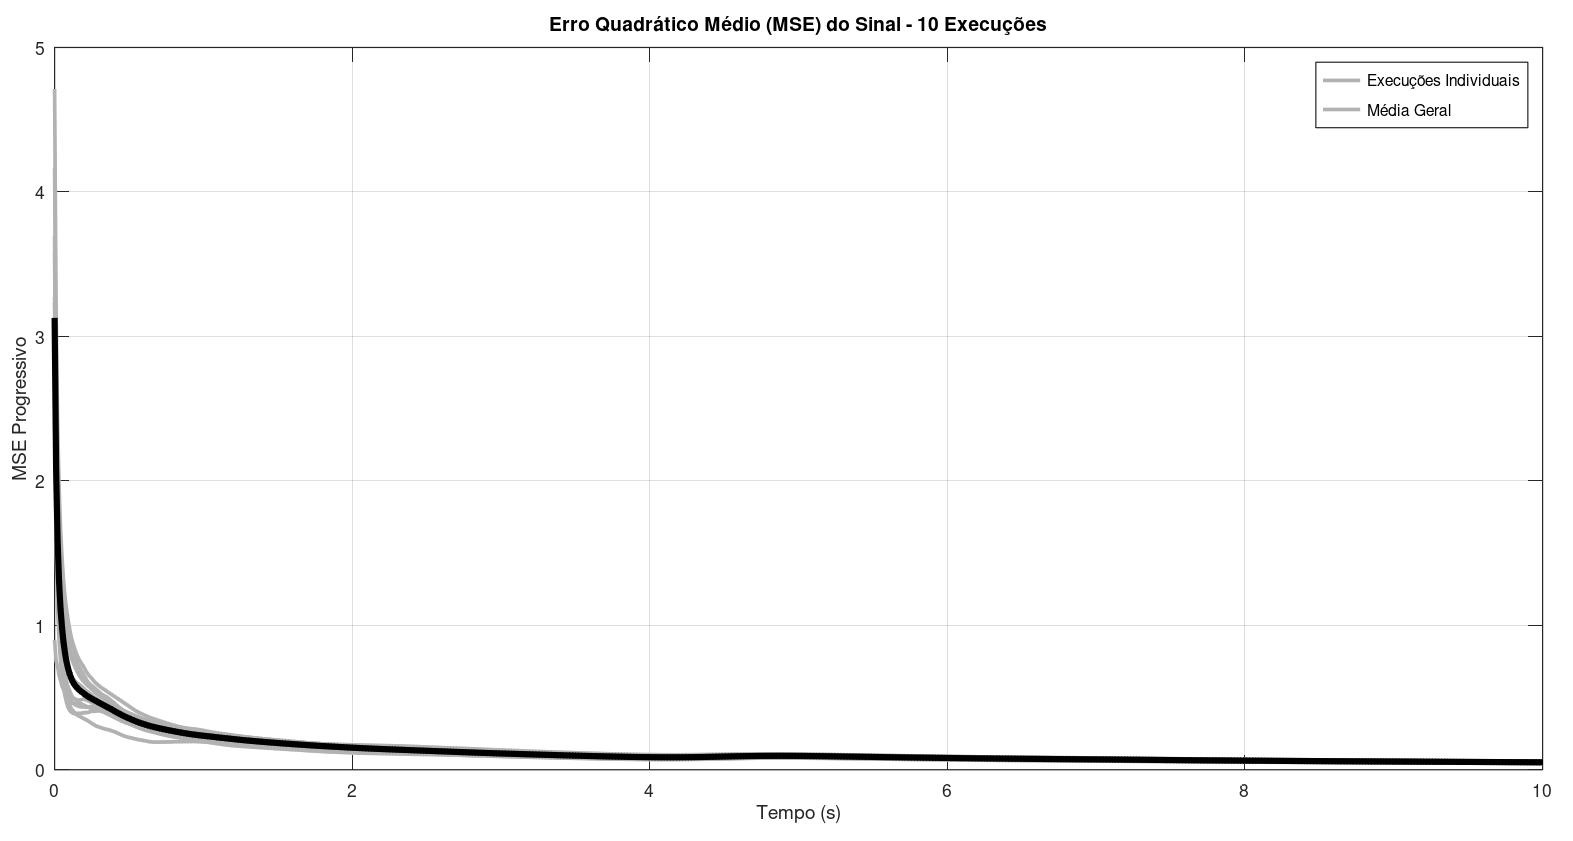
\includegraphics[width=\textwidth]{Figuras/modelo5/M5T3-GERR.png}
    \end{minipage}
    \caption*{\footnotesize \textbf{Fonte:} Elaborado pelo Autor (2026).}
    \label{fig:M5T3CONV_CO}
\end{figure}


\subsubsection{Conclusão Parcial do Modelo 5}
\label{subsubsec:conclusao_m5}

Ao redefinir o terceiro estado do filtro como a frequência angular ao quadrado ($z=\omega^2$), a formulação elimina a ambiguidade de sinal por construção matemática, simplificando significativamente a topologia da função de custo do estimador. Na prática, o desempenho estocástico e os erros de estimação mostraram-se virtualmente idênticos aos obtidos no Modelo 4. Portanto, a introdução da variável $z$ não altera o limite inferior do Erro Quadrático Médio (MSE), mas oferece uma estrutura com observabilidade mais direta e inequivocamente atrelada à física do oscilador. Conclui-se que o Modelo 5 é altamente eficaz na estimação dos estados de sinais senoidais, sobressaindo-se por mitigar o risco de convergência para mínimos locais não físicos \cite{zarchan2015}.

\subsubsection{Síntese Comparativa da Evolução dos Modelos}
\label{subsubsec:sintese_modelos}

A progressão metodológica do Modelo 1 ao Modelo 5 corrobora a premissa de que a definição do espaço de estados é tão determinante para o sucesso da estimação quanto o próprio algoritmo do Filtro de Kalman. Constatou-se que as arquiteturas baseadas em fase explícita (Modelos 2 e 3) são inerentemente suscetíveis a descontinuidades trigonométricas e ambiguidades de sinal. Em contrapartida, as formulações baseadas na dinâmica do oscilador harmônico (Modelos 4 e 5) provaram ser substancialmente mais robustas. Especificamente, a modelagem via frequência ao quadrado (Modelo 5) consolidou-se como a abordagem mais confiável para aplicações práticas com sensores ruidosos, assegurando convergência global e a estrita validade física das estimativas. Em suma, observou-se que a convergência para o estado estacionário ocorreu em um intervalo inferior a um ciclo completo do sinal de referência. Este desempenho no regime transiente é sensível à calibração das matrizes de covariância, podendo ser otimizado mediante o ajuste fino dos parâmetros de processo e medição. Ressalta-se, contudo, que a síntese dos filtros baseou-se no conhecimento prévio da estatística dos ruídos. Em aplicações reais, onde as propriedades estocásticas são incertas, a etapa de sintonização (tuning) exige uma caracterização experimental rigorosa das variâncias para assegurar a otimalidade do estimador.

\subsection{Análise Comparativa Global}
\label{subsec:analise_comparativa}

A Tabela \ref{tab:comparativo} sintetiza as métricas de desempenho das arquiteturas avaliadas ao longo deste estudo. O Modelo 5 consolida-se como a solução de maior destaque, promovendo um balanço ótimo entre a precisão do rastreamento em regime permanente e a imunidade total a erros grosseiros de inicialização.

\begin{table}[H]
    \centering
    \caption{Comparativo global de Robustez e Precisão dos Modelos da Senoide}
    \vspace{0.2cm}
    \begin{tabular}{|p{4.0cm}|c|c|c|}
        \hline
        \textbf{Modelo} & \textbf{MSE Sinal} & \textbf{Robustez Inicial} & \textbf{Observabilidade} \\ \hline
        1 LKF ($\left[y; \dot{y}\right]$)         & Mínimo*     & Alta            & Total                    \\ \hline
        2 EKF ($\left[\phi; \omega; A \right]$)   & Alto        & Baixa          & Parcial                  \\ \hline
        3  EKF ($\left[\phi; \omega\right]$)           & Médio       & Moderada       & Total                  \\ \hline
        4 EKF ($\left[y; \dot{y}; \omega \right]$)     &  Baixo      & Boa            & Parcial      \\ \hline
        5 EKF ($\left[y; \dot{y}; \omega^2\right]$) & Muito Baixo & Elevada        & Total                    \\ \hline
    \end{tabular}
    \label{tab:comparativo}
    \caption*{\footnotesize \textbf{Fonte:} Elaborado pelo autor (2026). \newline * \textit{Refere-se ao limite teórico ótimo por tratar-se de um modelo linear com parâmetros conhecidos.}}
\end{table}

    % --- Tabela com estimativas de MSE (visualmente estimadas a partir dos gráficos de Monte Carlo) ---
    \begin{table}[H]
    \centering
    \caption{Estimativa do MSE (inicial e convergido) e tempo até quasi-estacionário (Monte Carlo, 10 execuções).}
    \label{tab:mse_montecarlo_estimada}
    \begin{tabular}{l|c|c|c}
    \hline
    \textbf{Modelo / Teste} & \textbf{MSE inicial} & \textbf{MSE Final} & \textbf{Tempo. Estacionário (s)} \\\hline
    1 LKF - Teste 1 & 0,06 & 0,001 & 0,3 \\
    1 LKF - Teste 2 & 0,06 & 0,001 & 0,3 \\
    1 LKF - Teste 3 & 0,25 & 0,005 & 0,5 \\
    1 LKF - Teste 4 & 0,08 & 0,002 & 0,4 \\
    \hline
    2 EKF - Teste 1 & 0,06 & 0,002 & 0,5 \\
    2 EKF - Teste 2 & 0,20 & 0,010 & 1,0 \\
    2 EKF - Teste 3 & 0,40 & 0,020 & 1,5 \\
    \hline
    3 EKF - Teste 1 & 0,05 & 0,001 & 0,4 \\
    3 EKF - Teste 2 & 0,06 & 0,001 & 0,4 \\
    3 EKF - Teste 3 & 0,08 & 0,002 & 0,5 \\
    \hline
    4 EKF - Teste 1 & 0,20 & 0,010 & 0,6 \\
    4 EKF - Teste 2 & 0,25 & 0,015 & 0,7 \\
    4 EKF - Teste 3 & 0,60 & 0,030 & 1,2 \\
    \hline
    5 EKF - Teste 1 & 0,15 & 0,005 & 0,5 \\
    5 EKF - Teste 2 & 0,18 & 0,006 & 0,6 \\
    5 EKF - Teste 3 & 0,50 & 0,020 & 1,0 \\
    \hline
    \end{tabular}
    \caption*{\footnotesize \textbf{Fonte:} Elaborado pelo autor (2026).}
    \end{table}

    A Tabela \ref{tab:mse_montecarlo_estimada} resume as estimativas visuais do erro quadrático médio (MSE) no instante inicial e em regime convergido, bem como o tempo aproximado até o comportamento quasi-estacionário para cada modelo e teste. Observa-se, a partir dos valores apresentados, que:

    \begin{itemize}
        \item Os Modelos 1 e 3 alcançam os menores valores de MSE convergido (ordem de $10^{-3}$ a $10^{-2}$) e apresentam tempos de evolução mais rápidos (aprox. 0,3–0,4 s), indicando convergência rápida quando as hipóteses lineares ou moderadas se mantêm.
        \item O Modelo 4 exibe tanto MSE inicial mais elevado quanto MSE convergido maior, além de tempos de estabilização superiores (até ~1,2 s), o que sugere sensibilidade às não linearidades e pior ajuste em regime estacionário.
        \item O Modelo 2 apresenta comportamento intermediário: em alguns testes (ex.: Teste 3) a convergência é lenta e o MSE convergido maior, apontando para menor robustez frente a variações paramétricas.
        \item O Modelo 5 combina MSE convergido competitivo com tempos de convergência moderados, o que corrobora sua utilidade prática apontada anteriormente; sua performance sugere um bom compromisso entre precisão de estado e robustez numérica.
    \end{itemize}

    Essas conclusões, extraídas da Tabela \ref{tab:mse_montecarlo_estimada}, devem ser interpretadas com cautela: como indicado na legenda, os números são estimativas visuais a partir das figuras de Monte Carlo e destinam-se a dar uma intuição sobre a velocidade de evolução de cada método. Para comparações quantitativas rigorosas, recomenda-se substituir estes valores por métricas computadas diretamente a partir dos vetores de erro gerados nos scripts (saída do GNU Octave) e, preferencialmente, apresentar intervalos de confiança sobre a média Monte Carlo.

    Em suma, enquanto o Modelo 1 estabelece o referencial teórico ótimo para o problema, o Modelo 5 demonstrou ser a implementação prática mais resiliente. Esta arquitetura supera com êxito as limitações intrínsecas do Filtro de Kalman Estendido (EKF) ao lidar com não linearidades severas de natureza trigonométrica, garantindo estabilidade analítica e viabilizando sua aplicação confiável em sistemas de tempo real.

\newpage
\section{CONCLUSÃO}
\label{sec:conclusao}

Este estudo demonstrou que a eficácia do Filtro de Kalman Estendido (EKF) no rastreio de sinais senoidais não é garantida por uma escolha arbitrária de modelagem, mas reside na convergência entre a arquitetura do espaço de estados e os requisitos específicos da aplicação. Evidenciou-se que a seleção do modelo não é um processo trivial; modelos parametrizados diretamente em fase, frequência e amplitude (Modelos 2 e 3) revelaram vulnerabilidades críticas de observabilidade, tornando-se susceptíveis a mínimos locais sob inicializações imprecisas. Portanto, cabe ao projetista realizar uma análise criteriosa da topologia do sistema, compreendendo que a robustez estrutural precede os ajustes paramétricos.

Neste contexto, a transição para modelos baseados na dinâmica do oscilador harmônico representou um avanço significativo. O \textbf{Modelo 5} consolidou-se como a abordagem superior ao definir o estado como a frequência angular ao quadrado ($z = \omega^2$). Esta estratégia permite a linearização parcial das relações de estado e elimina, por construção matemática, a ambiguidade de sinal, garantindo um rastreio estável e fisicamente coerente mesmo sob condições iniciais adversas ou ruidosas.

Paralelamente à estrutura do modelo, observou-se que a funcionalidade plena do algoritmo é estritamente condicionada à definição precisa das matrizes de covariância do ruído de processo ($Q$) e de medição ($R$). Embora nesta pesquisa a suposição de valores ótimos tenha sido facilitada pela natureza controlada dos testes, em cenários práticos de instrumentação, essa definição assume um caráter empírico e complexo. Este processo, tecnicamente denominado \textit{sintonização} (ou \textit{tuning}) do Filtro de Kalman, constitui um dos maiores desafios da engenharia de controle, exigindo do projetista uma compreensão profunda do balanço entre a rapidez de resposta e a imunidade ao ruído.

Em suma, o trabalho conclui que o sucesso na extração de informações de sensores ruidosos depende de um compromisso entre uma estrutura de estados que minimize singularidades e uma sintonização rigorosa das estatísticas de ruído. O Modelo 5 provou ser a ferramenta mais resiliente para superar as não linearidades intrínsecas ao rastreio senoidal, estabelecendo-se como uma base confiável para o desenvolvimento de sensores inteligentes e sistemas de processamento de sinais em tempo real.

\newpage 
\bibliography{referencias} % Puxa o arquivo referencias.bib

\newpage

\appendix
\section{Solução da equação de estados homogênea}
\label{anm:solucao_edo}

Considere a forma homogênea da equação de estados no domínio do tempo contínuo:
\begin{equation}
    \dot{\mathbf{x}}(t) = \mathbf{A}\mathbf{x}(t)
    \label{eq:homoEQ}
\end{equation}

Para o caso escalar, definido por $\dot{x}(t) = ax(t)$, a solução geral para $t > t_0$ é dada por:
\begin{equation}
    x(t) = e^{a(t-t_0)}x(t_0)
\end{equation}

Dessa forma, espera-se que a solução para a forma vetorial apresente uma estrutura semelhante. O ponto de partida consiste em expandir o termo exponencial $e^x$ em sua série de potências de Taylor:
\begin{equation}
    e^x = \exp(x) = \left( 1 + x + \frac{x^2}{2!} + \dots + \frac{x^k}{k!} + \dots \right) = \sum_{n=0}^{\infty} \frac{x^n}{n!}, \quad \forall x \in \mathbb{R}
    \label{eq:taylor1}
\end{equation}

Aplicando esta expansão ao caso escalar da solução do sistema, temos:
\begin{equation}
    x(t) = \left( \sum_{n=0}^{\infty} \frac{a^n(t-t_0)^n}{n!} \right) x(t_0)
\end{equation}

Considerando o caso em que $t_0=0$, temos

\begin{equation}
    x(t) = \left( \sum_{n=0}^{\infty} \frac{(at)^n }{n!} \right) x(0)
    \label{eq:taylor}
\end{equation}

Assume-se, por hipótese, que a solução para o caso vetorial descrito na Equação \eqref{eq:homoEQ} também possa ser expressa como uma série de potências de matrizes:
\begin{equation}
    \mathbf{x}(t) = \mathbf{b}_0 + \mathbf{b}_1 t + \mathbf{b}_2 t^2 + \dots + \mathbf{b}_k t^k + \dots
    \label{eq:homoEQ2}
\end{equation}

Substituindo a Equação \eqref{eq:homoEQ2} em \eqref{eq:homoEQ}, obtém-se:
\begin{equation}
    \frac{d}{dt} \left( \sum_{k=0}^{\infty} \mathbf{b}_k t^k \right) = \mathbf{A} \left( \sum_{k=0}^{\infty} \mathbf{b}_k t^k \right)
\end{equation}

Calculando a derivada temporal do lado esquerdo e expandindo os termos:
\begin{equation}
    \mathbf{b}_1 + 2\mathbf{b}_2 t + 3\mathbf{b}_3 t^2 + \dots + k\mathbf{b}_k t^{k-1} + \dots = \mathbf{A}\mathbf{b}_0 + \mathbf{A}\mathbf{b}_1 t + \mathbf{A}\mathbf{b}_2 t^2 + \dots
\end{equation}

Ao igualar os coeficientes das potências de $t$ correspondentes, resulta no seguinte sistema de equações lineares:
\begin{equation}
    \begin{cases}
        \mathbf{b}_1 = \mathbf{A}\mathbf{b}_0 \\
        2\mathbf{b}_2 = \mathbf{A}\mathbf{b}_1 \\
        3\mathbf{b}_3 = \mathbf{A}\mathbf{b}_2 \\
        \vdots \\
        k\mathbf{b}_k = \mathbf{A}\mathbf{b}_{k-1}
    \end{cases}
\end{equation}

Este sistema define uma relação recursiva para os coeficientes $\mathbf{b}_k$, dada por:
\begin{equation}
    \mathbf{b}_k = \frac{\mathbf{A}\mathbf{b}_{k-1}}{k} 
    \label{eq:recEq}
\end{equation}

Ao desenvolver a recursão, observa-se o surgimento do fatorial no denominador:
\begin{equation}
    \mathbf{b}_k = \frac{\mathbf{A}}{k} \left( \frac{\mathbf{A}\mathbf{b}_{k-2}}{k-1} \right) = \frac{\mathbf{A}^2}{k(k-1)} \mathbf{b}_{k-2} = \dots = \frac{\mathbf{A}^k}{k!} \mathbf{b}_0
\end{equation}

Substituindo os coeficientes $\mathbf{b}_k$ na série original e isolando o vetor constante $\mathbf{b}_0$:
\begin{equation}
    \mathbf{x}(t) = \left( \mathbf{I} + \mathbf{A}t + \frac{\mathbf{A}^2 t^2}{2!} + \dots + \frac{\mathbf{A}^k t^k}{k!} + \dots \right) \mathbf{b}_0
\end{equation}

Empregando a notação de somatório, a expressão torna-se:
\begin{equation}
    \mathbf{x}(t) = \left( \sum_{n=0}^{\infty} \frac{\mathbf{A}^n t^n}{n!} \right) \mathbf{b}_0
\end{equation}

Ao avaliar a solução para o instante inicial $t=0$, verifica-se que $\mathbf{x}(0) = \mathbf{b}_0$. Portanto, a solução da equação homogênea é:
\begin{equation}
    \mathbf{x}(t) = \left( \sum_{n=0}^{\infty} \frac{(\mathbf{A}t)^n}{n!} \right) \mathbf{x}(0)
\end{equation}

Esta série de potências matriciais é definida como a matriz exponencial, denotada por $\exp(\mathbf{A}t)$ ou $e^{\mathbf{A}t}$. Assim, a solução final assume a forma compacta:
\begin{equation}
    \mathbf{x}(t) = e^{\mathbf{A}t} \mathbf{x}(0)
\end{equation}

Este resultado é formalmente equivalente à solução encontrada para o caso escalar, estendendo o conceito de exponencial para operadores matriciais.
% ==============================
\newpage
\section{Solução geral de estados não-homogênea com ruído de processo}
\label{anm:solucao_edo_erro}

O caso mais abrangente na modelagem ocorre quando consideramos as incertezas do sistema, representadas pelo vetor de ruído de processo $\mathbf{w}(t)$. A equação de transição de estados assume, então, a seguinte forma:
\begin{equation}
    \dot{\mathbf{x}}(t) = \mathbf{A}\mathbf{x}(t) + \mathbf{B}\mathbf{u}(t) + \mathbf{w}(t)
    \label{eq:eqComRuido}
\end{equation}

Uma estratégia eficiente para resolver esta equação diferencial consiste em agrupar os termos que envolvem o vetor de estados $\mathbf{x}(t)$ e utilizar o fator integrante matricial $e^{-\mathbf{A}t}$:
\begin{equation}
    \dot{\mathbf{x}}(t) - \mathbf{A}\mathbf{x}(t) = \mathbf{B}\mathbf{u}(t) + \mathbf{w}(t)
\end{equation}

Multiplicando ambos os lados da igualdade à esquerda pelo fator integrante:
\begin{equation}
    e^{-\mathbf{A}t} \left[ \dot{\mathbf{x}}(t) - \mathbf{A}\mathbf{x}(t) \right] = e^{-\mathbf{A}t} \mathbf{B}\mathbf{u}(t) + e^{-\mathbf{A}t} \mathbf{w}(t)
\end{equation}

Observa-se que o lado esquerdo da igualdade corresponde exatamente à derivada temporal do produto entre a matriz exponencial e o vetor de estados, visto que $\frac{d}{dt}\left(e^{-\mathbf{A}t}\right) = -\mathbf{A}e^{-\mathbf{A}t}$. Assim, a equação simplifica-se para:
\begin{equation}
    \frac{d}{dt} \left( e^{-\mathbf{A}t} \mathbf{x}(t) \right) = e^{-\mathbf{A}t} \mathbf{B}\mathbf{u}(t) + e^{-\mathbf{A}t} \mathbf{w}(t)
\end{equation}

Integrando ambos os lados em relação a uma variável auxiliar $\tau$, no intervalo de $t_0$ a $t$:
\begin{equation}
    \int_{t_0}^t \frac{d}{d\tau} \left( e^{-\mathbf{A}\tau} \mathbf{x}(\tau) \right) d\tau = \int_{t_0}^t \left( e^{-\mathbf{A}\tau} \mathbf{B}\mathbf{u}(\tau) + e^{-\mathbf{A}\tau} \mathbf{w}(\tau) \right) d\tau
\end{equation}

Pelo Teorema Fundamental do Cálculo, o lado esquerdo resulta na diferença da função avaliada nos limites de integração:
\begin{equation}
    e^{-\mathbf{A}t}\mathbf{x}(t) - e^{-\mathbf{A}t_0}\mathbf{x}(t_0) = \int_{t_0}^t e^{-\mathbf{A}\tau} \mathbf{B}\mathbf{u}(\tau) d\tau + \int_{t_0}^t e^{-\mathbf{A}\tau} \mathbf{w}(\tau) d\tau
\end{equation}

Isolando o termo que contém $\mathbf{x}(t)$ e multiplicando toda a equação à esquerda por $e^{\mathbf{A}t}$, obtemos:
\begin{equation}
    \mathbf{x}(t) = e^{\mathbf{A}t} e^{-\mathbf{A}t_0} \mathbf{x}(t_0) + e^{\mathbf{A}t} \int_{t_0}^t e^{-\mathbf{A}\tau} \mathbf{B}\mathbf{u}(\tau) d\tau + e^{\mathbf{A}t} \int_{t_0}^t e^{-\mathbf{A}\tau} \mathbf{w}(\tau) d\tau
\end{equation}

Dado que a matriz exponencial $e^{\mathbf{A}t}$ é independente da variável de integração $\tau$, ela pode ser deslocada para o interior dos integrandos. Combinando as exponenciais através da propriedade $e^{\mathbf{M}}e^{\mathbf{N}} = e^{\mathbf{M+N}}$ (válida pois $\mathbf{A}t$ e $-\mathbf{A}\tau$ comutam), chega-se à solução geral:
\begin{equation}
    \mathbf{x}(t) = e^{\mathbf{A}(t-t_0)}\mathbf{x}(t_0) + \int_{t_0}^t e^{\mathbf{A}(t-\tau)} \mathbf{B}\mathbf{u}(\tau) d\tau + \int_{t_0}^t e^{\mathbf{A}(t-\tau)} \mathbf{w}(\tau) d\tau
    \label{eq:SolucaoGeral3}
\end{equation}


A Equação \eqref{eq:SolucaoGeral3} demonstra que a evolução do estado do sistema é composta pela superposição de três parcelas: a resposta à entrada nula (dependente apenas da condição inicial), a resposta determinística ao estado nulo (resultante da convolução com o sinal de controle) e a resposta estocástica (resultante da acumulação do ruído de processo no intervalo considerado). Observe também que caso $\mathbf{w}(t) = \mathbf{0}$, a Equação \ref{eq:SolucaoGeral3} decai na Equação \ref{eq:SoluçãoGeral2}, que seria o caso ideal, sem erros no processo do modelo.

\begin{equation}
    \mathbf{x}(t) = e^{\mathbf{A}(t-t_0)}\mathbf{x}(t_0) + \int_{t_0}^t e^{\mathbf{A}(t-\tau)} \mathbf{B}\mathbf{u}(\tau) d\tau
    \label{eq:SoluçãoGeral2}
\end{equation}

\section{Linearização da dinâmica do erro de estimação para o Filtro de Kalman Estendido}
\label{anm:solucao_edo_geral}

A fundamentação para a linearização de sistemas dinâmicos não lineares no contexto da filtragem estendida baseia-se na expansão em Série de Taylor de primeira ordem. Para uma função vetorial de múltiplas variáveis $\mathbf{h}(\mathbf{z})$, a expansão em torno de um ponto de operação nominal $\mathbf{z}_0$ é definida por:

\begin{equation}
    \mathbf{h}(\mathbf{z}) \approx \mathbf{h}(\mathbf{z}_0) + \left. \frac{\partial \mathbf{h}}{\partial \mathbf{z}} \right|_{\mathbf{z}=\mathbf{z}_0} (\mathbf{z} - \mathbf{z}_0)
    \label{eq:taylor_multivariavel}
\end{equation}

Considere o modelo de estados do sistema definido na Equação \eqref{eq:EqEstados_estocastico}. No Filtro de Kalman Estendido (EKF), não linearizamos o sistema em torno de um ponto de equilíbrio estático, mas sim em torno da própria trajetória nominal estimada, dada por $(\hat{\mathbf{x}}(t), \mathbf{u}(t))$. 

Para tal, definem-se as variáveis de desvio (ou perturbação) como a diferença entre o estado verdadeiro e o estado nominal:
\begin{equation}
    \Delta\mathbf{x}(t) = \mathbf{x}(t) - \hat{\mathbf{x}}(t)
\end{equation}

Aplicando a expansão de Taylor \eqref{eq:taylor_multivariavel} na equação diferencial não linear do sistema e desprezando os termos de ordem superior, obtemos:
\begin{equation}
    \dot{\mathbf{x}}(t) \approx \mathbf{f}(\hat{\mathbf{x}}(t), \mathbf{u}(t), t) + \mathbf{F}(t)\Delta\mathbf{x}(t) + \mathbf{w}(t)
\end{equation}

Sabendo que a dinâmica da trajetória nominal é regida puramente pela parte determinística do modelo não linear, ou seja, $\dot{\hat{\mathbf{x}}}(t) = \mathbf{f}(\hat{\mathbf{x}}(t), \mathbf{u}(t), t)$, e que $\dot{\mathbf{x}}(t) = \dot{\hat{\mathbf{x}}}(t) + \Delta\dot{\mathbf{x}}(t)$, os termos não lineares se cancelam. A dinâmica assume, portanto, a sua forma linearizada estritamente em função das variáveis de desvio:
\begin{equation}
    \begin{cases}
        \Delta\dot{\mathbf{x}}(t) \approx \mathbf{F}(t)\Delta\mathbf{x}(t) + \mathbf{w}(t) \\
        \Delta\mathbf{y}(t) \approx \mathbf{H}(t)\Delta\mathbf{x}(t) + \mathbf{v}(t)
    \end{cases}
    \label{eq:dinamica_linearizada_total}
\end{equation}

Nesta formulação, as matrizes do sistema são obtidas através do cálculo dos Jacobianos das funções $\mathbf{f}$ e $\mathbf{g}$, avaliados continuamente na estimativa atual $\hat{\mathbf{x}}(t)$. A matriz de dinâmica $\mathbf{F}(t)$ e a matriz de observação $\mathbf{H}(t)$ são definidas como:
\begin{equation}
    \mathbf{F}(t) = \left. \frac{\partial \mathbf{f}}{\partial \mathbf{x}} \right|_{\hat{\mathbf{x}}, \mathbf{u}} = 
    \begin{bmatrix}
        \frac{\partial f_1}{\partial x_1} & \cdots & \frac{\partial f_1}{\partial x_n} \\
        \vdots & \ddots & \vdots \\
        \frac{\partial f_n}{\partial x_1} & \cdots & \frac{\partial f_n}{\partial x_n}
    \end{bmatrix}, \quad
    \mathbf{H}(t) = \left. \frac{\partial \mathbf{g}}{\partial \mathbf{x}} \right|_{\hat{\mathbf{x}}, \mathbf{u}} = 
    \begin{bmatrix}
        \frac{\partial g_1}{\partial x_1} & \cdots & \frac{\partial g_1}{\partial x_n} \\
        \vdots & \ddots & \vdots \\
        \frac{\partial g_p}{\partial x_1} & \cdots & \frac{\partial g_p}{\partial x_n}
    \end{bmatrix}
\end{equation}

A representação em espaço de estados linearizada para as variáveis de desvio permite a aplicação direta da solução por fator integrante, conforme desenvolvido no Anexo \ref{anm:solucao_edo_erro}. Rigorosamente, por se tratar de um sistema Variante no Tempo (LTV), a solução exigiria a integral de Magnus. Contudo, assumindo-se a premissa de que o Jacobiano $\mathbf{F}(t)$ permanece aproximadamente constante durante um intervalo de amostragem suficientemente pequeno (invariância local), a evolução do erro de estimação entre $t_0$ e $t$ é dada por:

\begin{equation}
    \Delta\mathbf{x}(t) = e^{\mathbf{F}(t)(t-t_0)}\Delta\mathbf{x}(t_0) + \int_{t_0}^t e^{\mathbf{F}(t)(t-\tau)} \mathbf{w}(\tau) d\tau
    \label{eq:SolucaoGeralLinearizada_Erro}
\end{equation}

Esta separação conceitual é o cerne do Filtro de Kalman Estendido: enquanto a estimativa do estado $\hat{\mathbf{x}}(t)$ evolui através do modelo não linear original, garantindo a integridade física do sistema, as matrizes de covariância (que representam a incerteza estatística de $\Delta\mathbf{x}$) são propagadas utilizando a solução linearizada \eqref{eq:SolucaoGeralLinearizada_Erro}.

\end{document}